\documentclass[aspectratio=169, usenames, dvipsnames]{beamer}

%%%%%
%%%%%
%%%%%     DEFINE THE THEME USED
%%%%%
%%%%%

\usetheme{jc}

%%%%%%%%%%%%%%%%%%%%%%%%%%%%%%%%%%%%%%%%%%%%%%%%%
%%%%%                                       %%%%%
%%%%%     LIST OF USEFUL LaTeX PACKAGES     %%%%%
%%%%%                                       %%%%%
%%%%%%%%%%%%%%%%%%%%%%%%%%%%%%%%%%%%%%%%%%%%%%%%%

% ---
% Character encoding
% ---
\usepackage[T1]{fontenc}
\usepackage[utf8]{inputenc}

% ---
% Language related packages
% ---
\usepackage[english]{babel}
\usepackage[abbreviations,british]{foreign}

% ---
% Bibliography-related
% ---
\usepackage[numbers, sort&compress]{natbib}

% ---
% Colours
% ---
\usepackage[]{color}
\usepackage[]{xcolor}

% ---
% Figures
% ---
\usepackage[]{graphicx}
\usepackage[]{subfigure}

\graphicspath{{imgs/}}

% ---
% Mathematics
% ---
\usepackage[]{mathtools}
\usepackage[]{amssymb, amsmath, amsfonts}
\usepackage[]{yhmath}
\usepackage[]{stmaryrd}
\usepackage[]{nicefrac}

% ---
% Physics
% ---
\usepackage[]{siunitx}
\usepackage[]{physics}

% ---
% Tikz-related
% ---
\usepackage[]{tikz}
\usetikzlibrary{arrows}
\usetikzlibrary{shapes}
\usetikzlibrary{positioning}
\usetikzlibrary{tikzmark}
\usetikzlibrary{patterns}
\usetikzlibrary{backgrounds}

% ---
% PGF related
% ---
\usepackage{pgfplots}
\pgfplotsset{compat=newest}

% ---
% Miscellaneous
% ---
\usepackage[]{lipsum}
\usepackage[]{xparse}
\usepackage[]{multicol}

%%%%%%%%%%%%%%%%%%%%%%%%%%%%%%%%%%%%%%%%%%%%%%%
%%%%%                                     %%%%%
%%%%%     LIST OF COMMANDS AND MACROS     %%%%%
%%%%%                                     %%%%%
%%%%%%%%%%%%%%%%%%%%%%%%%%%%%%%%%%%%%%%%%%%%%%%

\newcommand{\redline}{\raisebox{2pt}{\tikz{\draw[-, thick, red, dashed, line width = 0.9pt](0,0) -- (5mm,0);}}}
\newcommand{\blueline}{\raisebox{2pt}{\tikz{\draw[-, thick, blue!67, solid, line width = 0.9pt](0,0) -- (5mm,0);}}}

% ---
% Annotating equations using Tikz
% ---
\newcommand{\highlight}[2]{\colorbox{#1!17}{\ensuremath{\displaystyle #2}}}
\newcommand{\highlightdark}[2]{\colorbox{#1!47}{\ensuremath{\displaystyle #2}}}

% ---
% Mathematics
% ---

% Simple macros
\renewcommand{\det}[1]{\text{det}\left( #1 \right)}
\renewcommand{\trace}[1]{\text{Tr}\left( #1 \right)}
\newcommand{\Span}[1]{\text{Span}\left( #1 \right)}
\newcommand{\conj}[1]{\ensuremath{#1^*}}


% Algebra
\newcommand{\e}{\ensuremath{\mathrm{e}}}

\newcommand{\R}{\ensuremath{\mathbb{R}}}
\newcommand{\C}{\ensuremath{\mathbb{C}}}
\newcommand{\K}{\ensuremath{\mathbb{K}}}

\newcommand{\innerprod}[2]{\ensuremath{\left\langle #1 \vert #2 \right\rangle}}

% Linear algebra
\newcommand{\allones}{\ensuremath{\mathbf{1}}}
\newcommand{\allzeros}{\ensuremath{\mathbf{0}}}
\newcommand{\Gram}[1]{\ensuremath{\mathbf{#1}^H \mathbf{#1}}}
\newcommand{\inv}[1]{\ensuremath{\mathbf{#1}^{-1}}}
\newcommand{\pinv}[1]{\ensuremath{\mathbf{#1}^{\dagger}}}
\newcommand{\svd}[1]{\ensuremath{\mathbf{U}_{#1} \boldsymbol{\Sigma}_{#1} \mathbf{V}^H_{#1}}}

% Probability and statistics
\newcommand{\E}[1]{\ensuremath{\mathbb{E} \left( #1 \right)}}
\newcommand{\covmat}[1]{\ensuremath{\mathbf{C}_{\mathbf{#1}}}}

% Optimization problems
\DeclareMathOperator*{\minimize}{minimize~}
\DeclareMathOperator*{\argmin}{argmin~}

\DeclareMathOperator*{\maximize}{maximize~}
\DeclareMathOperator*{\argmax}{argmax~}

\DeclareMathOperator{\subto}{subject~to~}

% Column and row vectors.
\ExplSyntaxOn
\NewDocumentCommand{\colvec}{O{1}m}
{
  \scalebox{#1}{$\generalvec{#2}{\\}$}
}
\NewDocumentCommand{\rowvec}{O{1}m}
{
  \scalebox{#1}{$\generalvec{#2}{&}$}
}
\NewDocumentCommand{\generalvec}{mm}
{
  \clist_set:Nn \l_tmpa_clist { #1 }
  %\renewcommand{\arraystretch}{.8}
  \begin{bmatrix}
    \clist_use:Nn \l_tmpa_clist { #2 }
  \end{bmatrix}
}
\ExplSyntaxOff


\usefonttheme{professionalfonts}

%%%%%
%%%%%
%%%%%     INFO ABOUT THE PRESENTATION
%%%%%
%%%%%

\title{Tips and tricks for \\ Koopman analysis}
\author[JC]{Jean-Christophe Loiseau}
%\date[]{November, 17\textsuperscript{th} 2022}

%%%%%
%%%%%
%%%%%     PRESENTATION
%%%%%
%%%%%

\begin{document}

\begin{frame}
  \titlepage
\end{frame}

\begin{frame}
  \vfill
  \begin{minipage}{.48\textwidth}
    \centering
    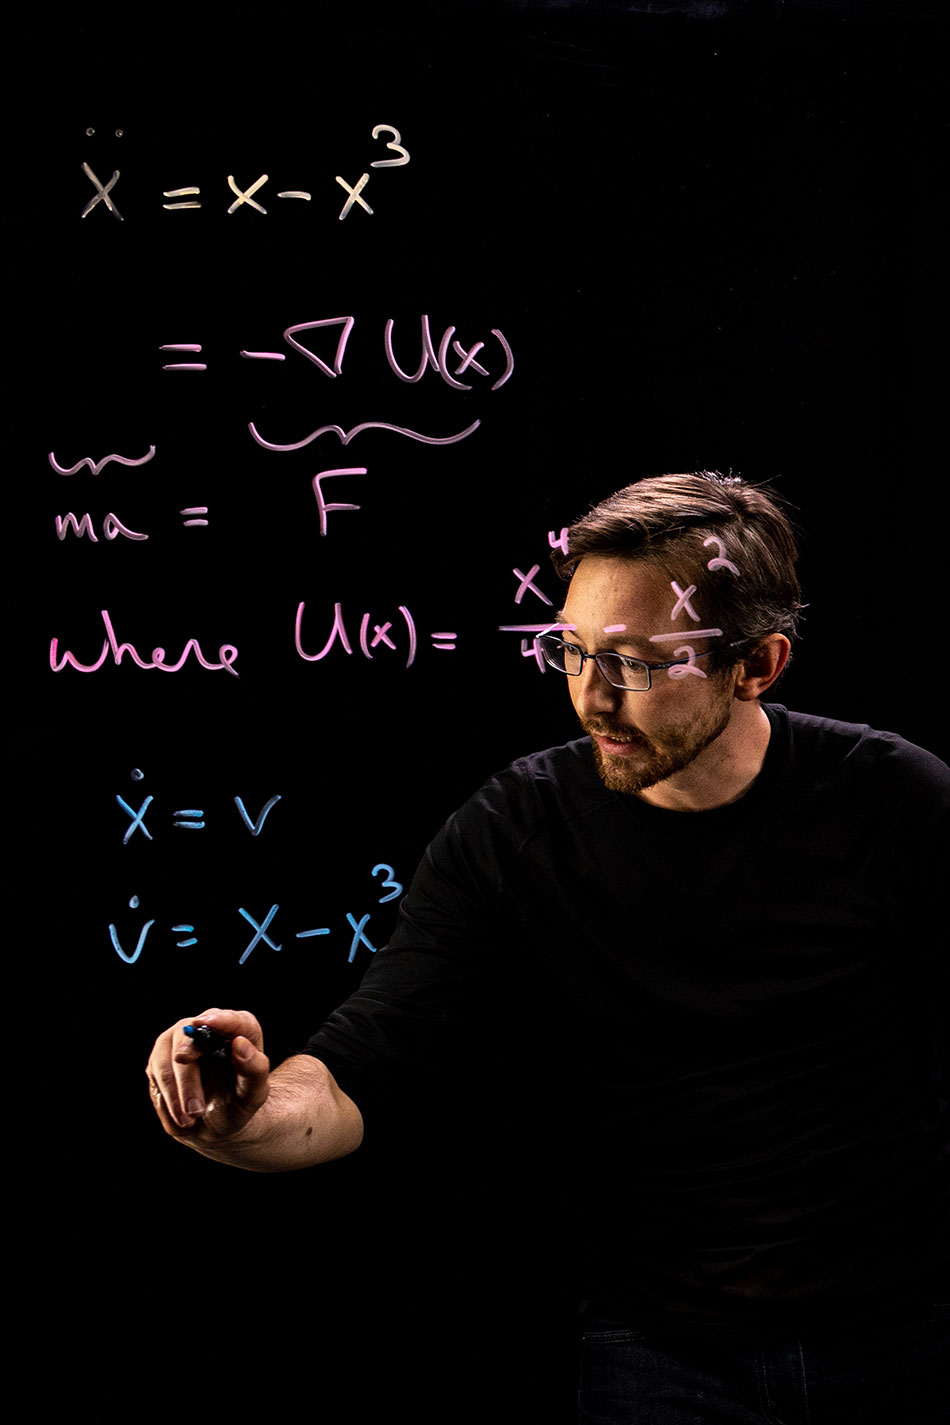
\includegraphics[height=.68\textheight]{steve}
  \end{minipage}%
  \hfill
  \begin{minipage}{.48\textwidth}
    \centering
    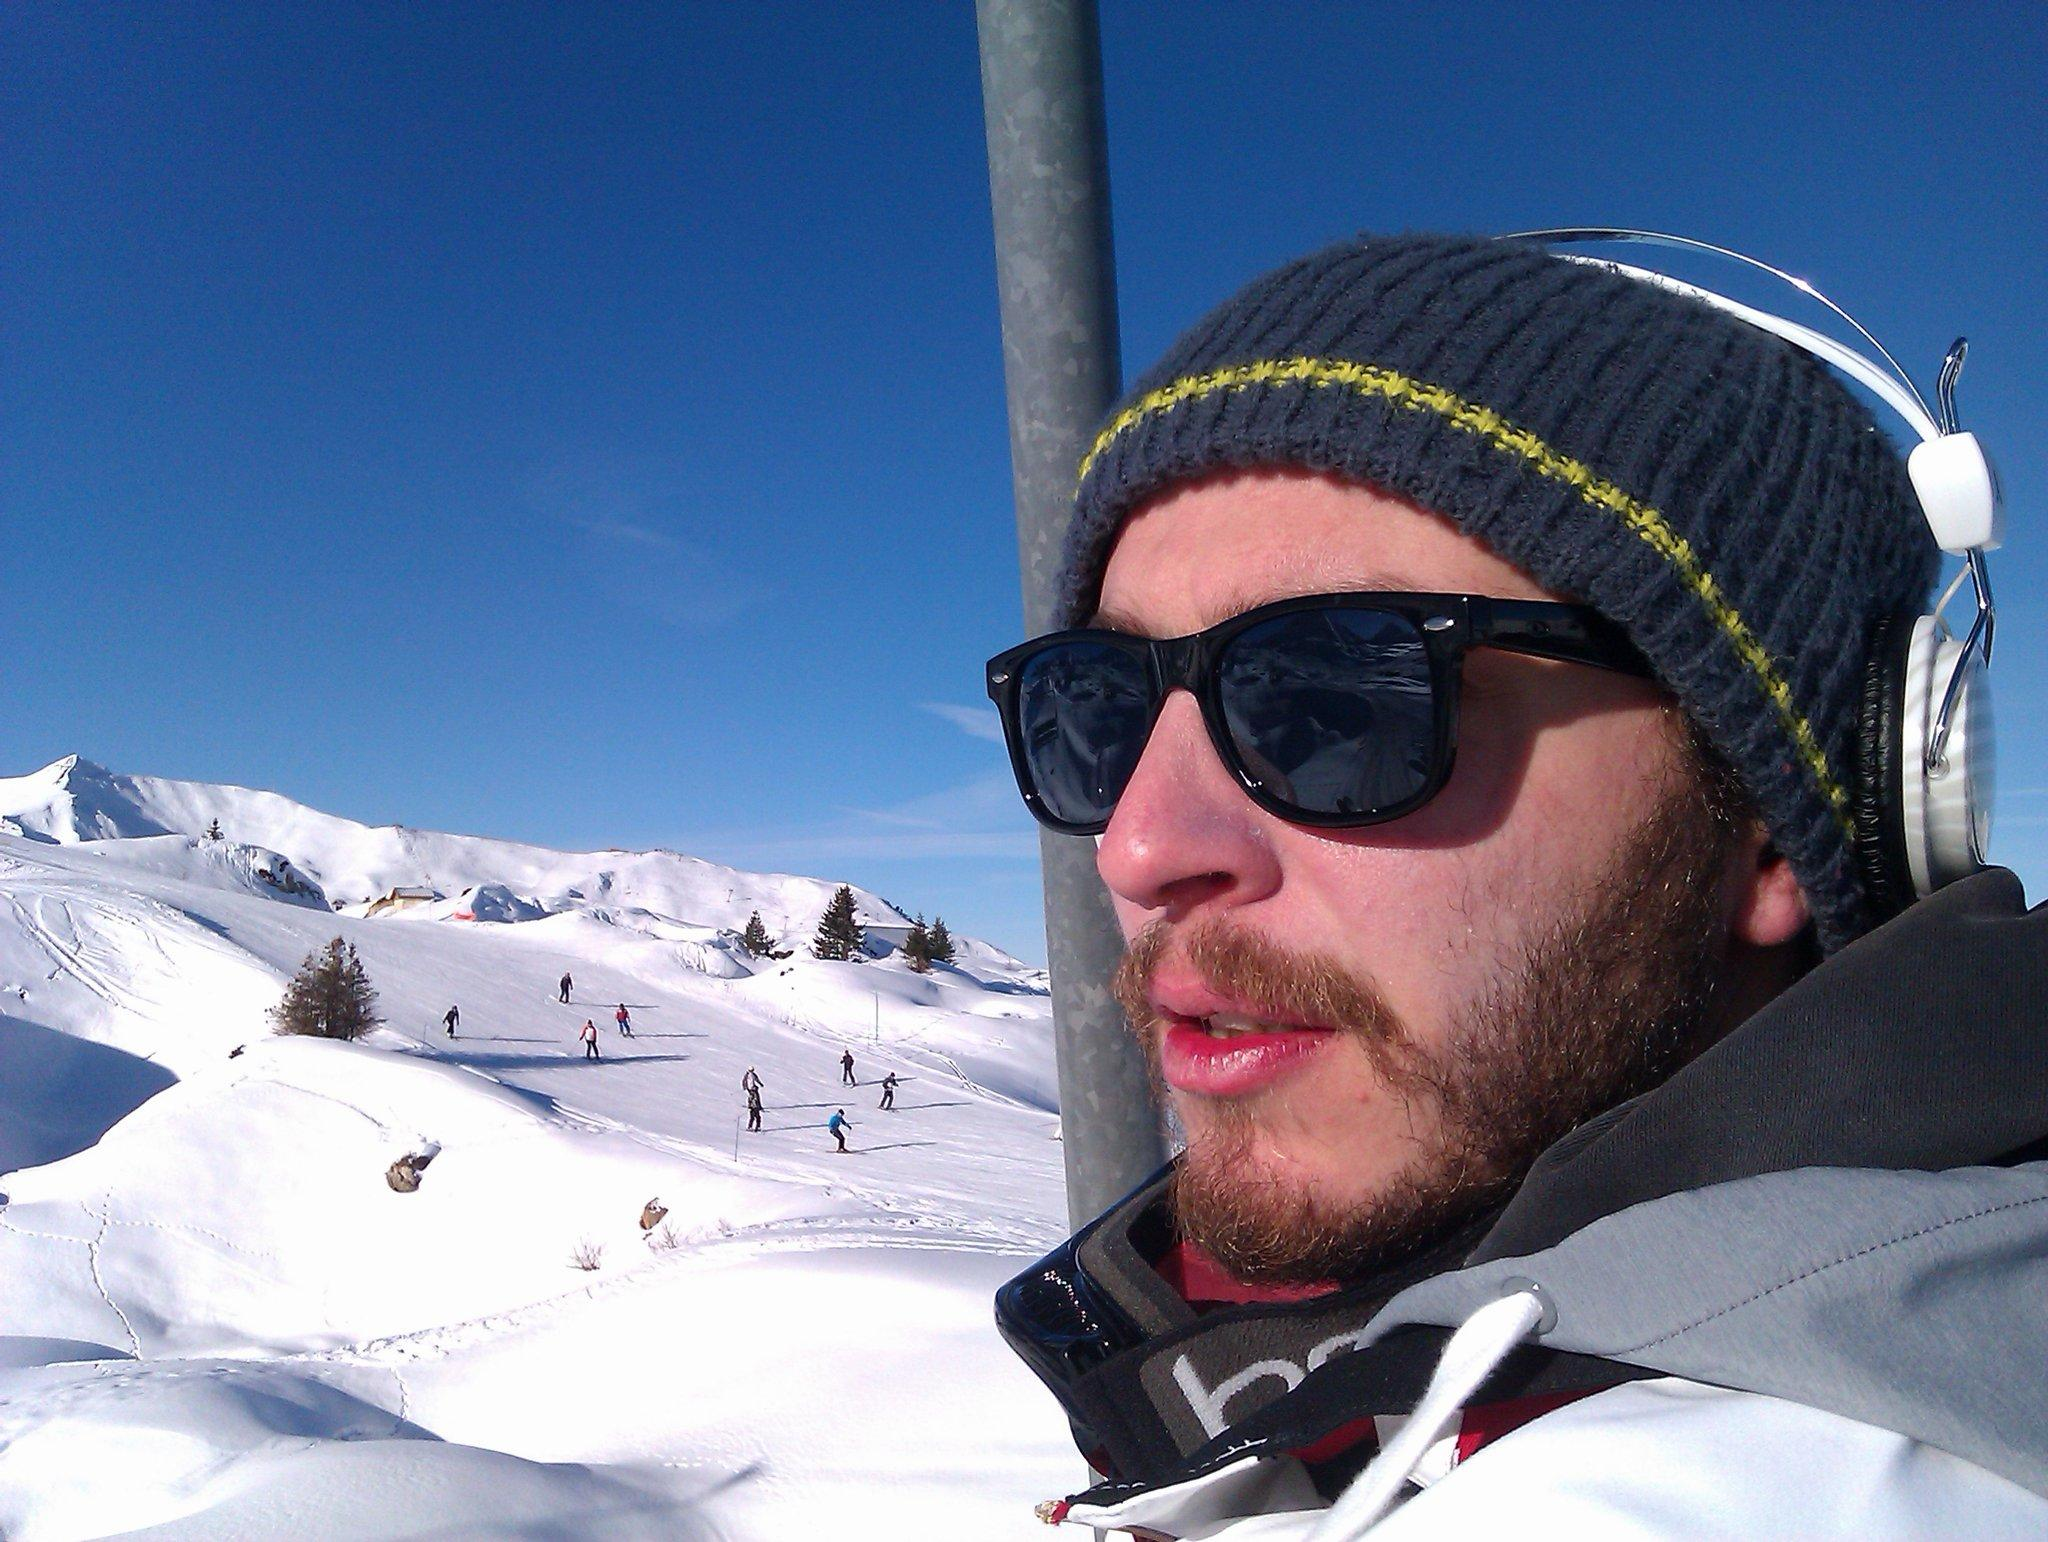
\includegraphics[width=.68\textwidth]{myself}
  \end{minipage}

  \bigskip
  \begin{minipage}{.48\textwidth}
    \centering
    \tiny
    Steve Brunton
  \end{minipage}%
  \hfill
  \begin{minipage}{.48\textwidth}
    \centering
    \tiny
    Jean-Christophe Loiseau
  \end{minipage}

  \vfill
\end{frame}

\begin{frame}
  \vfill

  \begin{minipage}{.60\textwidth}
    \vfill
    \centering
    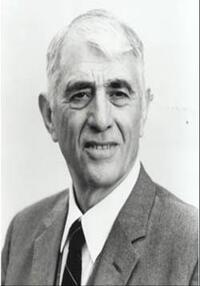
\includegraphics[width=.5\textwidth]{koopman}

    {\tiny
      Bernard Koopman (1900-1981)
    }
    \vfill
  \end{minipage}%
  \hfill
  \begin{minipage}{.36\textwidth}
    {\Large
      \textbf{
        \begin{flushright}
          Overview of Koopman theory
        \end{flushright}
      }
    }
  \end{minipage}
  
  \vfill
\end{frame}

\begin{frame}
  \vfill
  \begin{minipage}{.48\textwidth}
    \centering
    \textbf{Poincaré point of view}

    \[
      \begin{aligned}
        \vb{x}_{i+1} & = \vb{F}(\vb{x}_i, \tau) \\
        \vb{y}_{i+1} & = \vb{g}(\vb{x}_i)
      \end{aligned}
    \]
  \end{minipage}%
  \hfill
  \begin{minipage}{.48\textwidth}
    \centering
    \textbf{Koopman point of view}

    \[
      \begin{aligned}
        \mathcal{K}_{\tau} g & = g \circ \vb{F} \\
        \mathcal{K}_{\tau} g(\vb{x}_{i}) & = g(\vb{x}_{i+1})
      \end{aligned}
    \]
  \end{minipage}
  \vfill
\end{frame}

\begin{frame}
  \vfill
  {
    \Large
    \[
      \mathcal{K}_{\tau} \left(  \alpha g_1 + \beta g_2 \right) = \left( \alpha g_1 + \beta g_2 \right) \circ \vb{F}
    \]

    \[
      \Updownarrow
    \]

    \[
      \alpha \mathcal{K}_{\tau} g_1 + \beta \mathcal{K} g_2 = \alpha g_1 \circ \vb{F} + \beta g_2 \circ \vb{F}
    \]
  }
  \vfill
\end{frame}

\begin{frame}
  \vfill
  \centering

  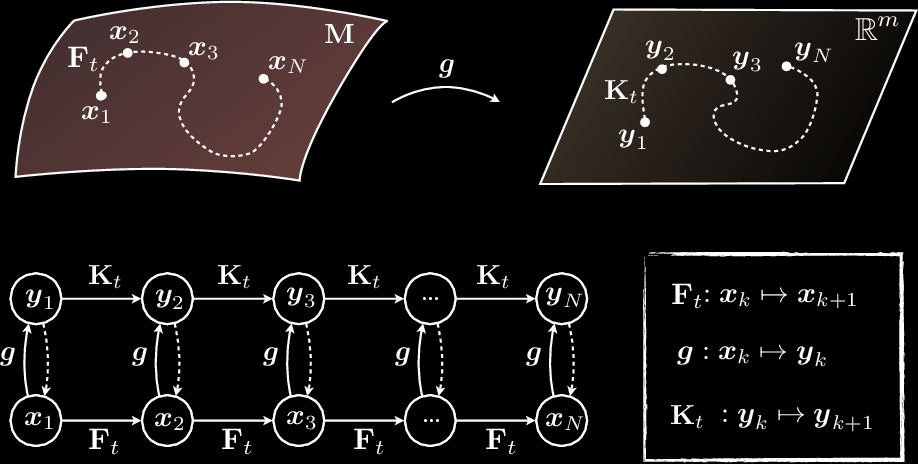
\includegraphics[width=\textwidth]{koopman_operator}
  
  \vfill
\end{frame}

\begin{frame}
  \vfill
  {
    \Large
    \[
      \norm{ \hat{\mathcal{K}} - \mathcal{K} }_{HS}^2 = \norm{ \hat{\mathcal{K}} }_{HS}^2 - 2 \langle \hat{\mathcal{K}} \vert \mathcal{K} \rangle_{HS} + \norm{ \mathcal{K} }_{HS}^2
    \]
  }
  \vfill
\end{frame}

\begin{frame}
  \vfill
  Let $f_i$, $g_i$ and $\hat{\sigma}_i$ be the i\textsuperscript{th} singular triplet of $\hat{\mathcal{K}}$.
  We can then write

  {
    \Large
    \[
      \norm{\hat{\mathcal{K}} - \mathcal{K}}_{HS}^2 = \sum_{i=1}^r \hat{\sigma}_i^2 \langle f_i \vert f_i \rangle_{\rho_1} \langle g_i \vert g_i \rangle_{\rho_0} - 2 \sum_{i=1}^r \hat{\sigma}_i \langle f_i \vert \mathcal{K} g_i \rangle + \sum_{j=1}^{\infty} \sigma_j^2
    \]
  }
  \vfill
\end{frame}

\begin{frame}
  \vfill
  {
    \Large
    \[
      \norm{ \hat{\mathcal{K}} - \mathcal{K} }_{HS}^2 = -\tikzmarknode{a}{\highlightdark{blue}{\mathcal{R}_E(\hat{\sigma}, f, g)}} + \norm{ \mathcal{K} }_{HS}^2
    \]
  }

  \begin{tikzpicture}[overlay, remember picture, >=stealth, nodes={align=left, inner ysep=1pt}, <-]
    \path (a.north) ++ (0, 2em) node[anchor=south east, color=blue!67] (dynamics){Maximize this score based on data};
    \draw [color=blue!87] (a.north) |- ([xshift=0.3ex, color=blue] dynamics.south west);
  \end{tikzpicture}
 
  \vfill
\end{frame}

\begin{frame}
  \vfill
  Let $\boldsymbol{\chi}_0 = \rowvec{\chi_0^{(1)}, \chi_0^{(2)}, \chi_0^{(3)}, \cdots}^T$ be an arbitrary basis for the input space $\mathcal{L}_0^2$, and let $\vb{g} = \vb{V}^T \boldsymbol{\chi}_0$ be an orthonormal basis for this space.
  It must then satisfy

  \vfill
  
  {
    \Large
    \[
      \langle g_i \vert g_j \rangle_{\rho_0} = \vb{v}_i^T \vb{C}_{00} \vb{v}_j = \delta_{ij}
    \]
  }

  \vfill
  
  with $\vb{C}_{00} = \mathbb{E} \left[ \boldsymbol{\chi}_0(\vb{x}_t) \boldsymbol{\chi_0}(\vb{x}_t)^T \right]$.
  A similar expression applies for $f$ with basis $\boldsymbol{\chi}_1$ and density $\rho_1$.
  \vfill
\end{frame}

\begin{frame}
  \vfill

  After some algebraic manipulations, we arrive at

  \vfill
  
  {
    \Large
    \[
      \begin{aligned}
        \maximize_{\vb{U}, \vb{V}} & \quad \trace{ \vb{U}^T \vb{C}_{10} \vb{V} } \\
        \subto & \quad \vb{U}^T \vb{C}_{11} \vb{U} = \vb{I}_r \\
               & \quad \vb{V}^T \vb{C}_{00} \vb{V} = \vb{I}_r
      \end{aligned}
    \]
  }

  \vfill

  with $\vb{C}_{10} = \mathbb{E} \left[ \boldsymbol{\chi}_1(\vb{x}_t) \boldsymbol{\chi}_0(\vb{x}_{t+\tau}) \right]$.
  \vfill
\end{frame}

\begin{frame}
  \vfill

  \begin{enumerate}
  \item Compute the covariance matrices $\vb{C}_{00}$, $\vb{C}_{11}$, and $\vb{C}_{10}$.
    \bigskip
  \item Perform the truncated SVD
    % 
    \[
      \vb{C}_{11}^{-\frac12} \vb{C}_{10} \vb{C}_{00}^{-\frac12} = \vb{U}^{\prime} \vb{K} \vb{V}^{\prime T}
    \]

    \medskip
  \item Compute $\vb{U} = \vb{C}_{11}^{-\frac12} \vb{U}^{\prime}$ and $\vb{V} = \vb{C}_{00}^{-\frac12} \vb{V}^{\prime}$.
    \bigskip
  \item Output the singular values $K_{ii}$ and singular functions $f_i = \vb{u}_i^T \boldsymbol{\chi}_1$ and $g_i = \vb{v}_i^T \boldsymbol{\chi}_0$.
  \end{enumerate}

  \vfill
\end{frame}
{
  \setbeamercolor*{background canvas}{bg=white}
  \setbeamercolor{normal text}{fg=black}
  \usebeamercolor[fg]{normal text}

  \begin{frame}
    \vfill
    \centering
    \textbf{Orstein-Uhlenbeck process}
    {
      \Large
      \[
        \dd \vb{x}_t = \vb{A} \vb{x}_t \ \dd t + \vb{B} \ \dd \vb{w}_t
      \]
    }
    \vfill
  \end{frame}

  \begin{frame}
    \vfill
    \centering
    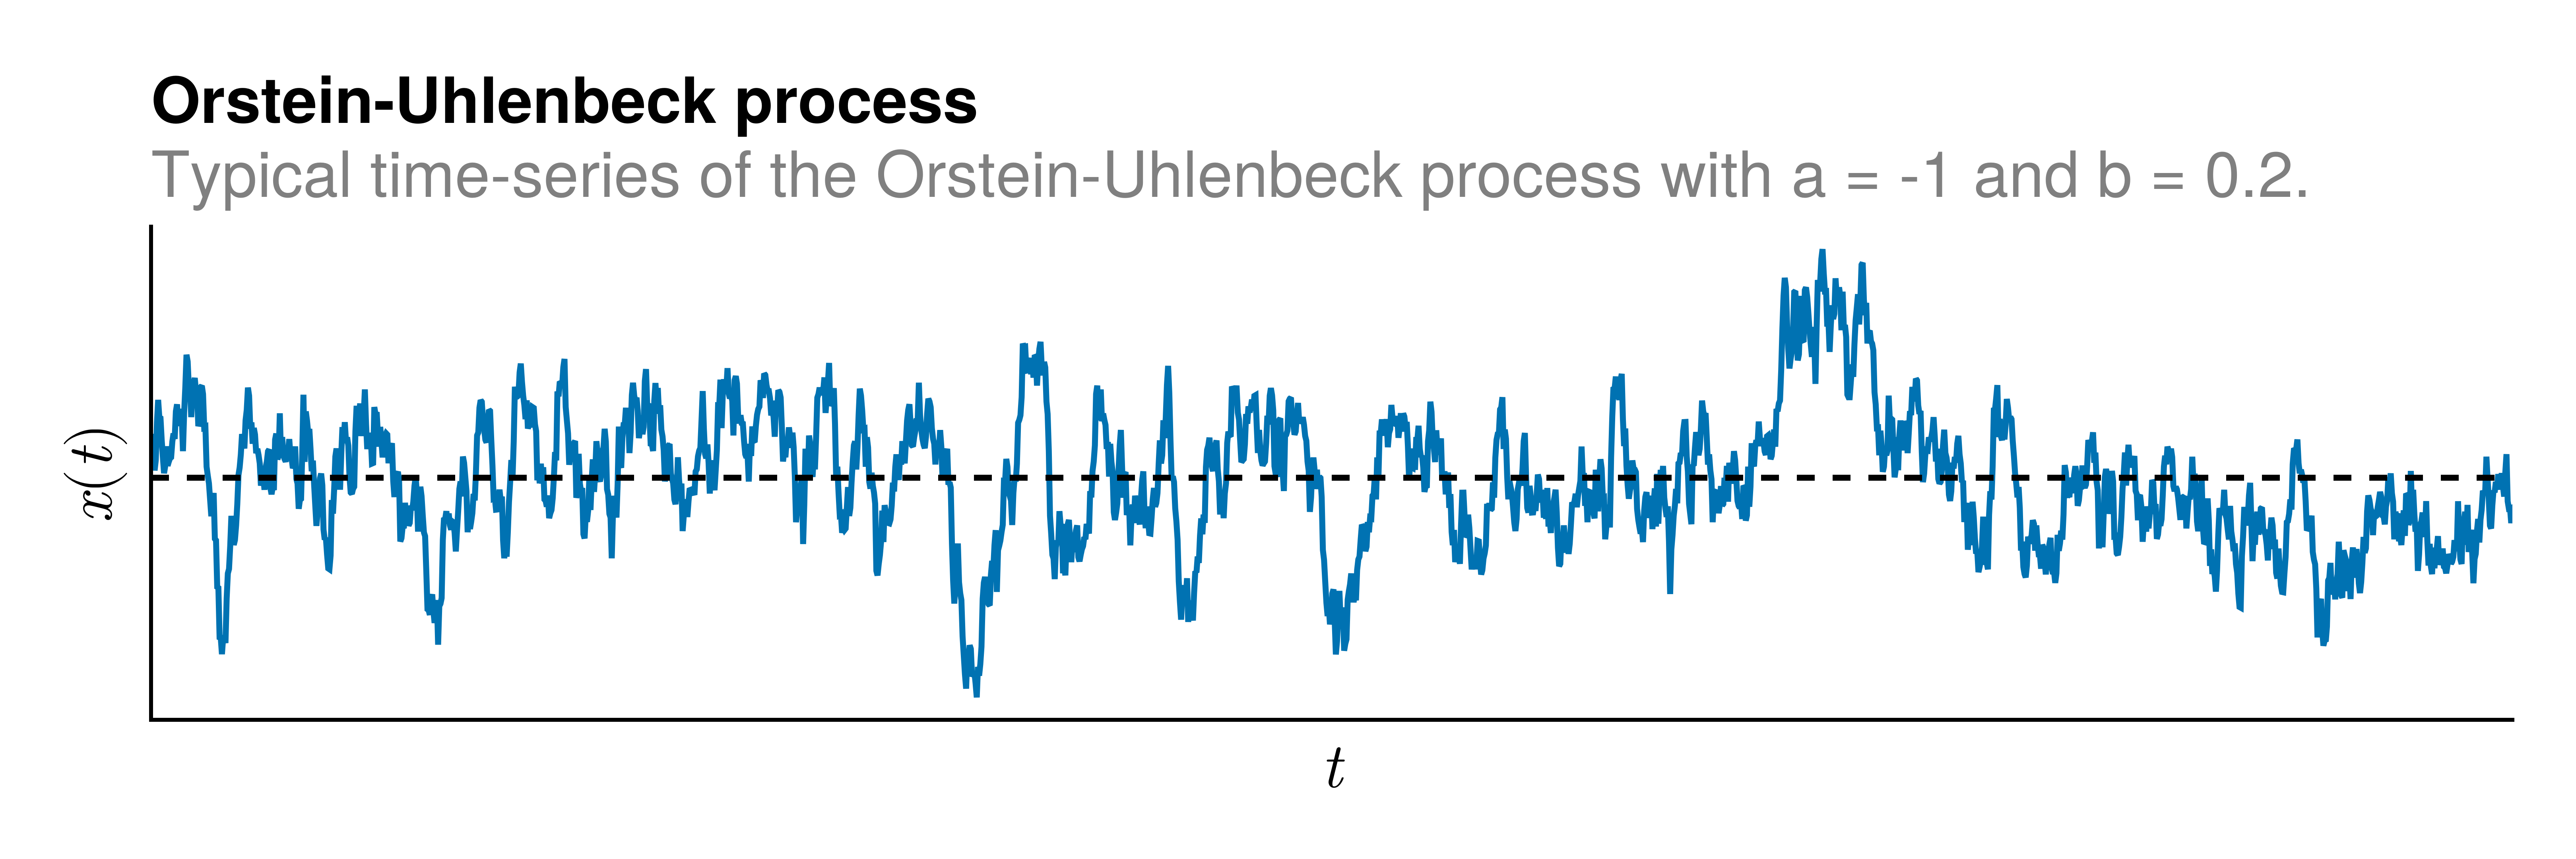
\includegraphics[width=\textwidth]{OU_process}
    \vfill
  \end{frame}

  \begin{frame}
    \vfill
    \begin{minipage}{.48\textwidth}
      Given an ergodic time-series, use
      %
      \[
        \chi_0 = \chi_1 = \rowvec{1, x, x^2, x^3, \cdots}^T
      \]
      %
      to approximate the Koopman singular functions.
    \end{minipage}%
    \hfill
    \begin{minipage}{.48\textwidth}
      \centering
      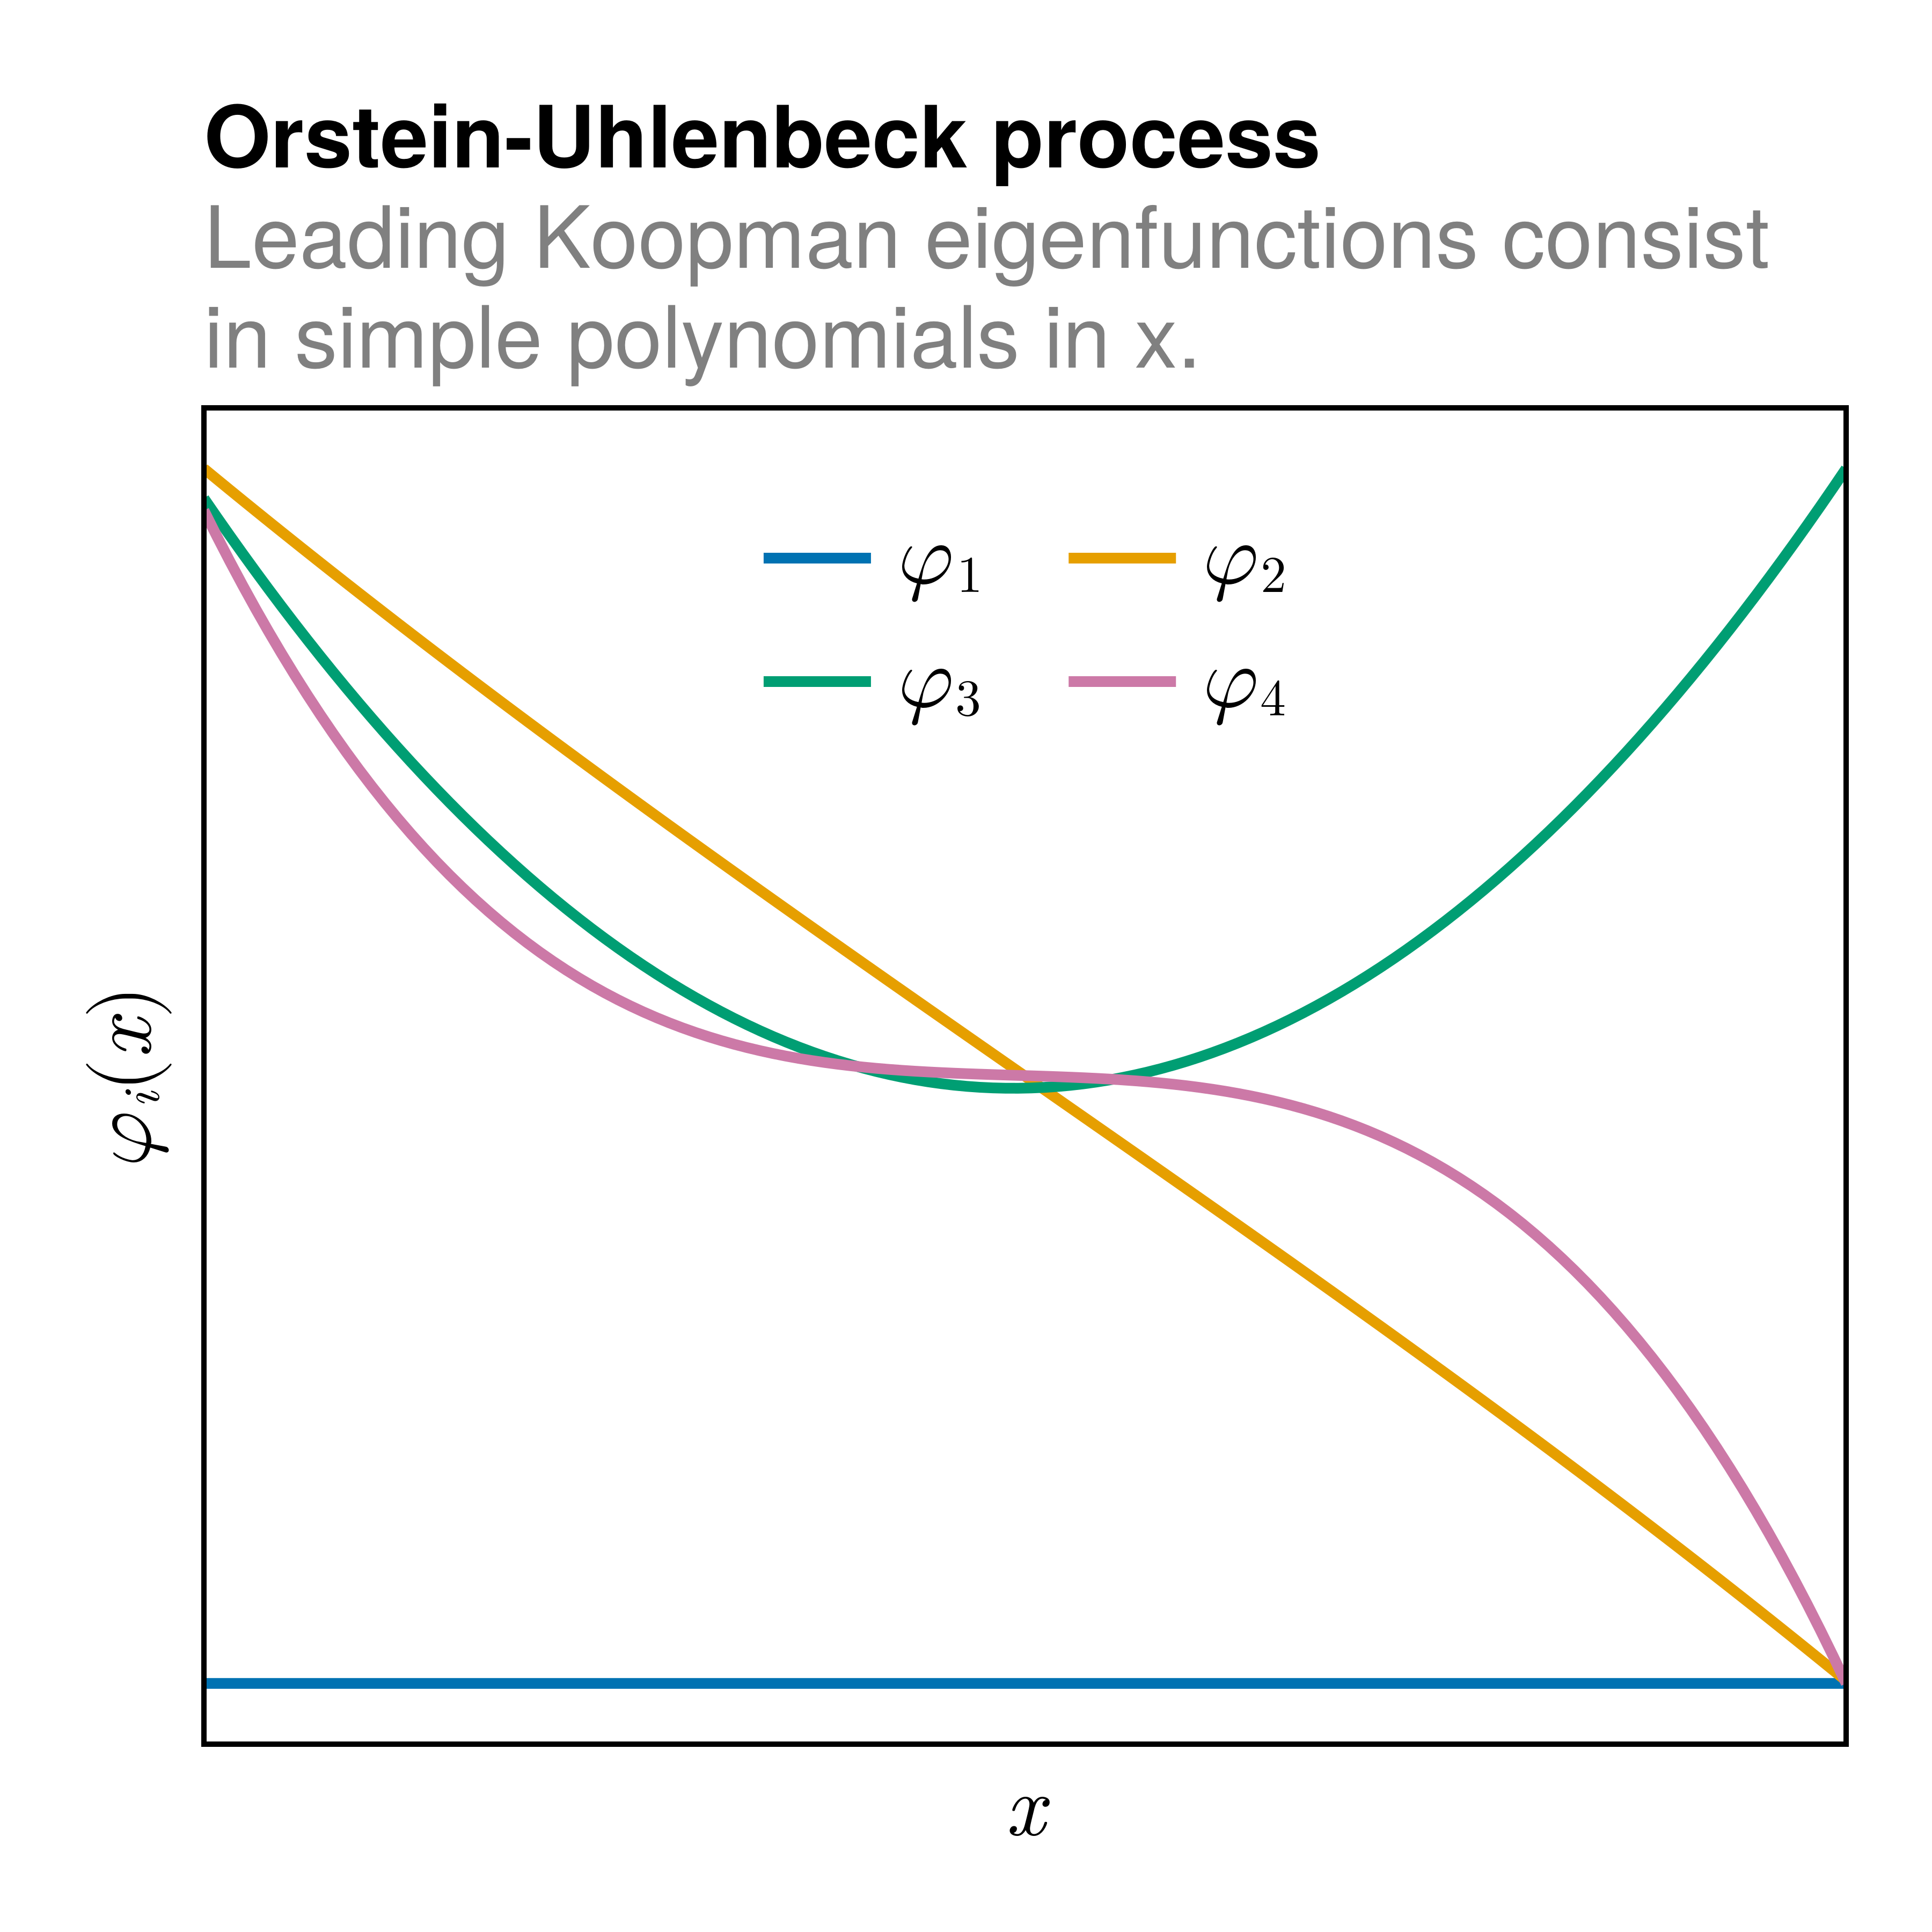
\includegraphics[width=\textwidth]{OU_process_eigenfunctions}
    \end{minipage}
    \vfill
  \end{frame}

  \begin{frame}
    \vfill
    \begin{minipage}{.48\textwidth}
      Use the VAMP-E score $\mathcal{R}_e(p)$ for cross-validation purposes.

      \bigskip
      
      For the OU process, setting $p > 3$ is unecessary.
    \end{minipage}%
    \hfill
    \begin{minipage}{.48\textwidth}
      \centering
      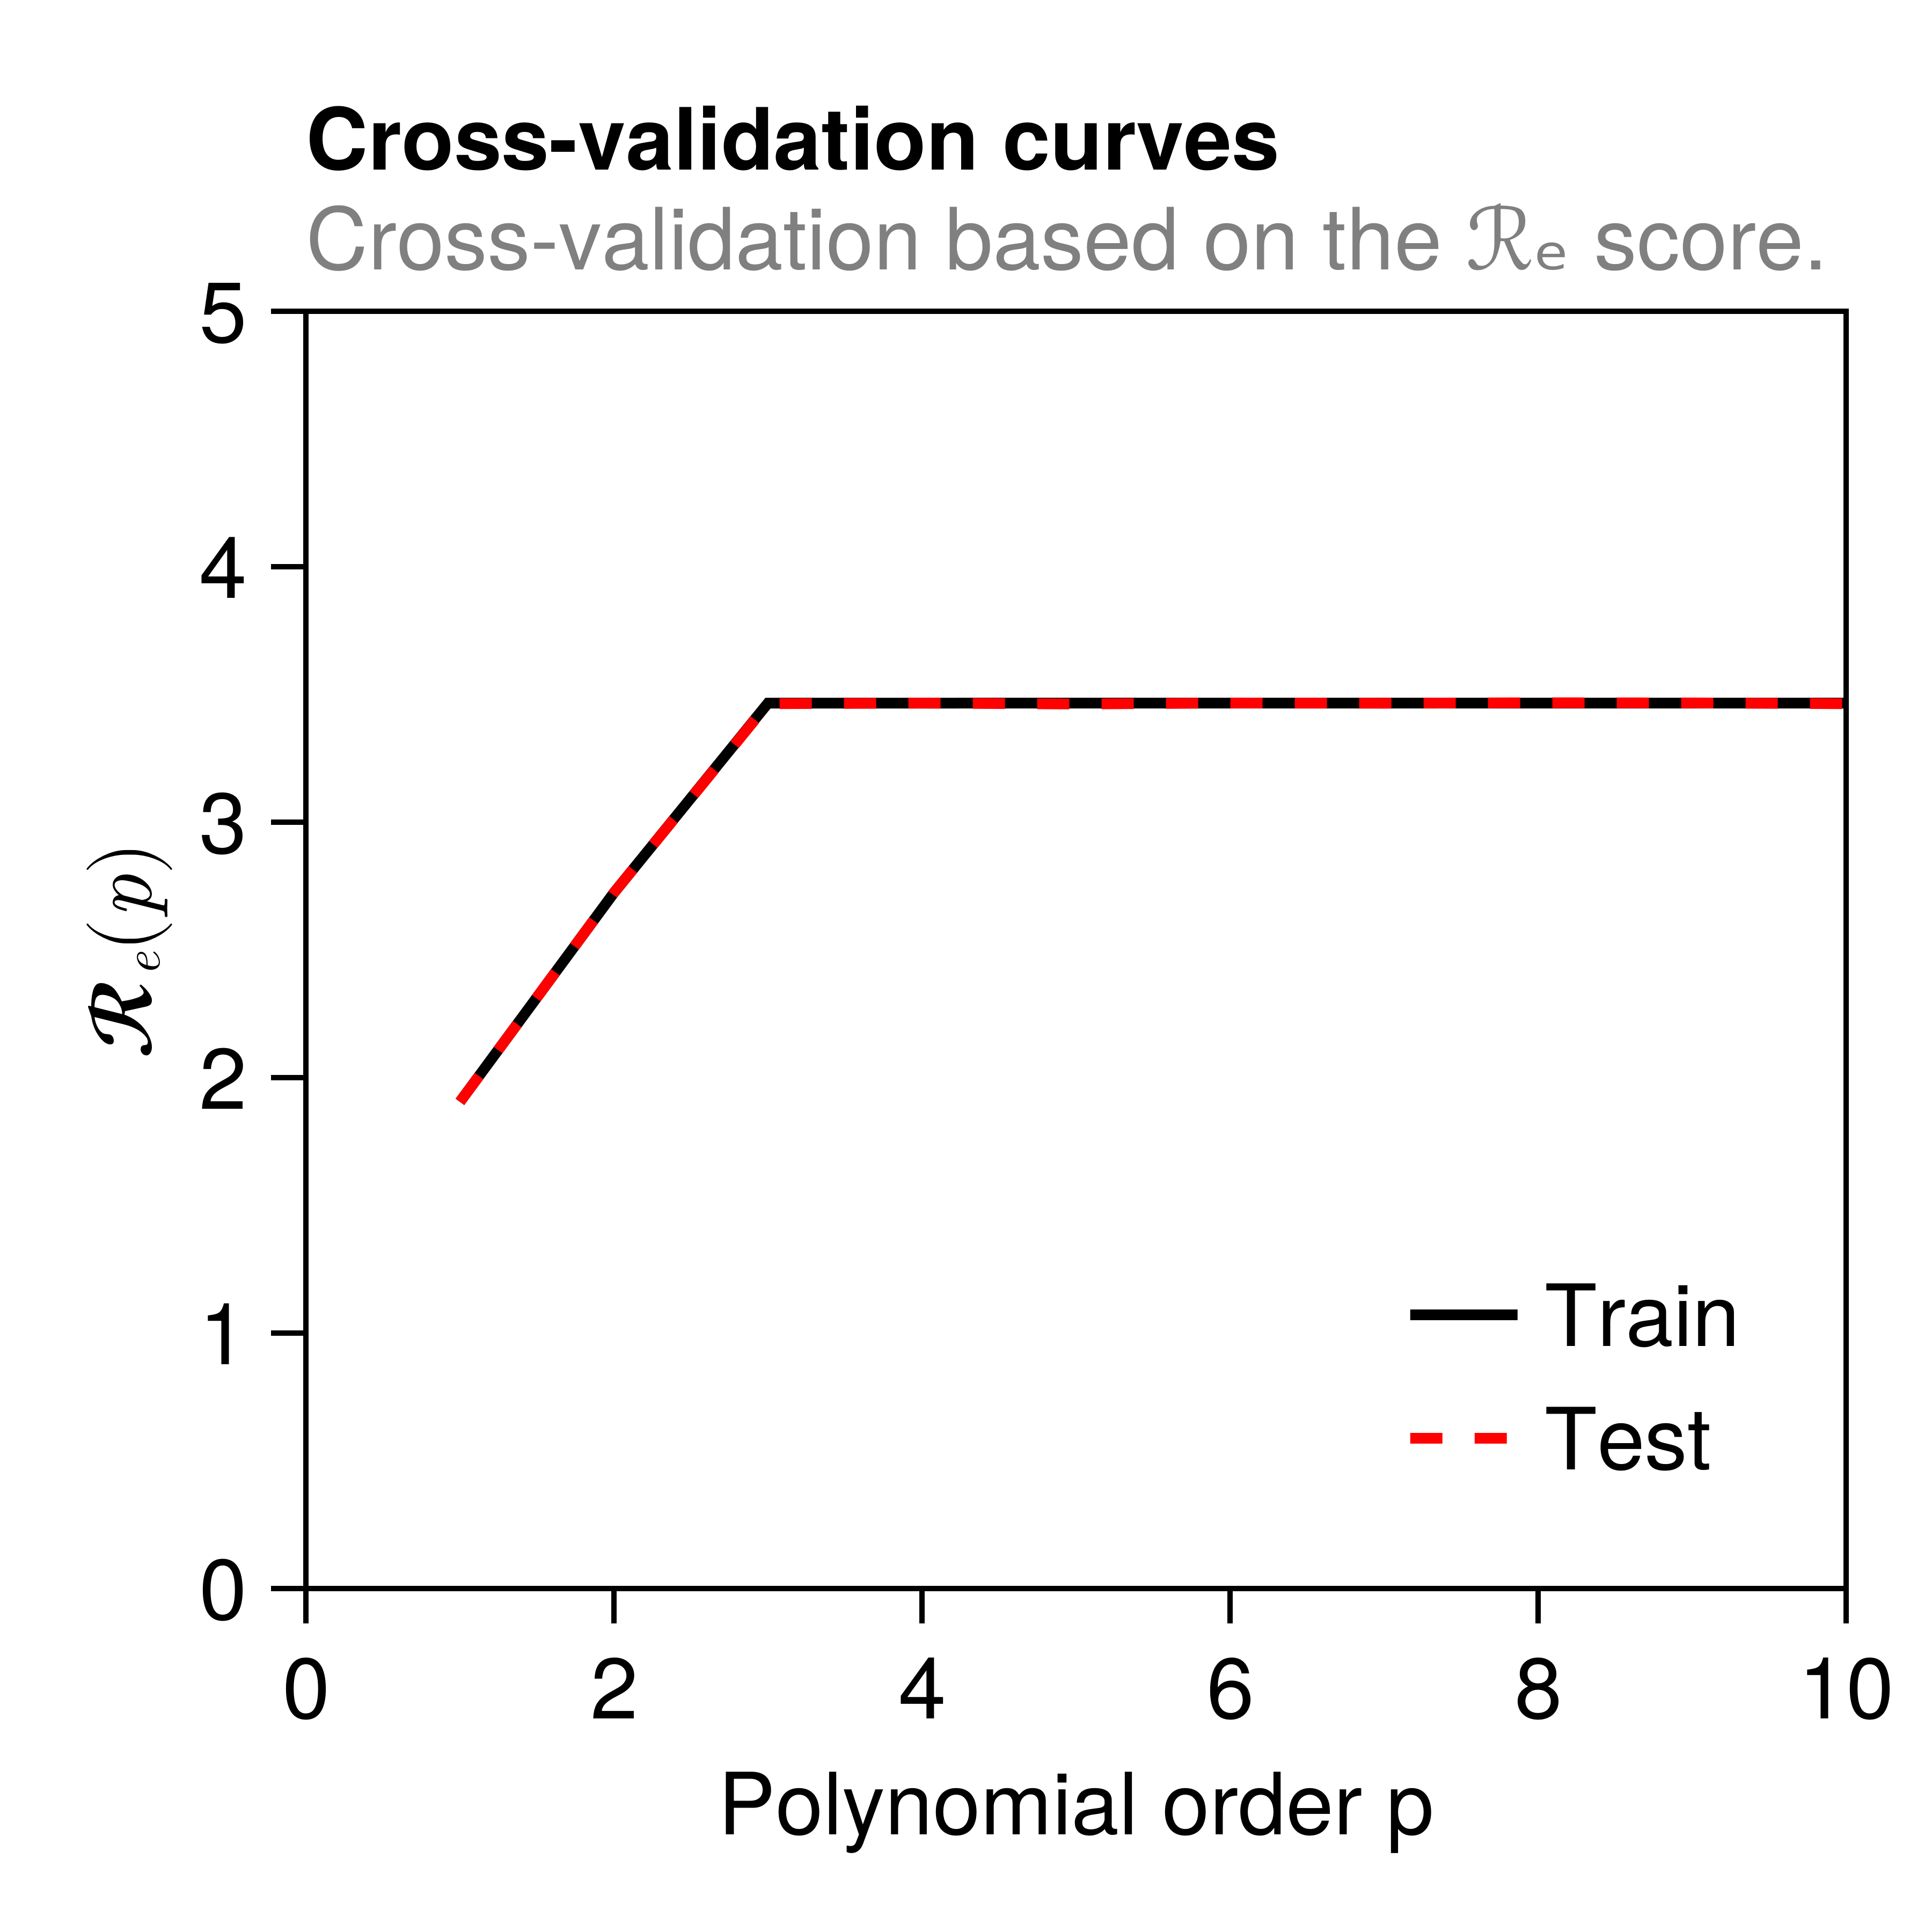
\includegraphics[width=\textwidth]{OU_process_cross_validation}
    \end{minipage}
    \vfill
  \end{frame}

  \begin{frame}
    \vfill
    \begin{minipage}{.48\textwidth}
      $\mathcal{R}_e$ can also be used to check convergence w.r.t the size of the dataset.

      \bigskip

      For the OU process, a few thousands samples are sufficient.
    \end{minipage}%
    \hfill
    \begin{minipage}{.48\textwidth}
      \centering
      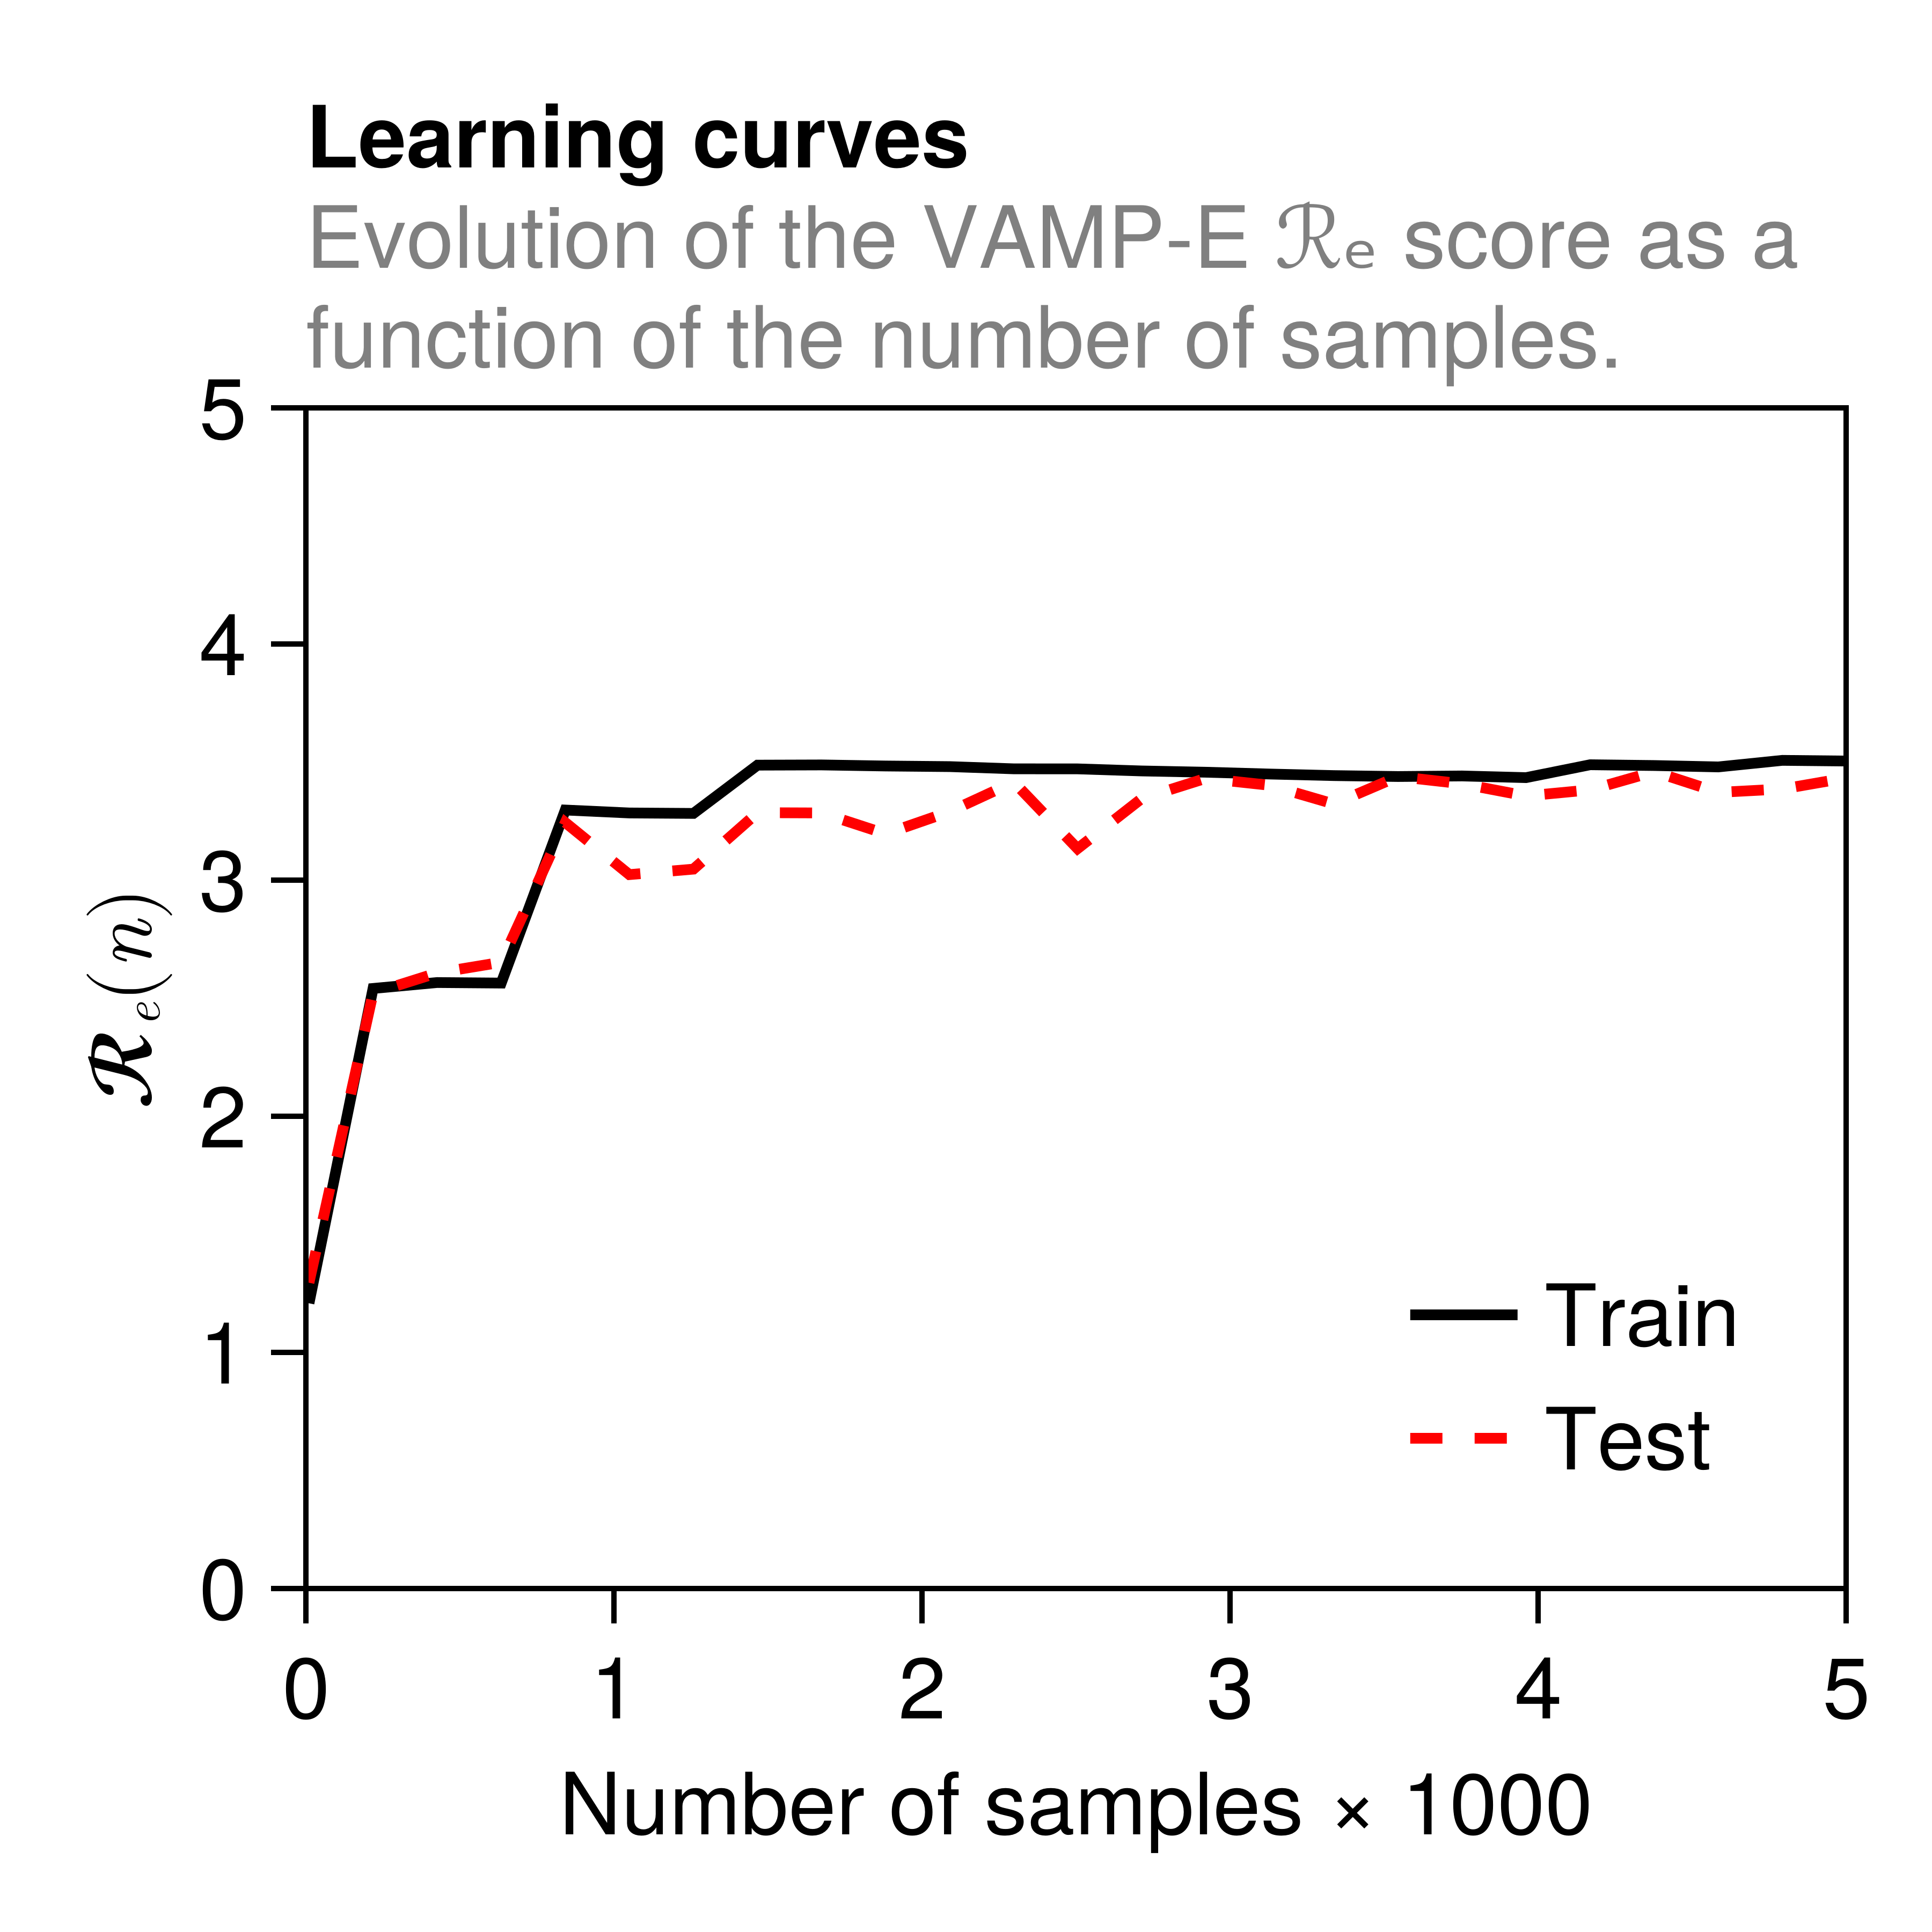
\includegraphics[width=\textwidth]{OU_process_learning_curve}
    \end{minipage}
    \vfill
  \end{frame}

  \begin{frame}
    \vfill
    \begin{minipage}{.48\textwidth}
      \centering
      \textbf{Lorenz system}

      {
        \Large
        \[
          \begin{aligned}
            \dot{x} & = \sigma \left( y - x \right) \\
            \dot{y} & = x \left( \rho - z \right) - y \\
            \dot{z} & = xy - \beta z
          \end{aligned}
        \]
      }
    \end{minipage}%
    \hfill
    \begin{minipage}{.48\textwidth}
      \centering
      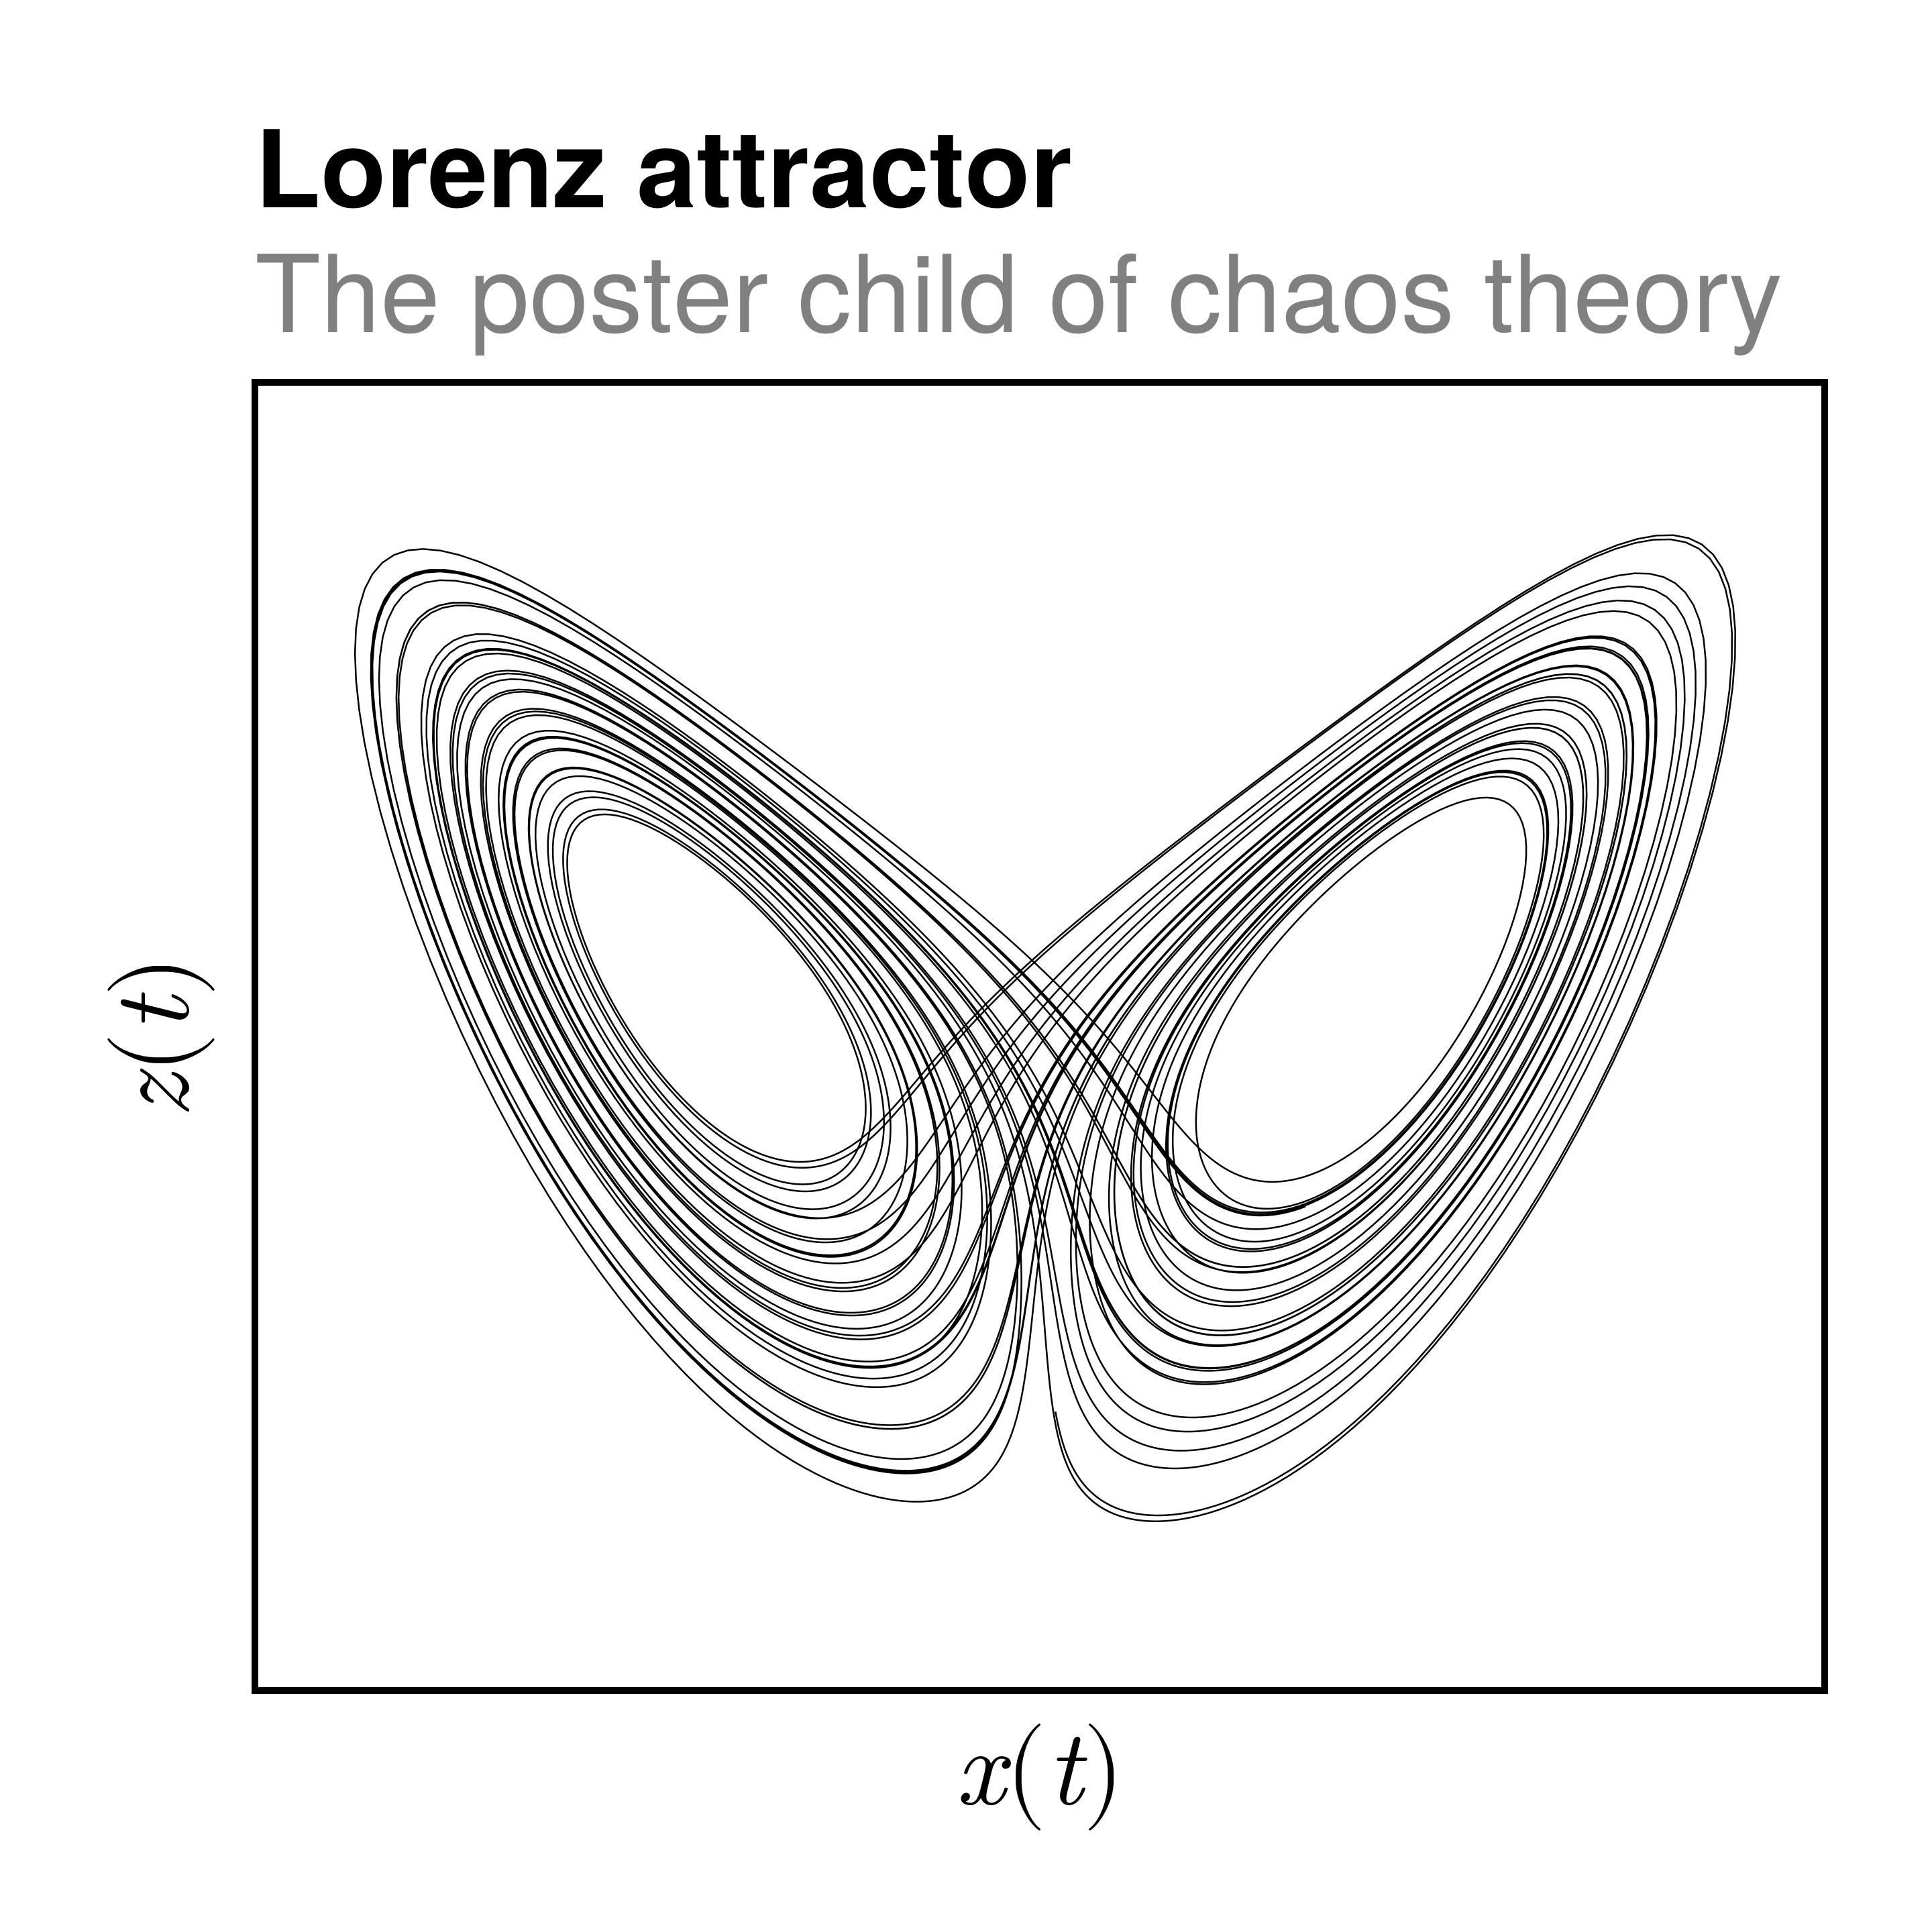
\includegraphics[width=\textwidth]{Lorenz_attractor}
    \end{minipage}
    \vfill
  \end{frame}

  \begin{frame}
    \vfill
    \begin{minipage}{.48\textwidth}
      Given an ergodic time-series, use
      %
      \[
        \chi = \rowvec{x, y, z, x^2, xy, xz, y^2, \cdots}^T
      \]
      %
      to approximate the Koopman singular functions.
    \end{minipage}%
    \hfill
    \begin{minipage}{.48\textwidth}
      \centering
      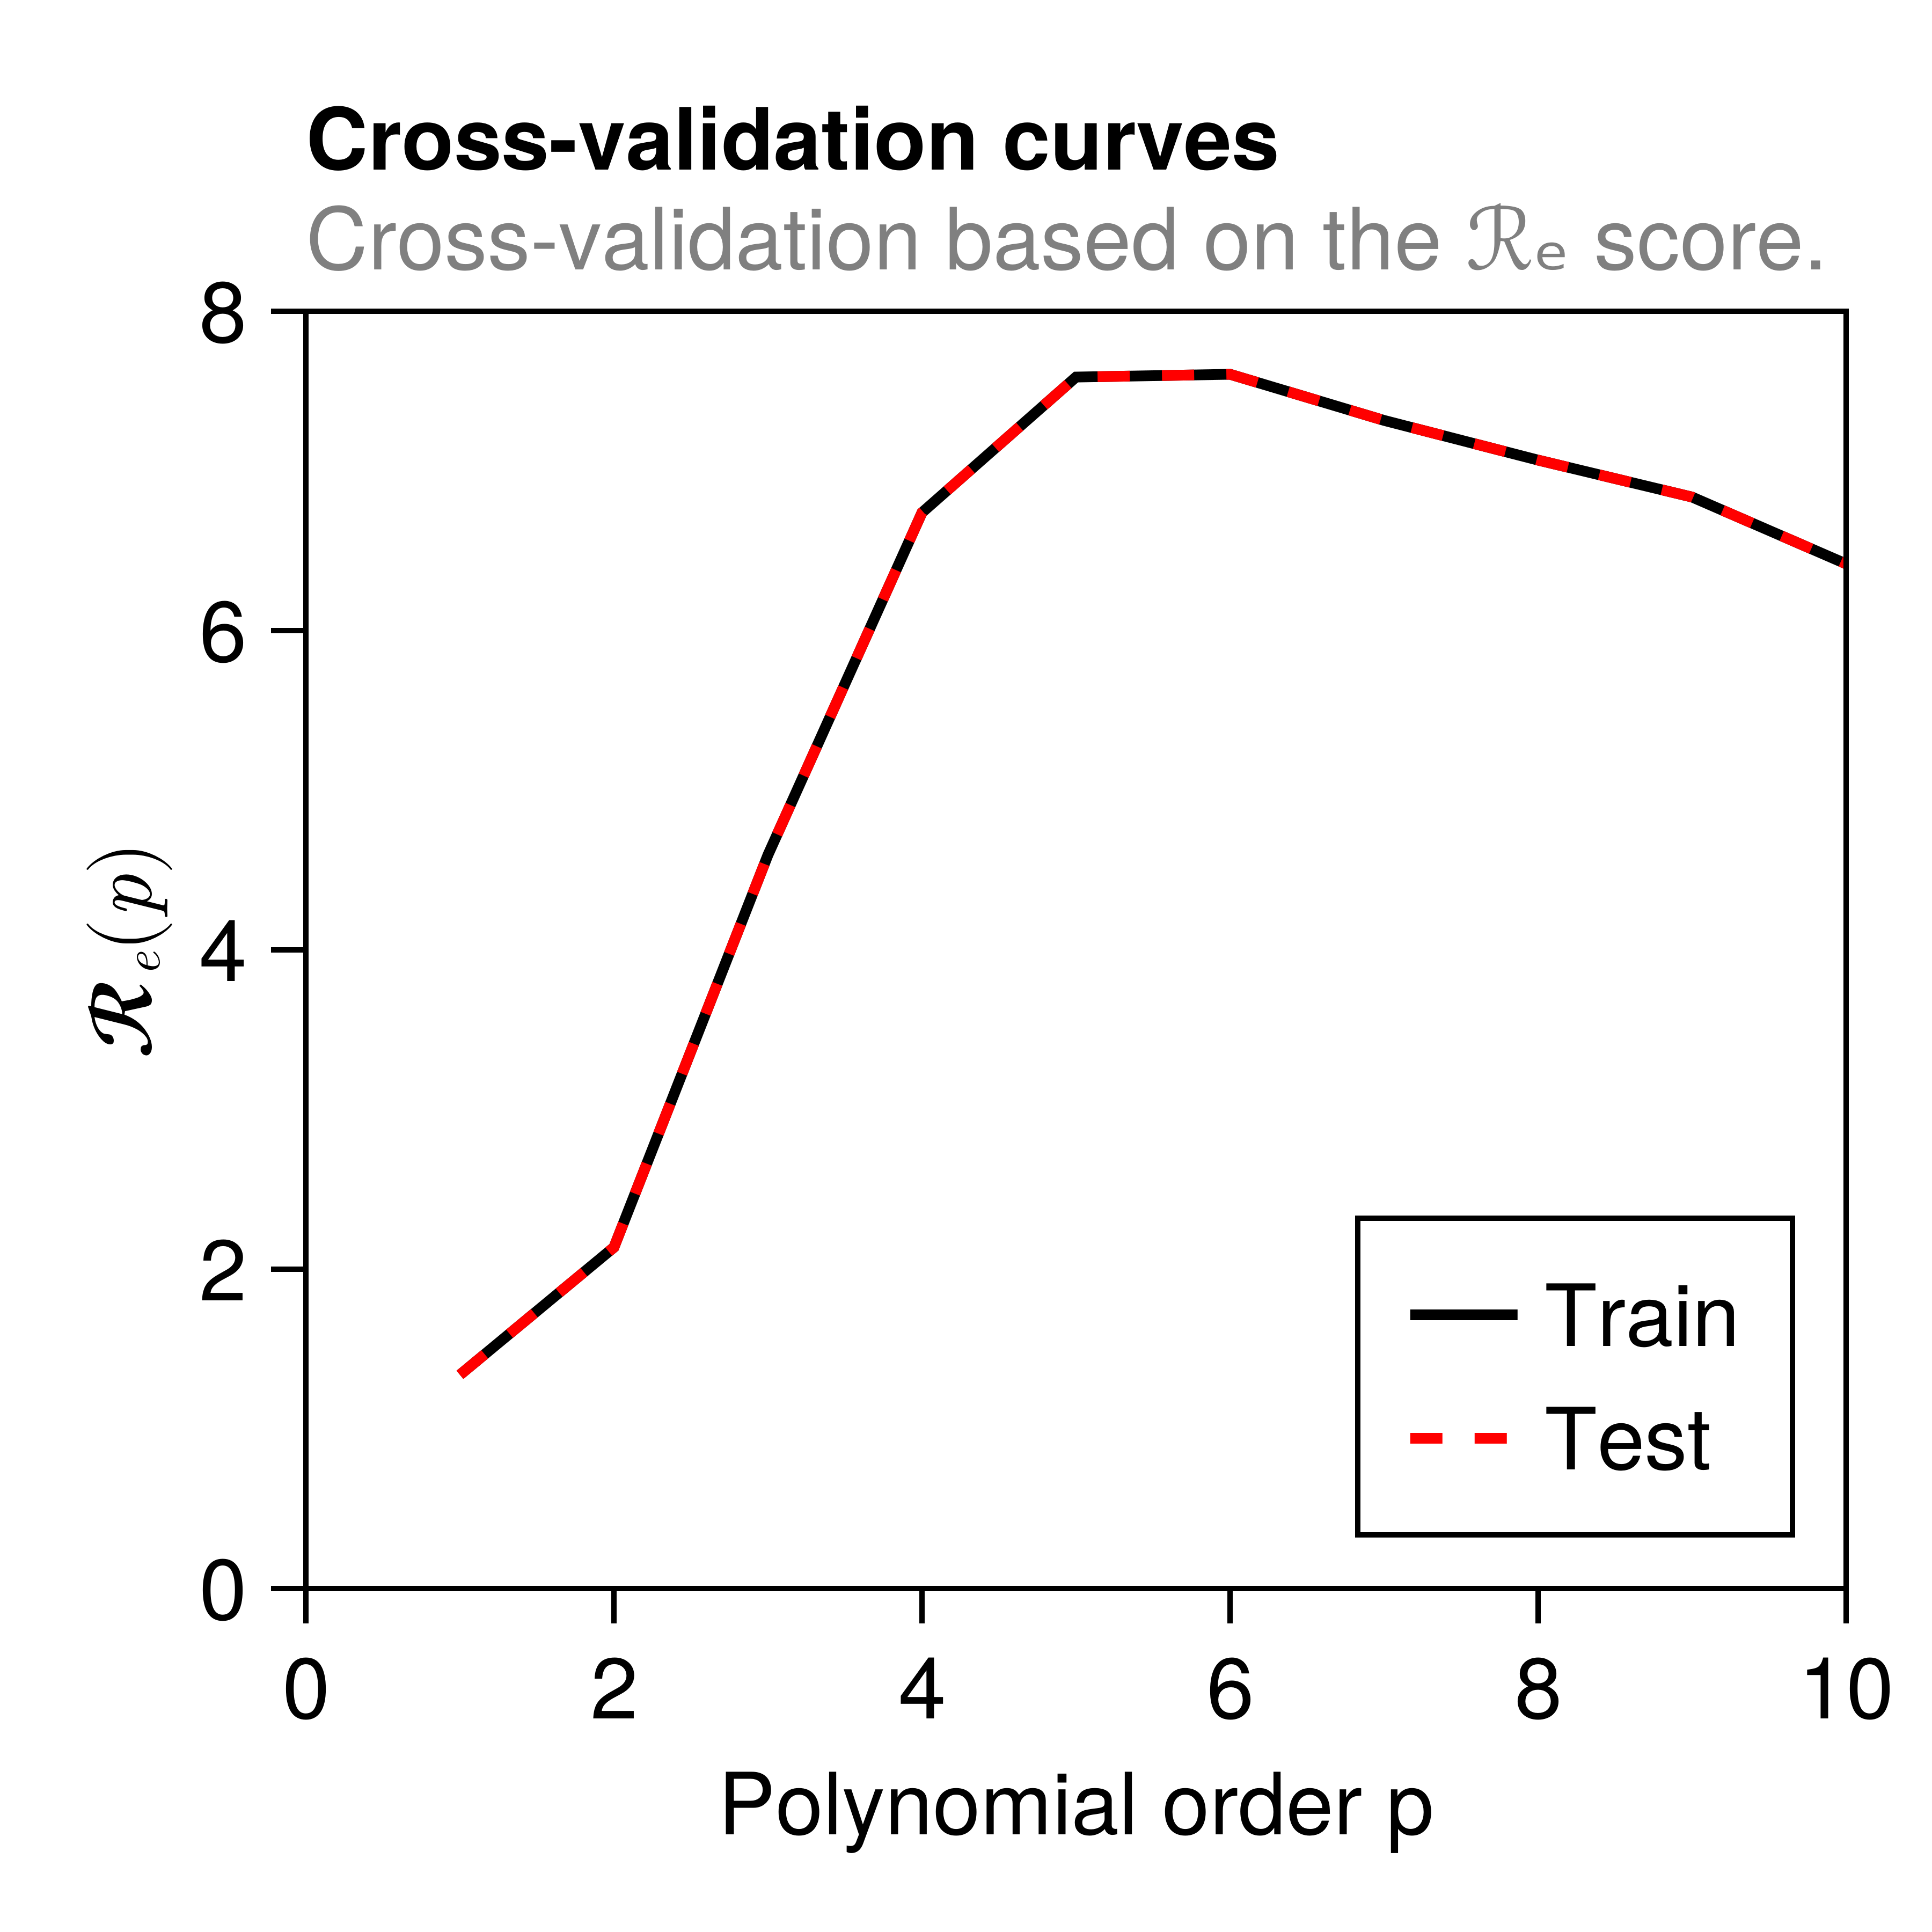
\includegraphics[width=\textwidth]{Lorenz_cross_validation}
    \end{minipage}
    \vfill
  \end{frame}

  \begin{frame}
    \vfill
    \begin{center}
      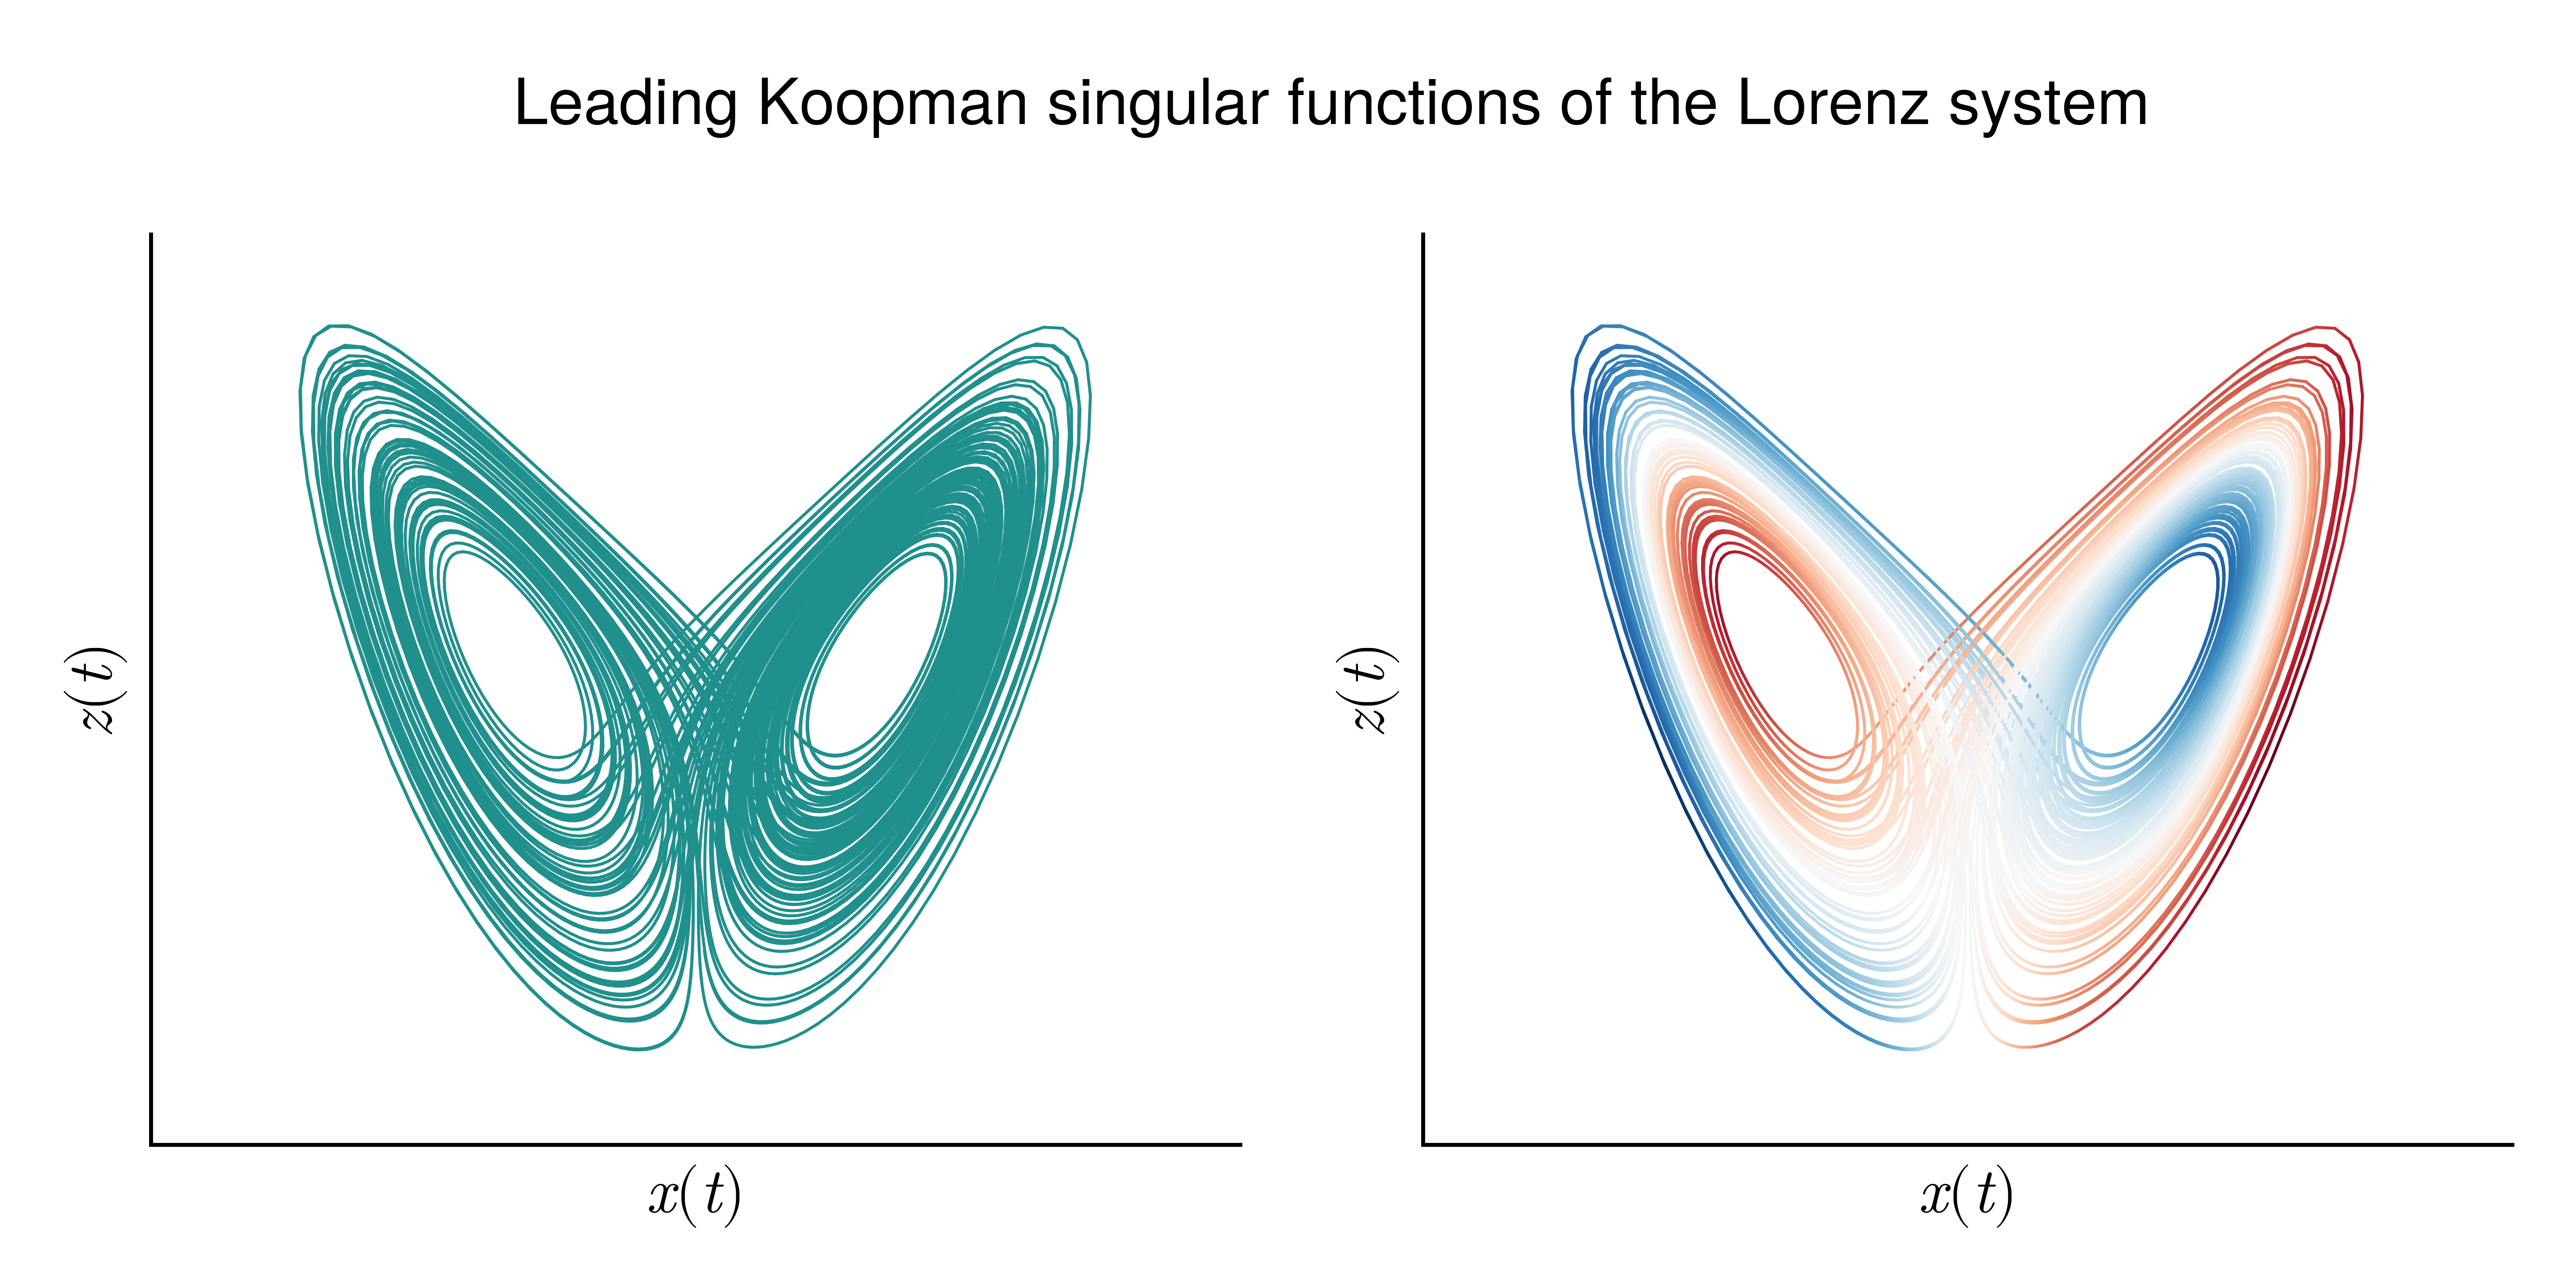
\includegraphics[width=.8\textwidth]{Lorenz_eigenfunctions}
    \end{center}

    The leading non-trivial Koopman singular function partitions the state space into metastable (almost-invariants) sets.
    \vfill
  \end{frame}

  \begin{frame}
    \vfill
    \begin{minipage}{.48\textwidth}
      If a single time-series is available, use Takens theorem and time-delay embedding to reconstruct the attractor.
    \end{minipage}%
    \hfill
    \begin{minipage}{.48\textwidth}
      \centering
      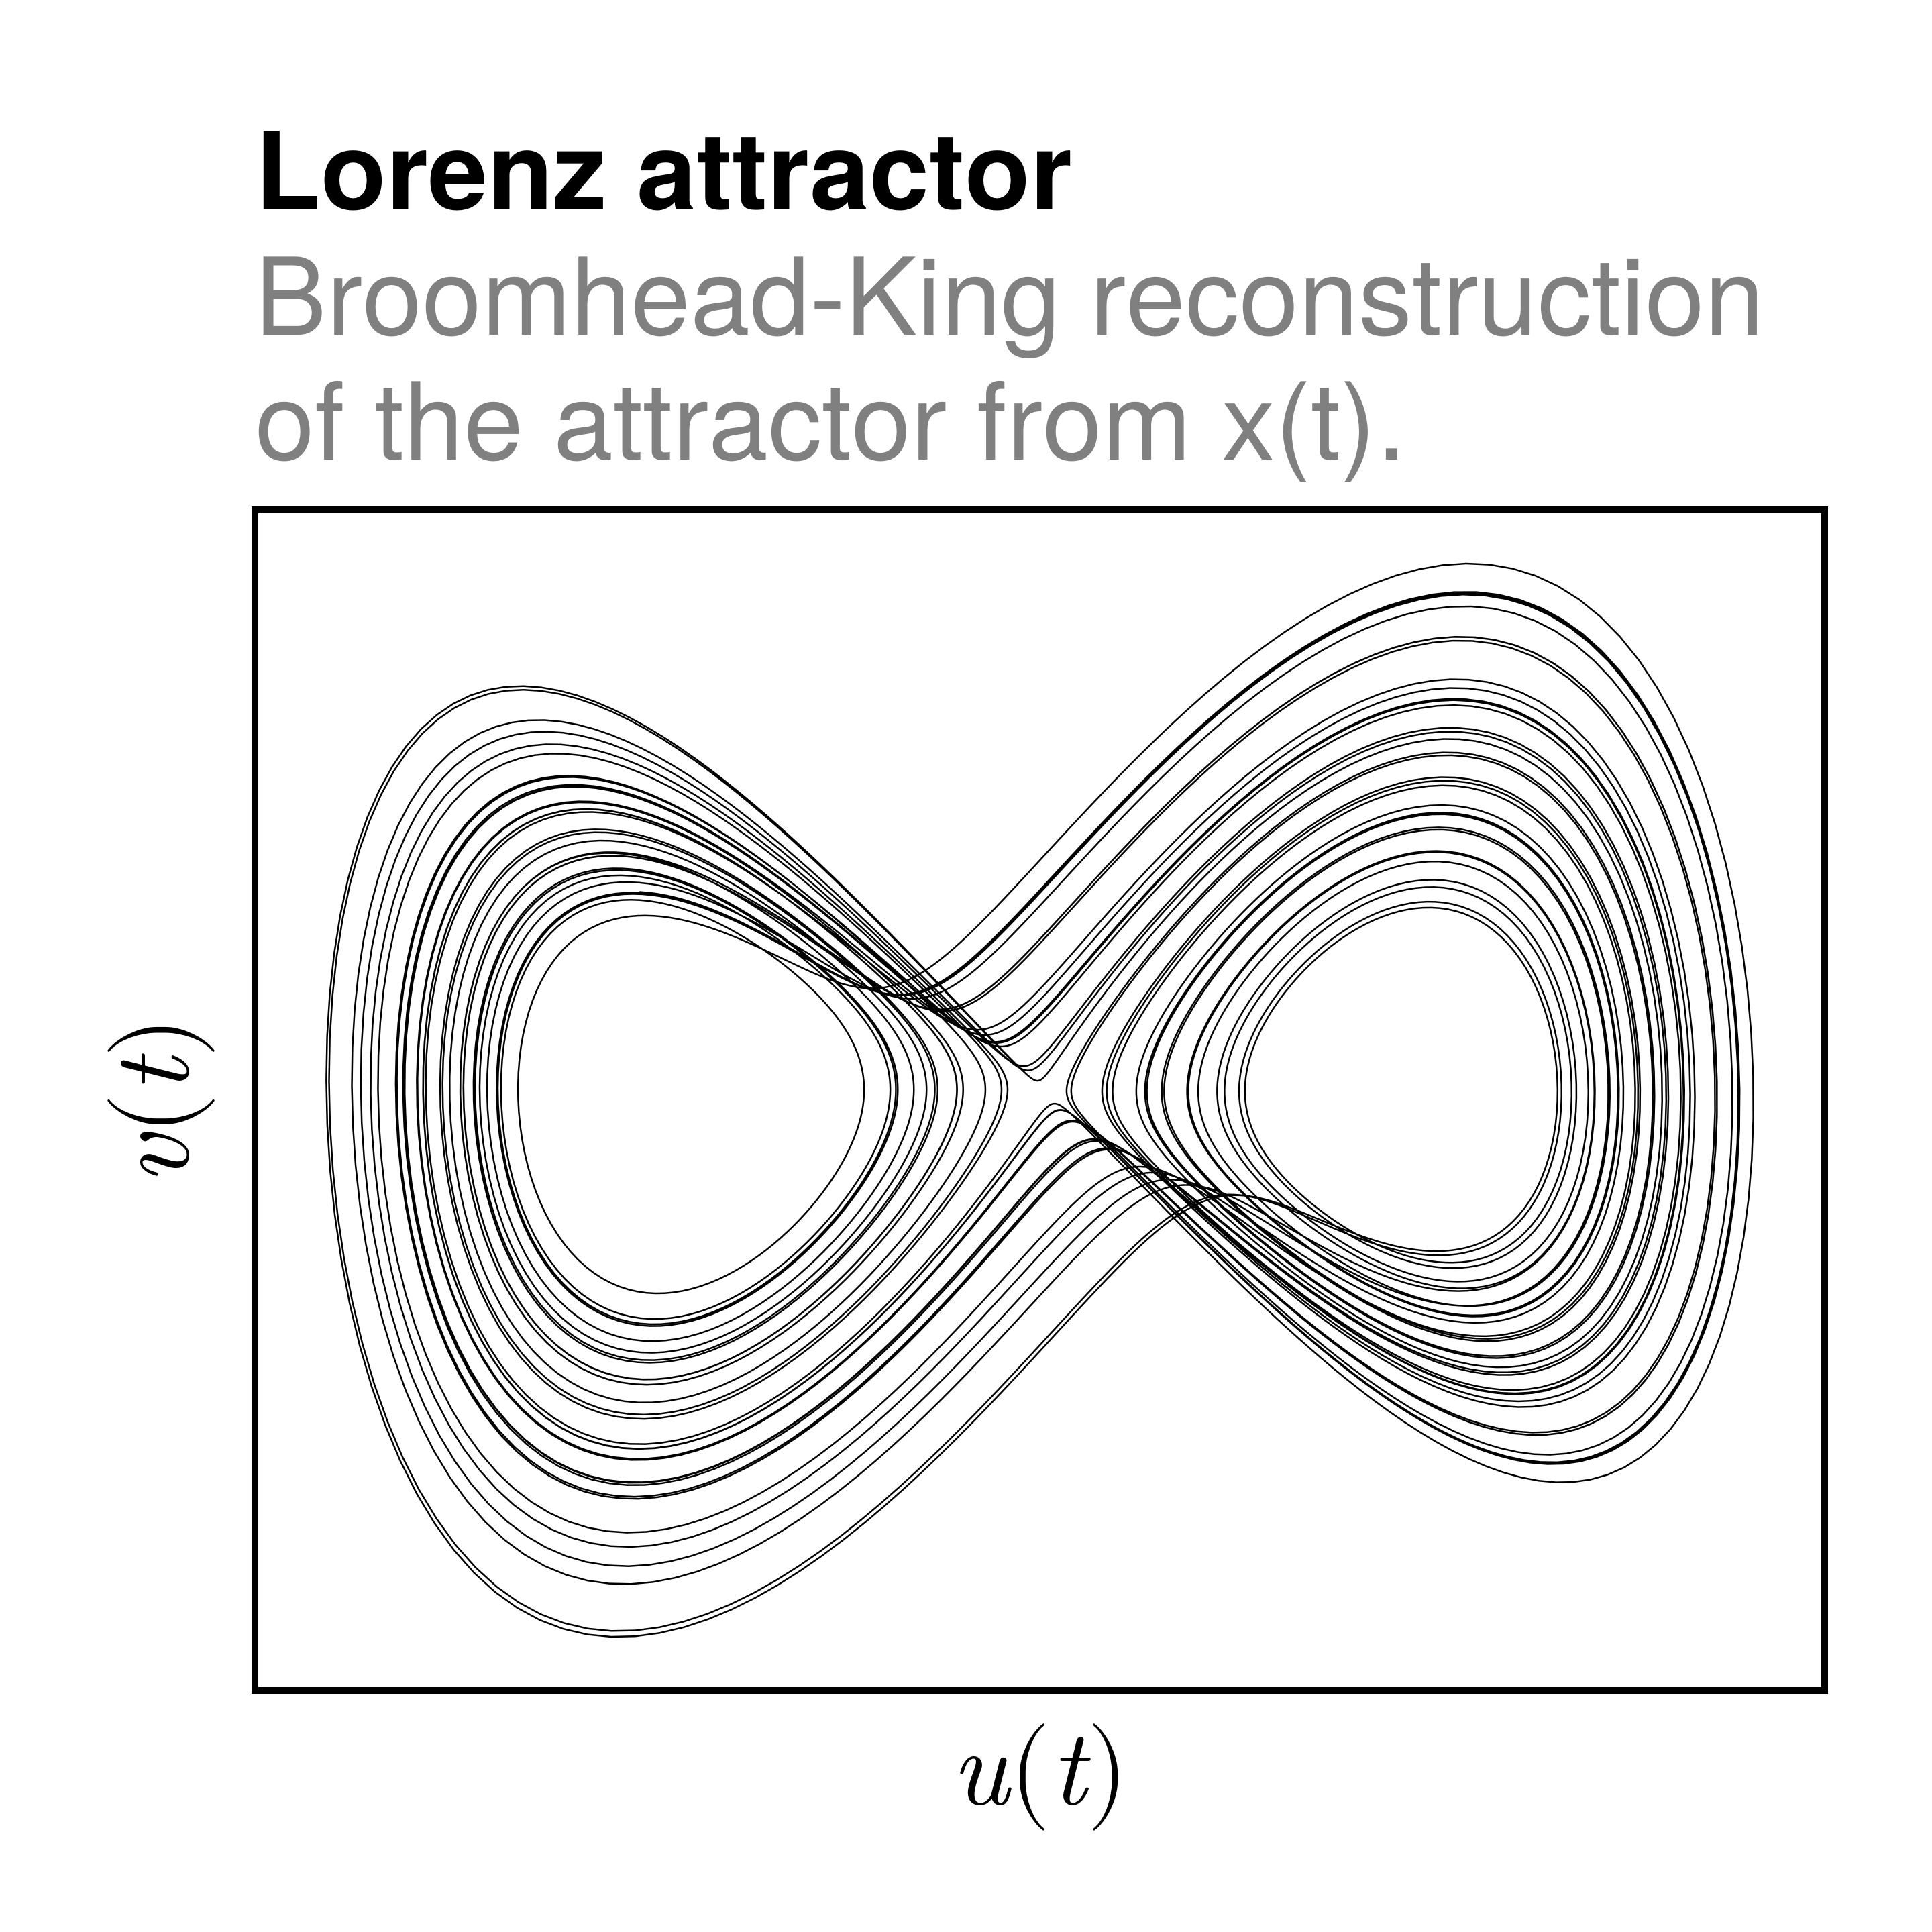
\includegraphics[width=\textwidth]{Lorenz_attractor_reconstruction}
    \end{minipage}
    \vfill
  \end{frame}

  \begin{frame}
    \vfill
    \begin{minipage}{.48\textwidth}
      Given the reconstructed attractor, use
      %
      \[
        \chi = \rowvec{u, v, w, u^2, uv, uw, v^2, \cdots}
      \]
      %
      to approximate the Koopman singular functions.
    \end{minipage}%
    \hfill
    \begin{minipage}{.48\textwidth}
      \centering
      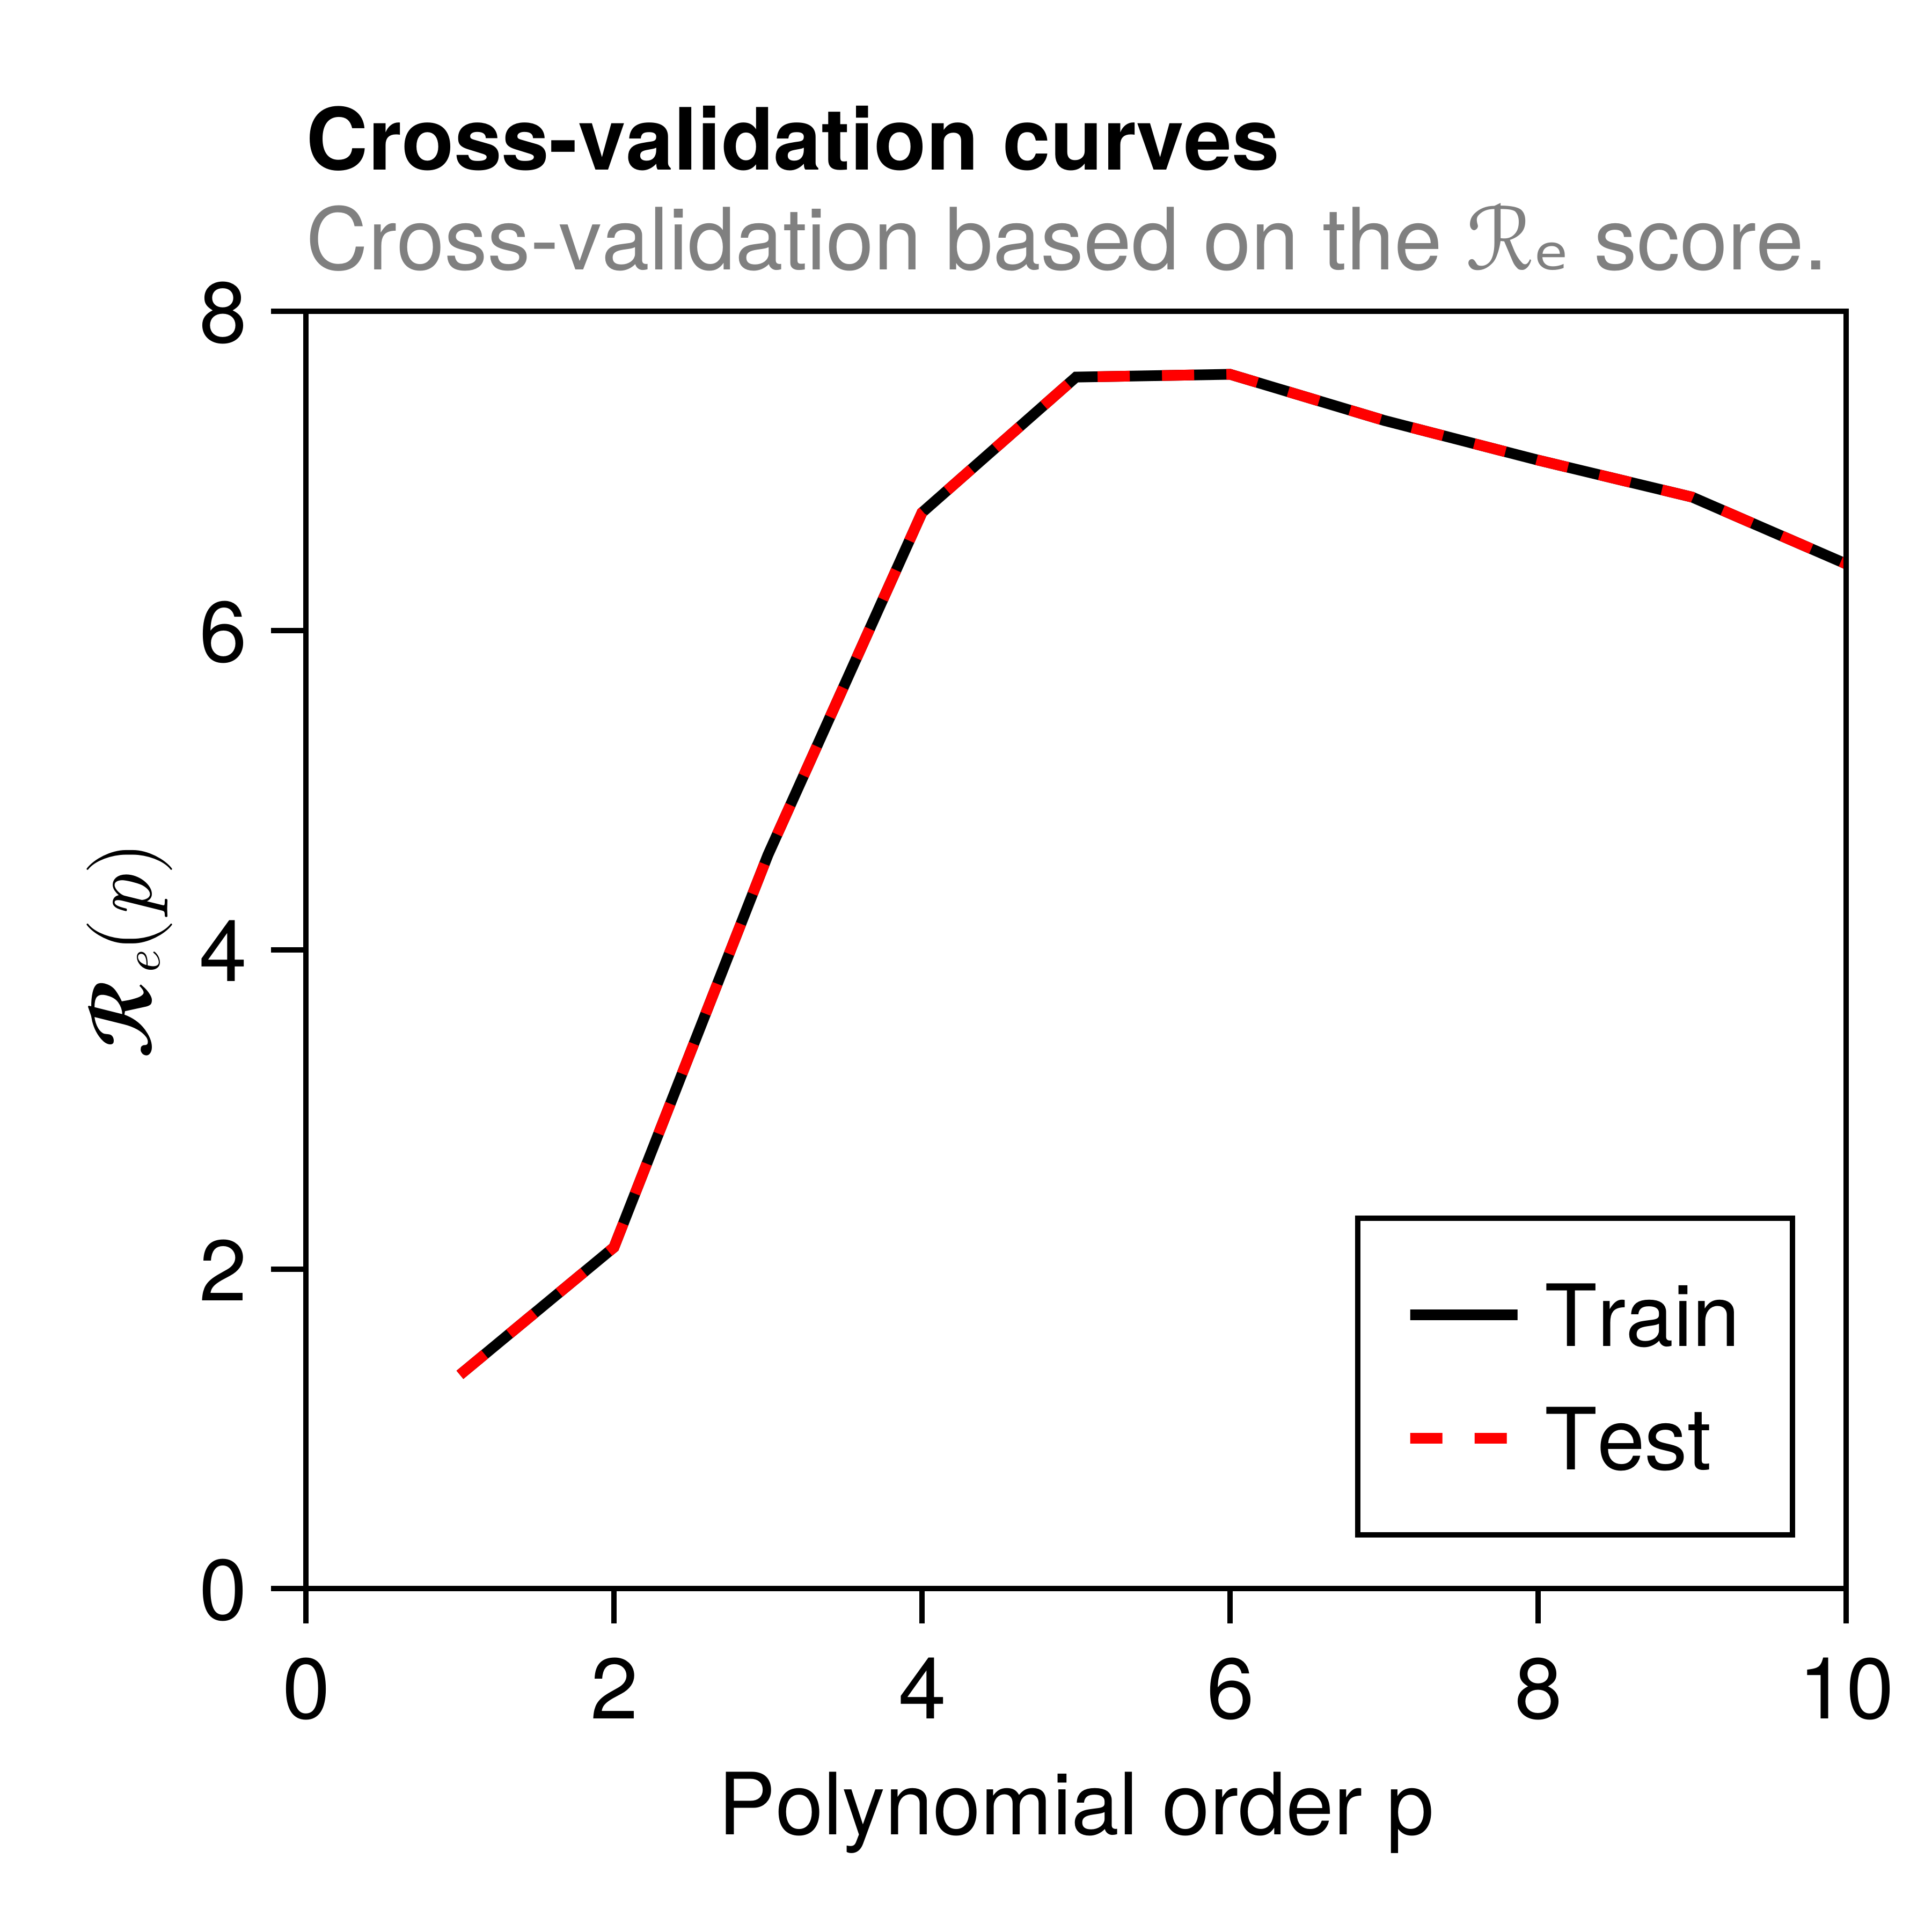
\includegraphics[width=\textwidth]{Lorenz_cross_validation_broomhead}
    \end{minipage}
    \vfill
  \end{frame}

  \begin{frame}
    \vfill
    \centering
    \begin{center}
      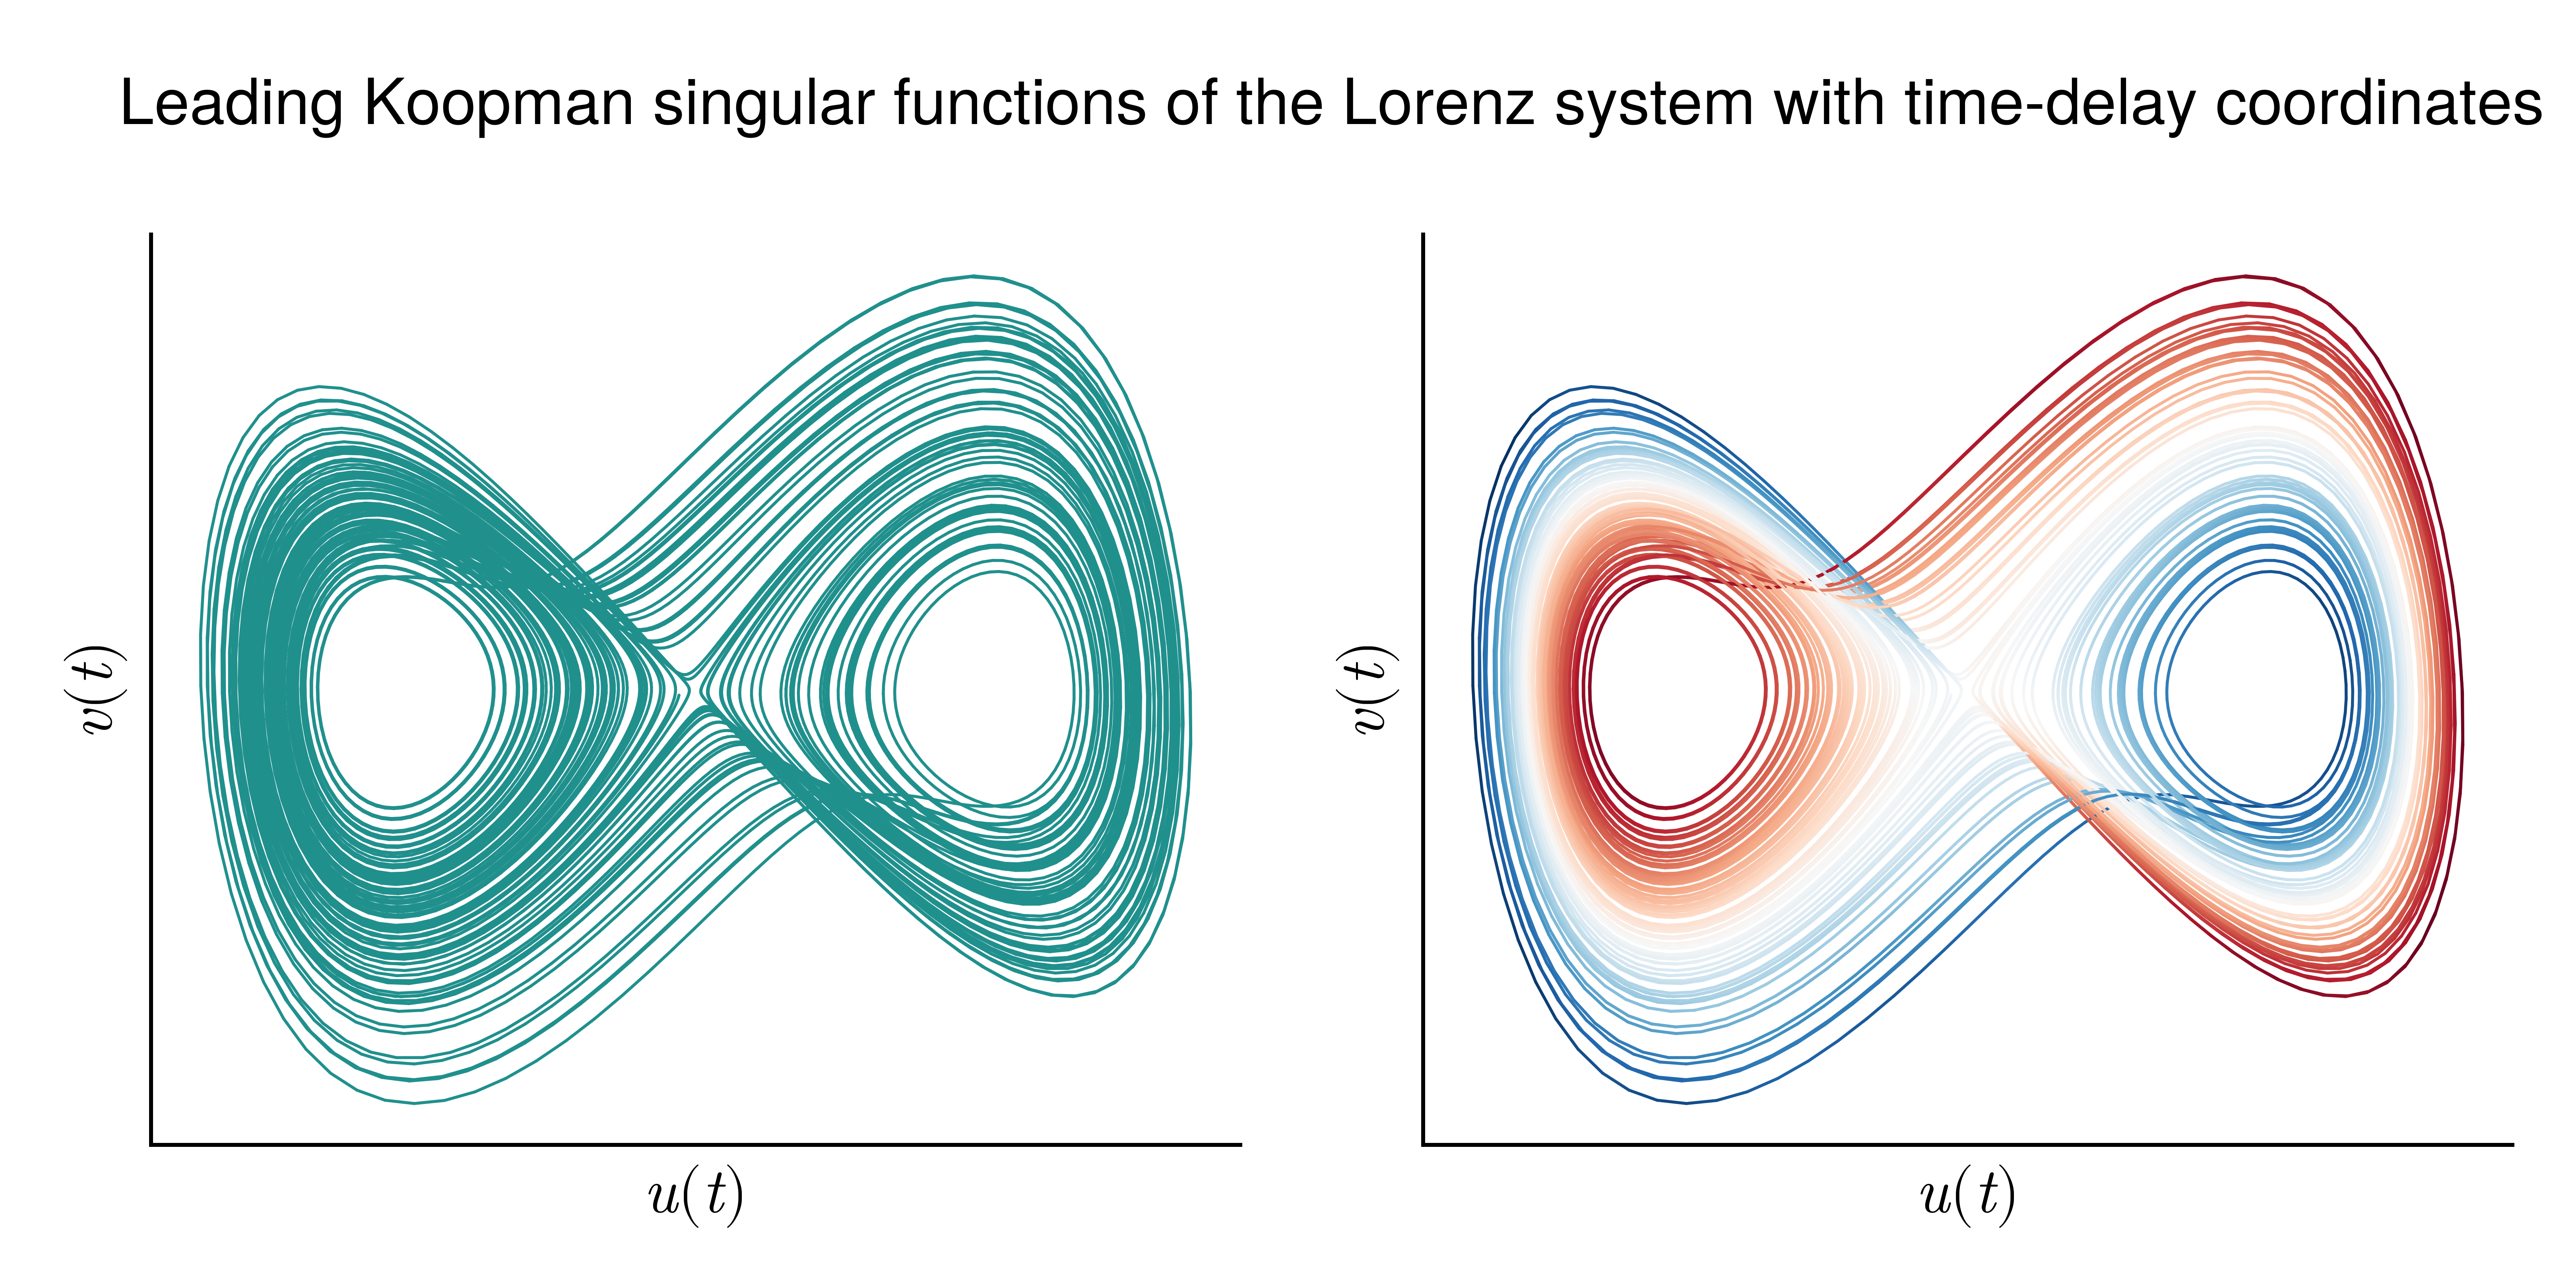
\includegraphics[width=.8\textwidth]{Lorenz_eigenfunctions_broomhead}
    \end{center}
    \vfill
  \end{frame}

  \begin{frame}
    \vfill
    \centering
    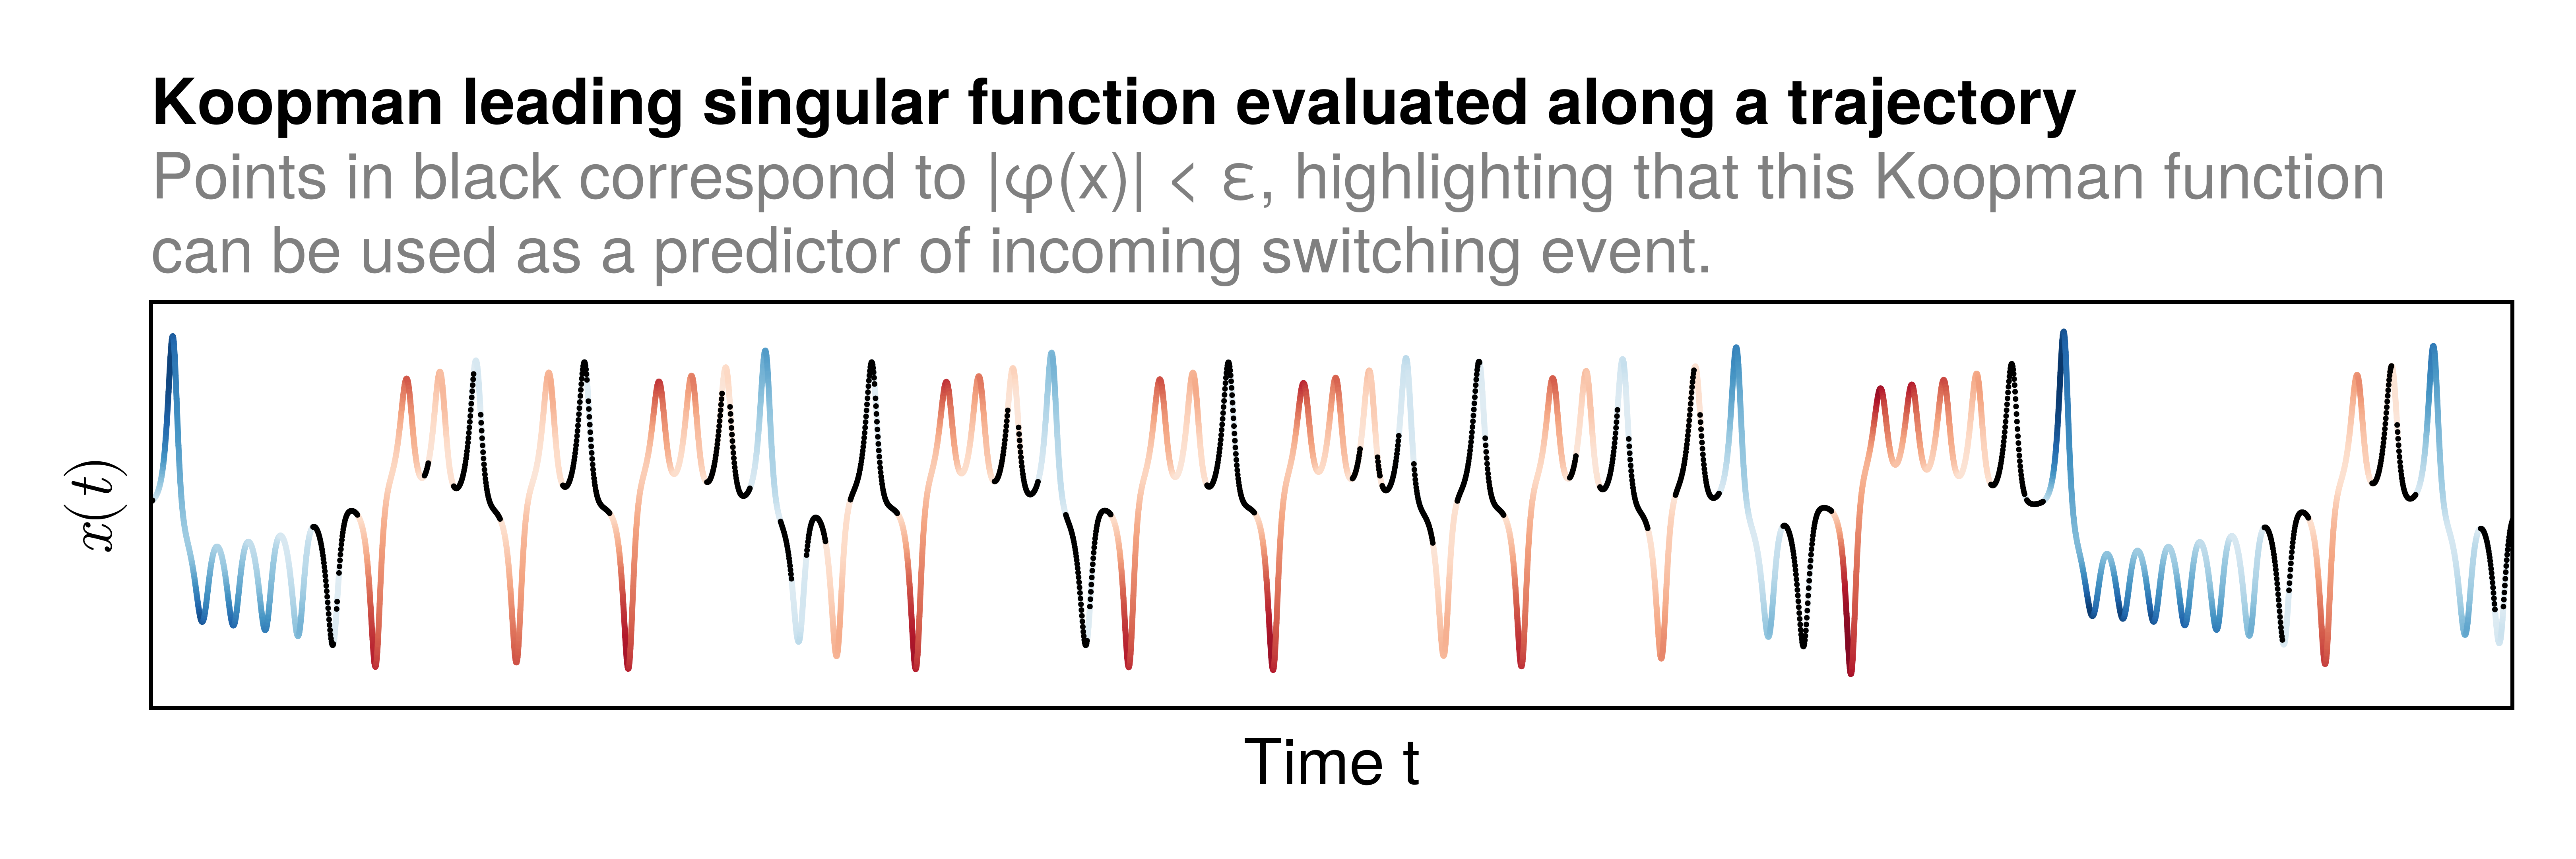
\includegraphics[width=\textwidth]{Lorenz_switch_prediction}
    \vfill
  \end{frame}

  \begin{frame}
    \vfill
    \begin{minipage}{.4\textwidth}
      \centering
      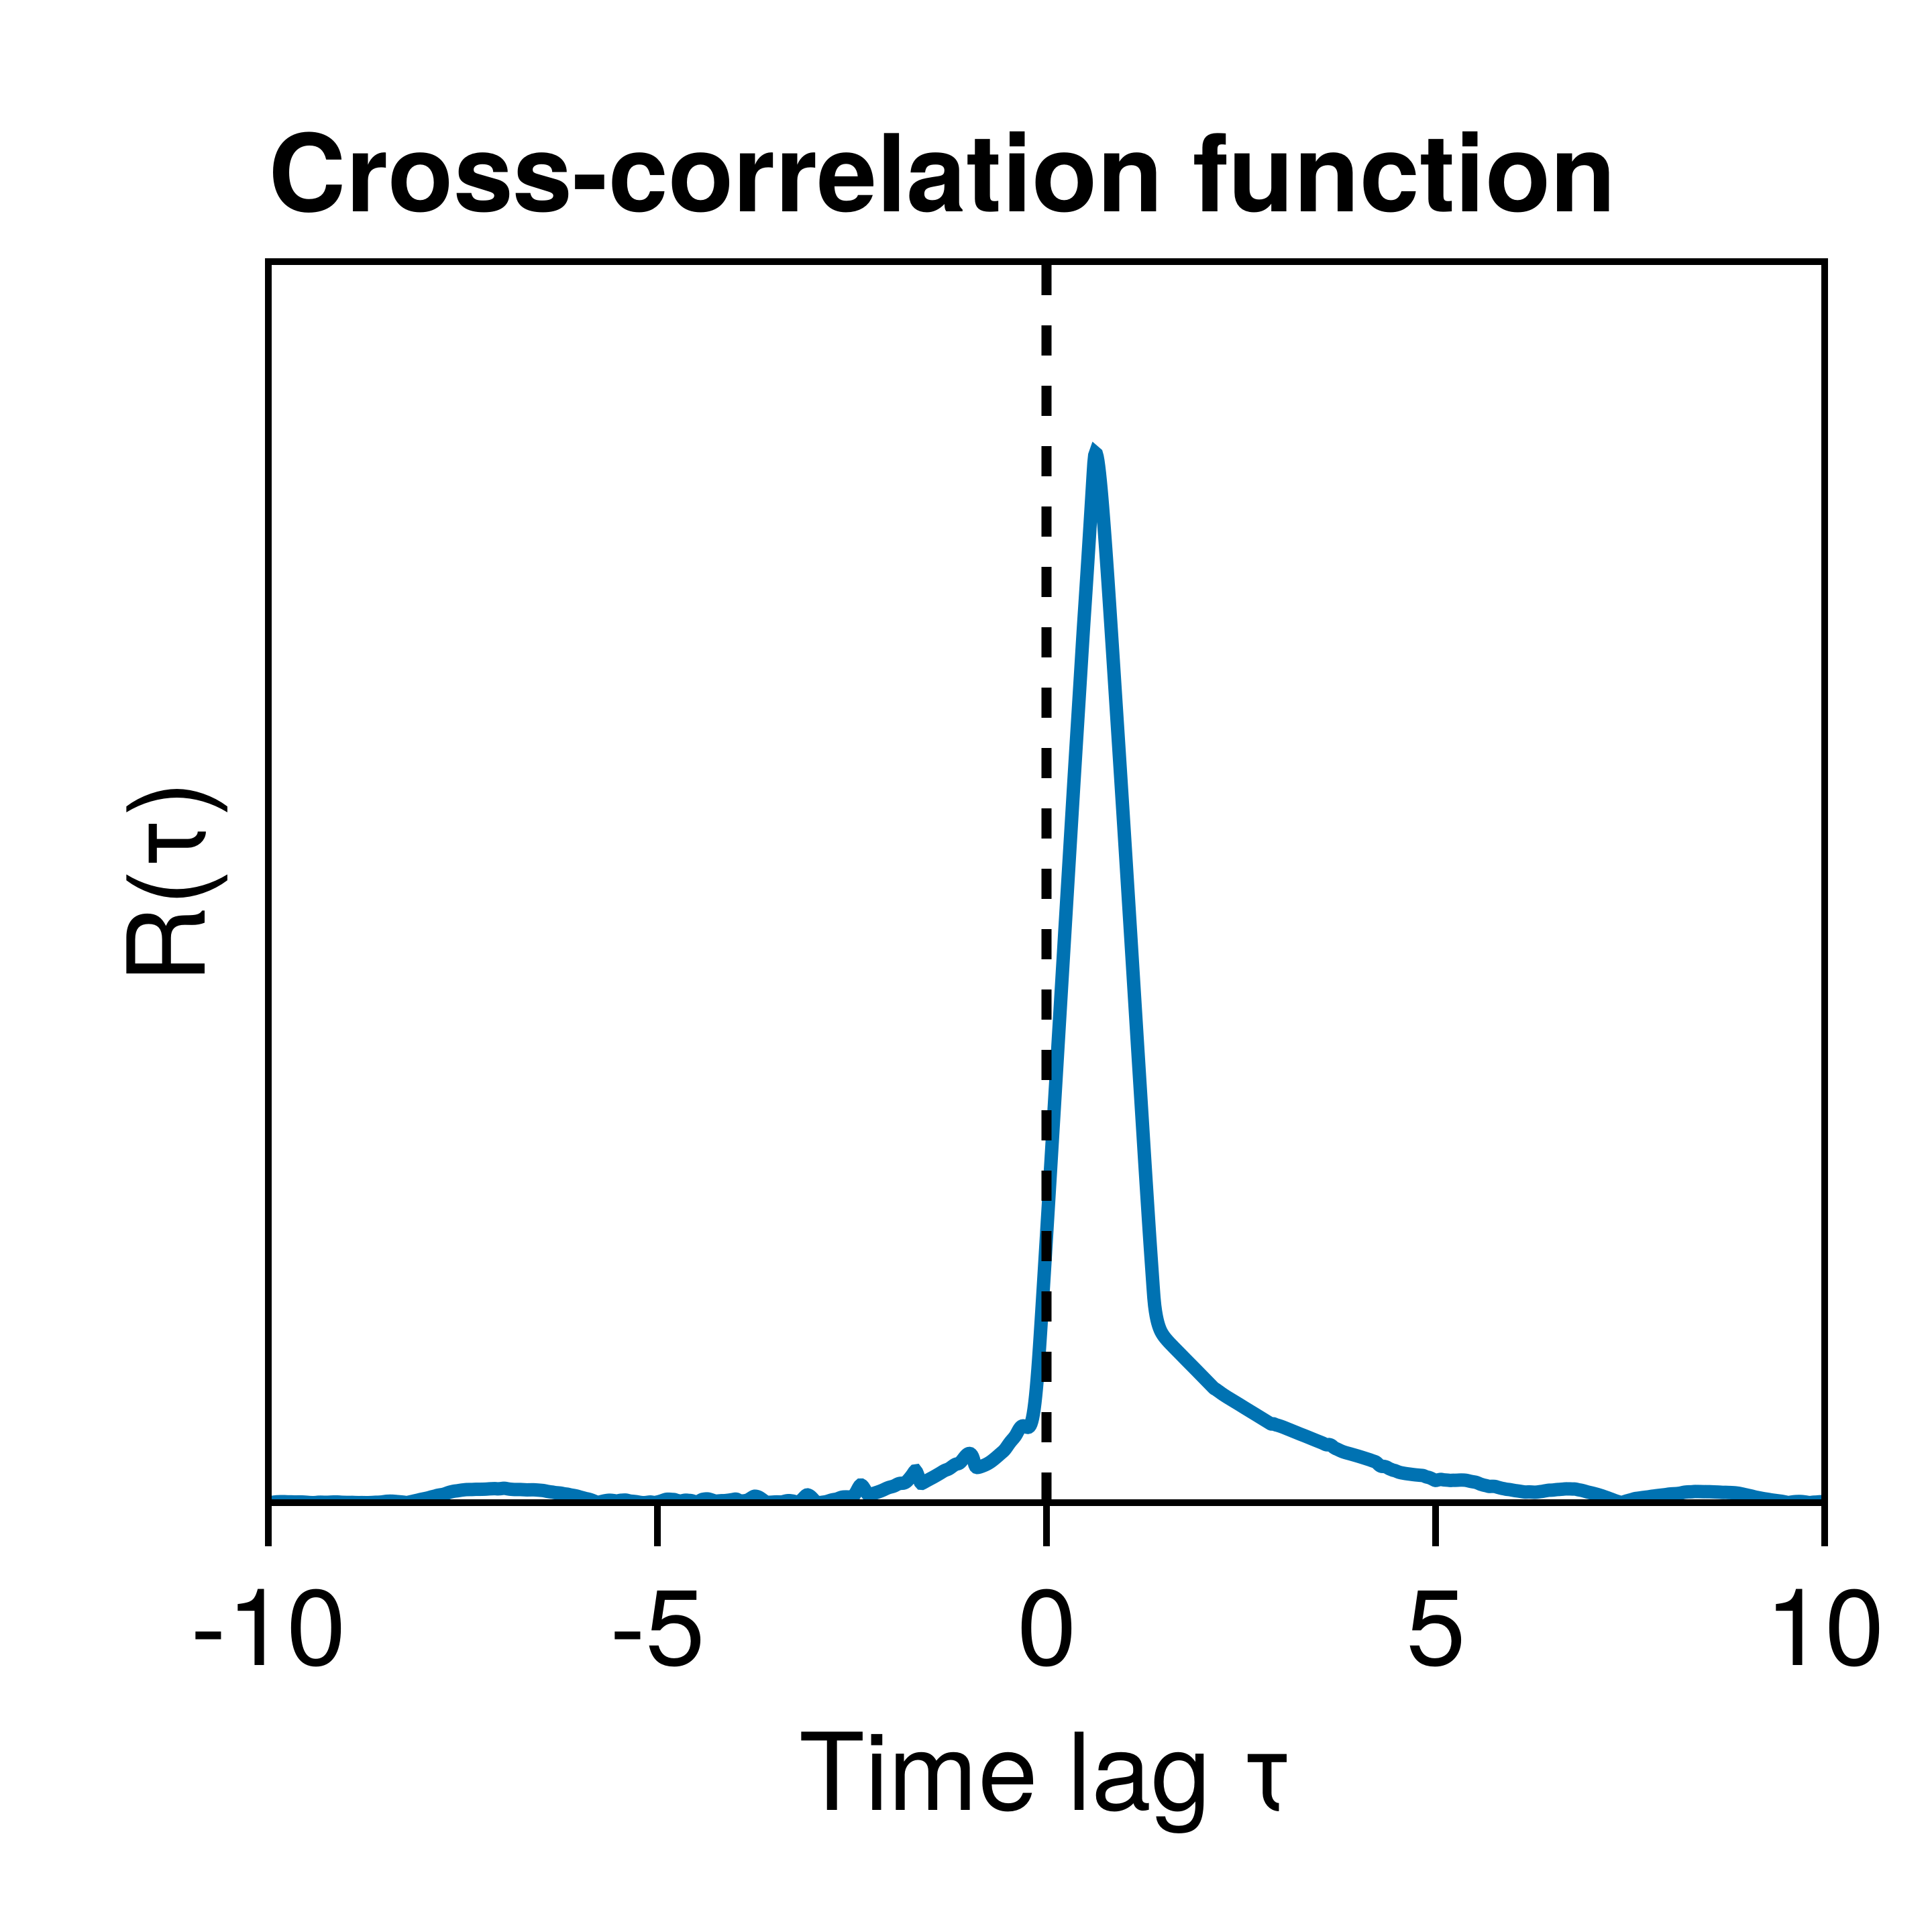
\includegraphics[width=\textwidth]{Lorenz_cross_correlation_prediction}
    \end{minipage}%
    \hfill
    \begin{minipage}{.56\textwidth}
      Let $f(t) = \mathrm{sign}(x_t)$ and $g(t) = \mathrm{sign}(\varphi_1(x_t))$.
      On average, $g(t)$ predicts a switching event \textbf{a whole period} before it occurs.
    \end{minipage}
    \vfill
  \end{frame}

}


\begin{frame}
  \vfill

  \begin{minipage}{.60\textwidth}
    \vfill
    \centering

    \vfill
  \end{minipage}%
  \hfill
  \begin{minipage}{.36\textwidth}
    {\Large
      \textbf{
        \begin{flushright}
          Application to a flow example
        \end{flushright}
      }
    }
  \end{minipage}
  
  \vfill
\end{frame}

\begin{frame}
  \vfill
  \begin{minipage}{.28\textwidth}
    \centering
    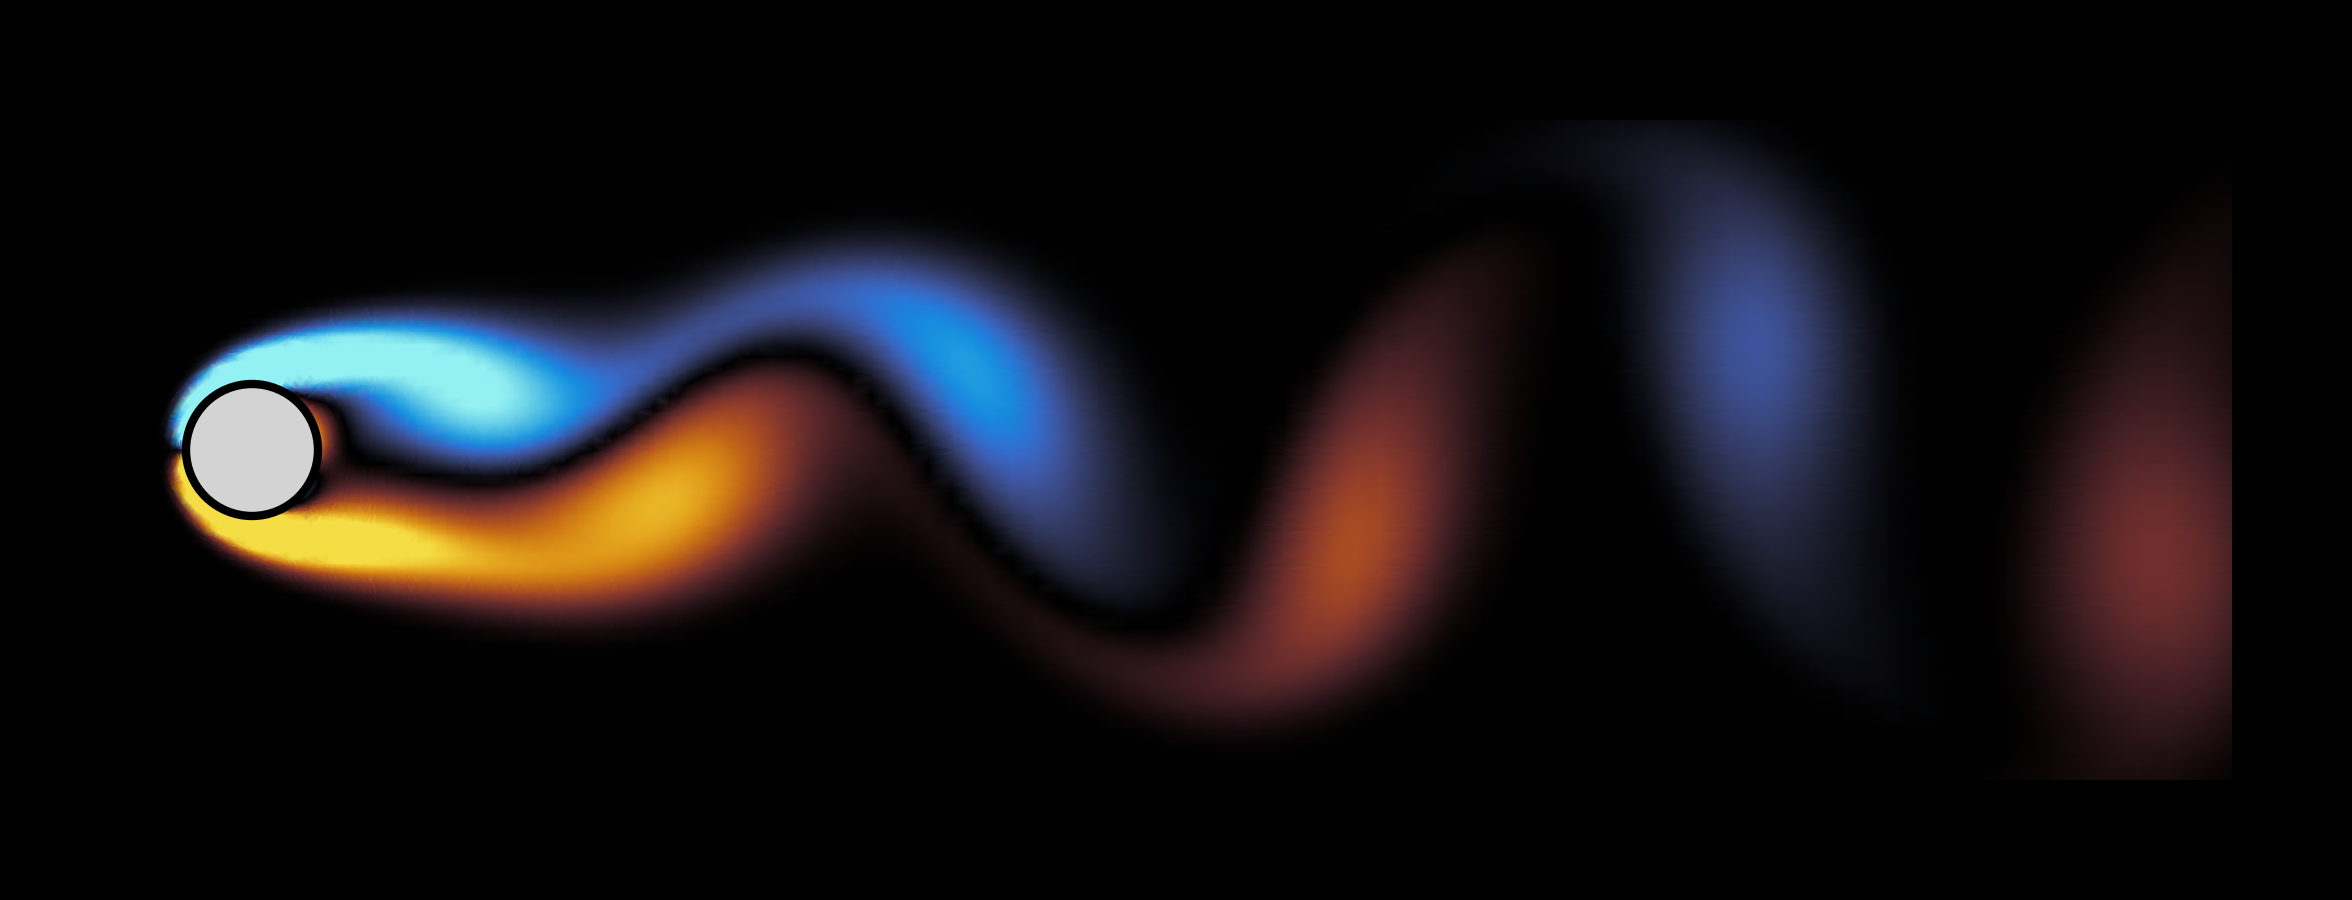
\includegraphics[height=.4\textheight, angle=-90, origin=c]{von_karman}
  \end{minipage}%
  \hfill
  \begin{minipage}{.68\textwidth}
    \textbf{Low-Re cylinder flow :} Canonical fluid example of a self-sustained weakly nonlinear oscillator.

    \bigskip

    In the rest, we'll assume that we only have access to the instantaneous lift and drag coefficients.
  \end{minipage}
  \vfill
\end{frame}

\begin{frame}
  \vfill
  \begin{minipage}{.48\textwidth}
    The dynamics being periodic, the attractor is a simple limit cycle.
  \end{minipage}%
  \hfill
  \begin{minipage}{.48\textwidth}
    \centering
    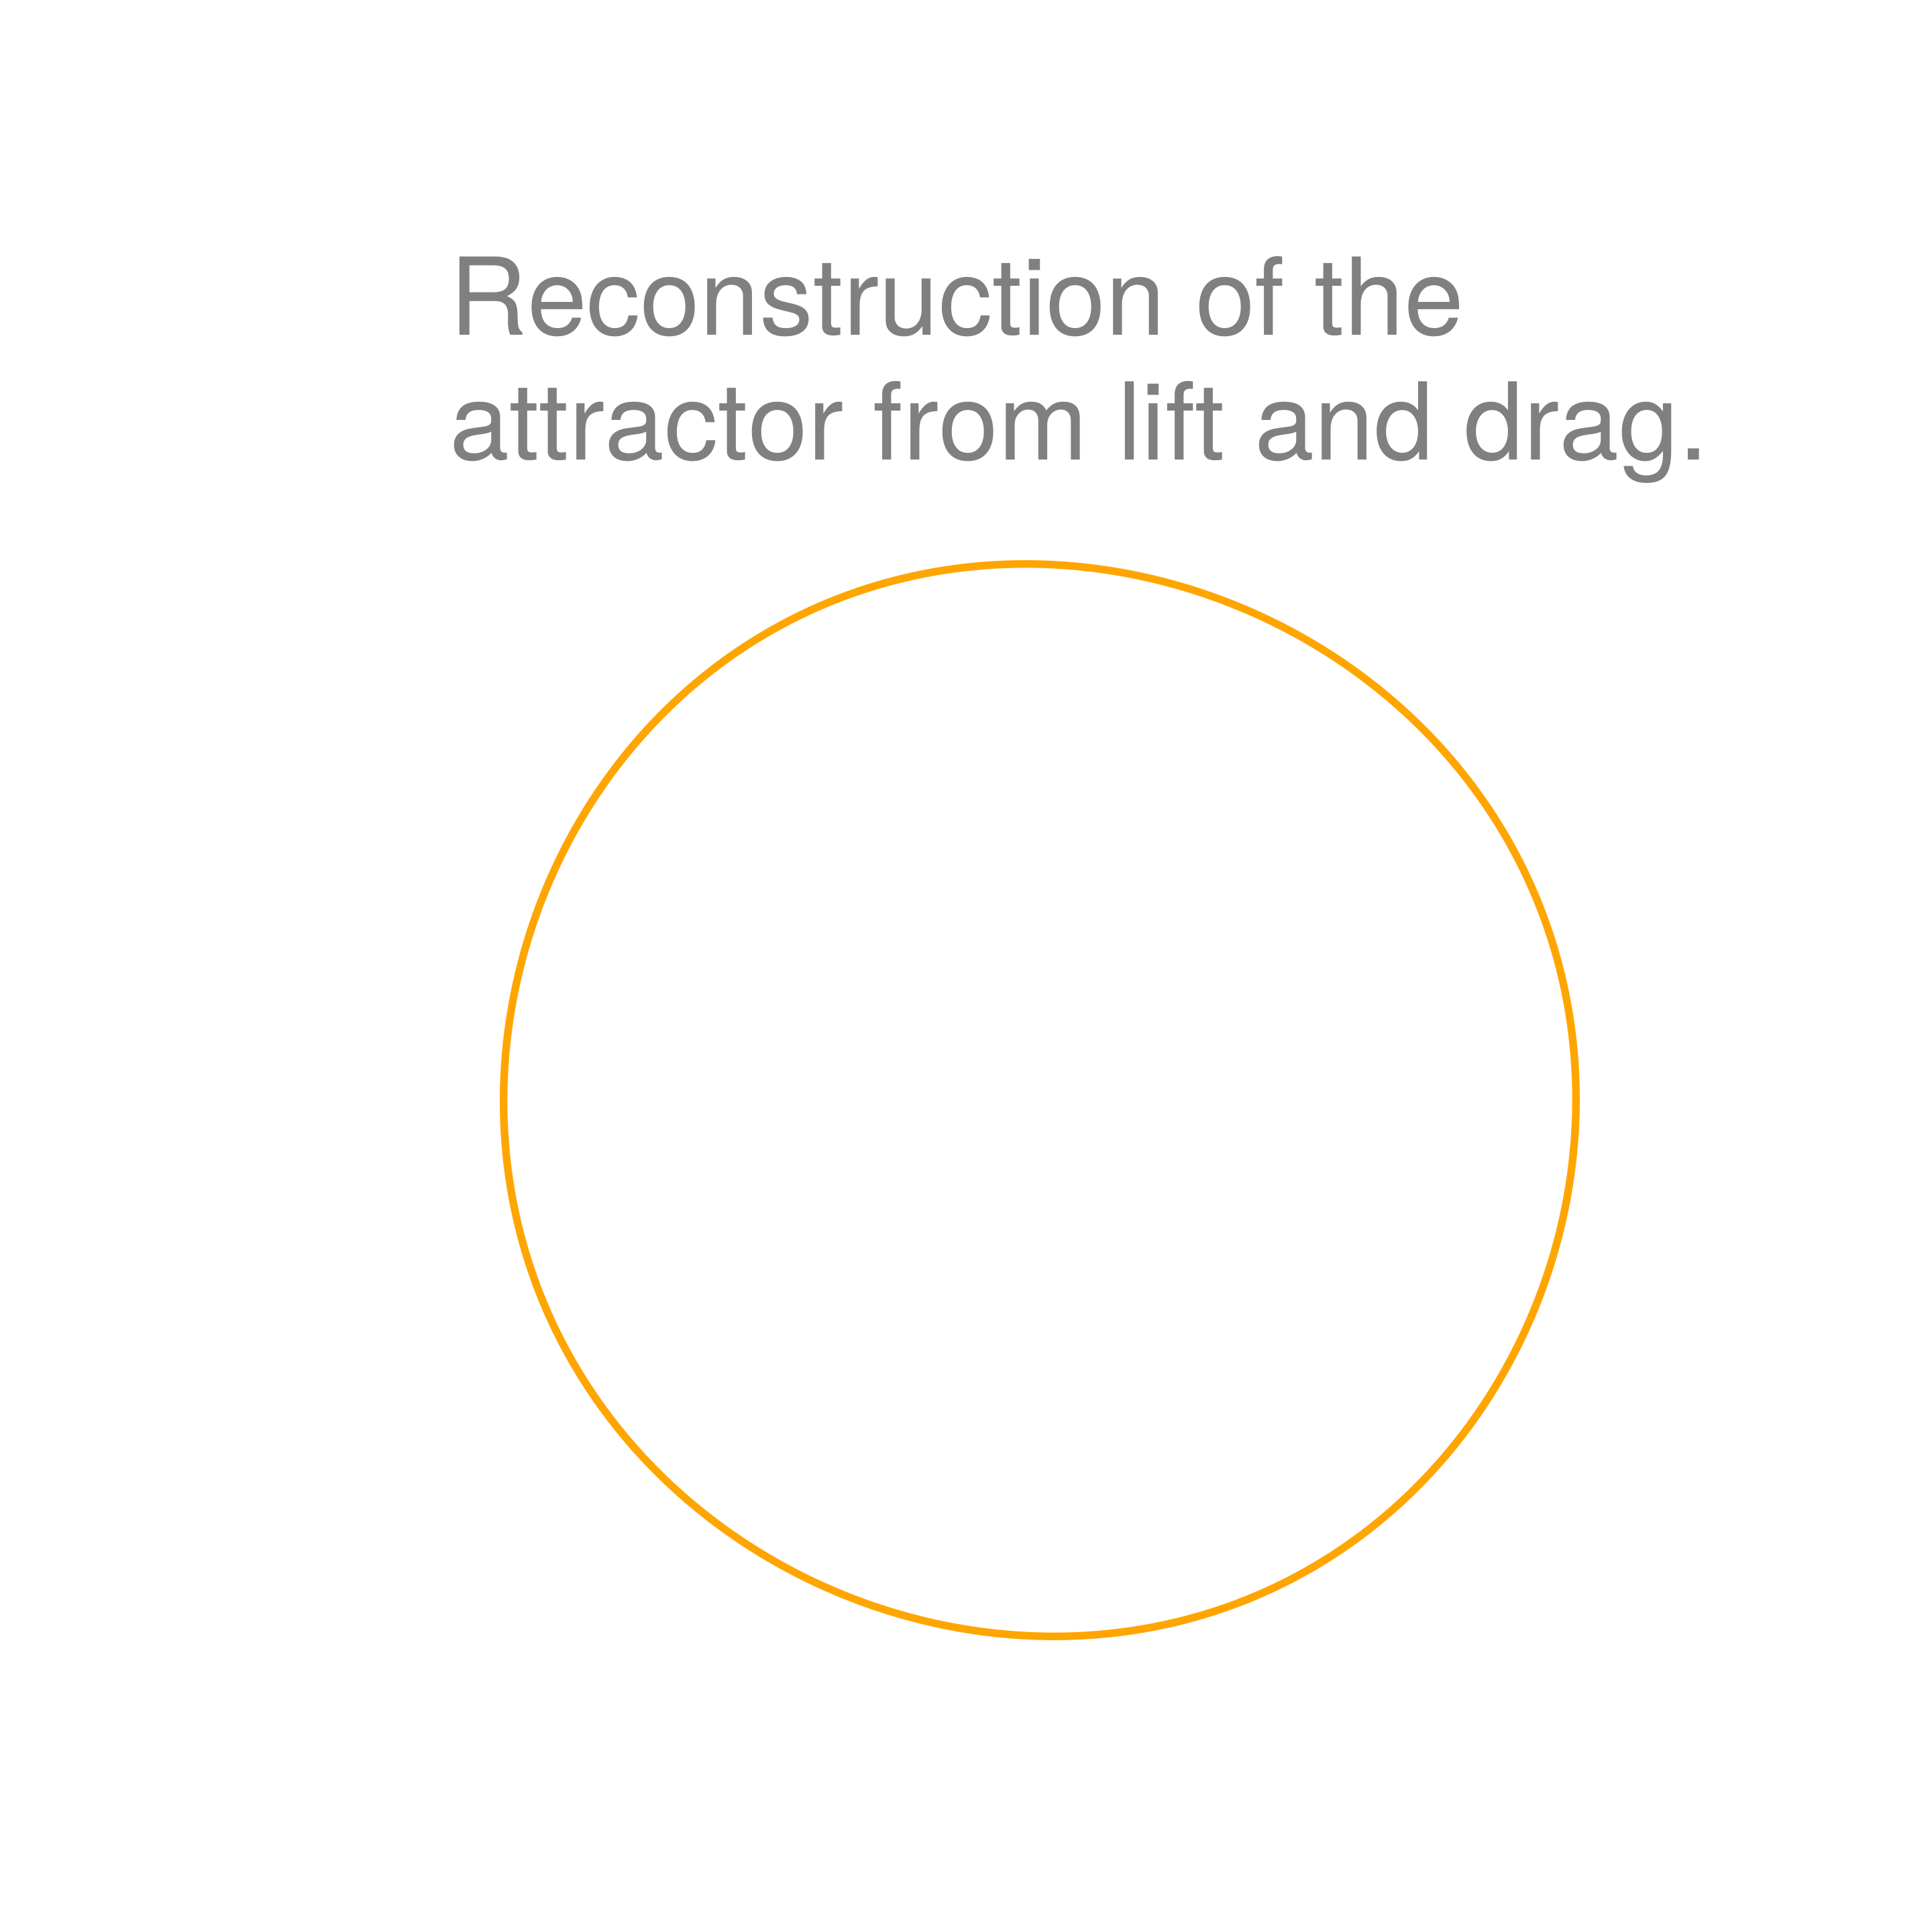
\includegraphics[width=\textwidth]{cylinder_attractor_reconstruction}
  \end{minipage}
  \vfill
\end{frame}

\begin{frame}
  \vfill
  \begin{minipage}{.48\textwidth}
    Given $\vb{U}$, $\vb{K}$, and $\vb{V}$, compute the approximate Koopman eigenvalues
    %
    \[
      \lambda = \mathrm{eig}\left( \vb{K} \vb{V}^T \vb{U} \right)
    \]
    %
    and corresponding residual.
  \end{minipage}%
  \hfill
  \begin{minipage}{.48\textwidth}
    \centering
    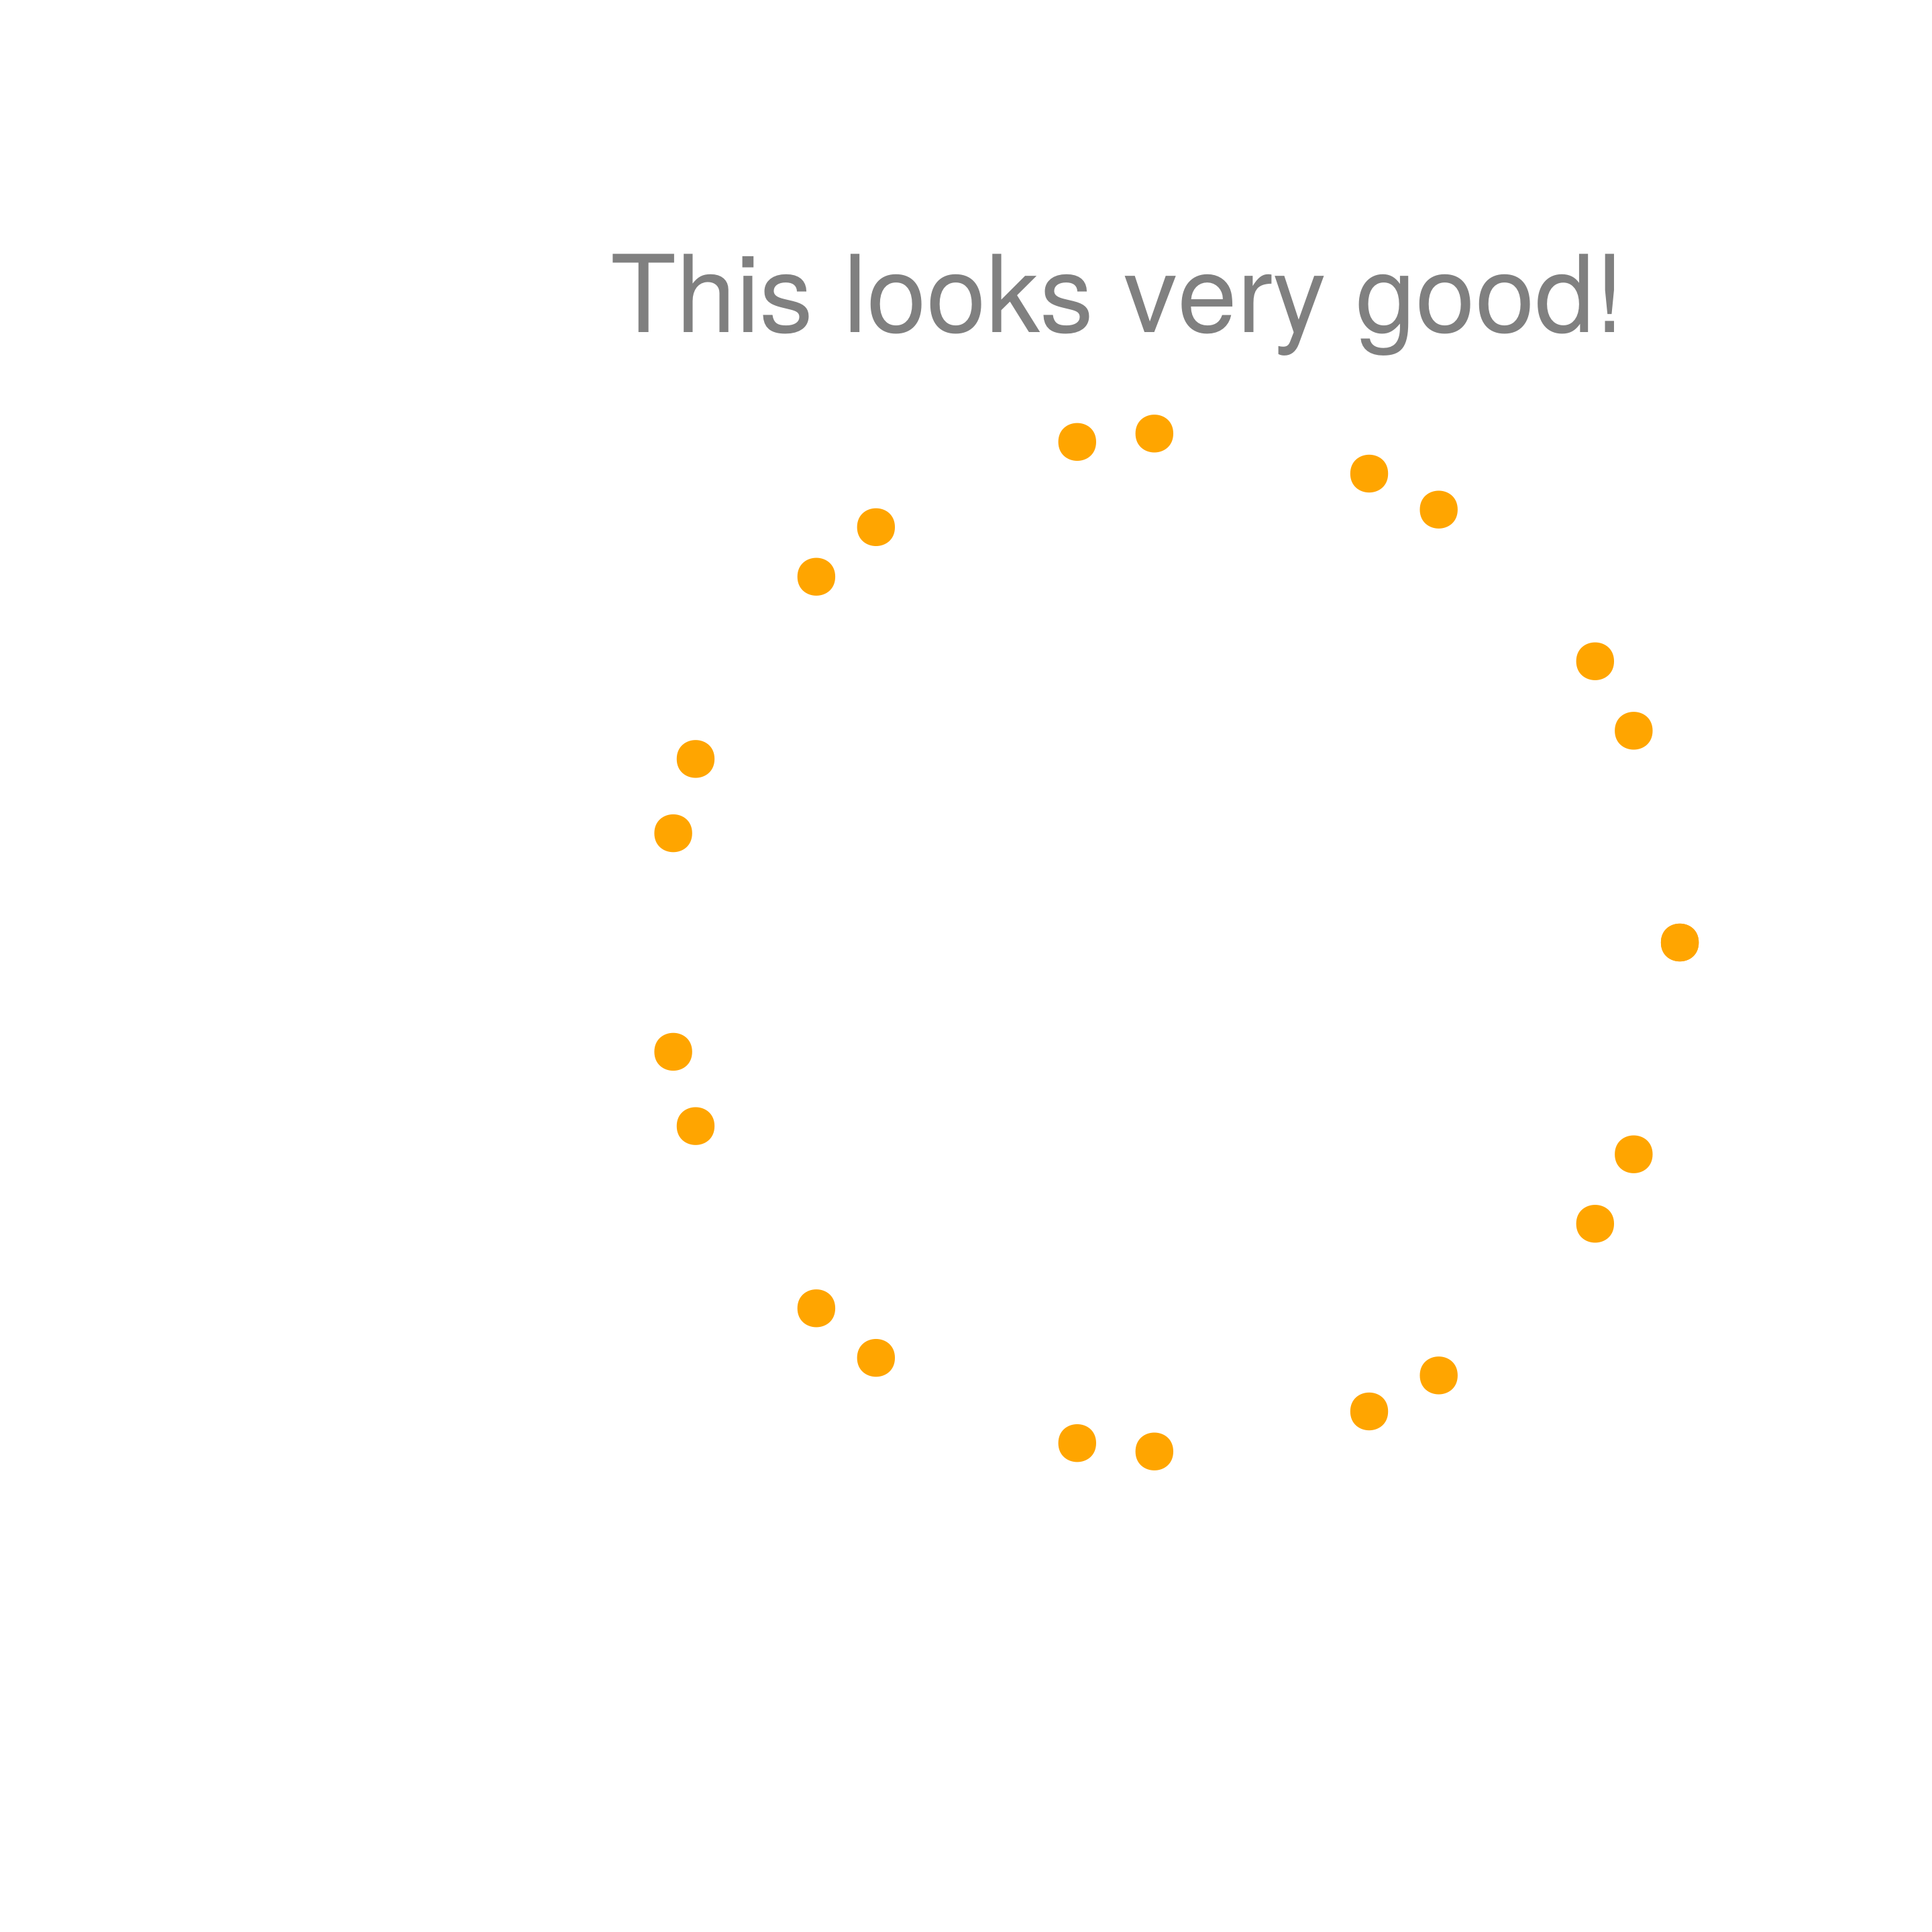
\includegraphics[width=\textwidth]{Cylinder_eigenvalues}
  \end{minipage}

  \vfill
\end{frame}


\begin{frame}
  \vfill
  \begin{minipage}{.48\textwidth}
    Given $\vb{U}$, $\vb{K}$, and $\vb{V}$, compute the approximate Koopman eigenvalues
    % 
    \[
      \lambda = \mathrm{eig}\left( \vb{K} \vb{V}^T \vb{U} \right)
    \]
    % 
    and corresponding residual.
  \end{minipage}%
  \hfill
  \begin{minipage}{.48\textwidth}
    \centering
    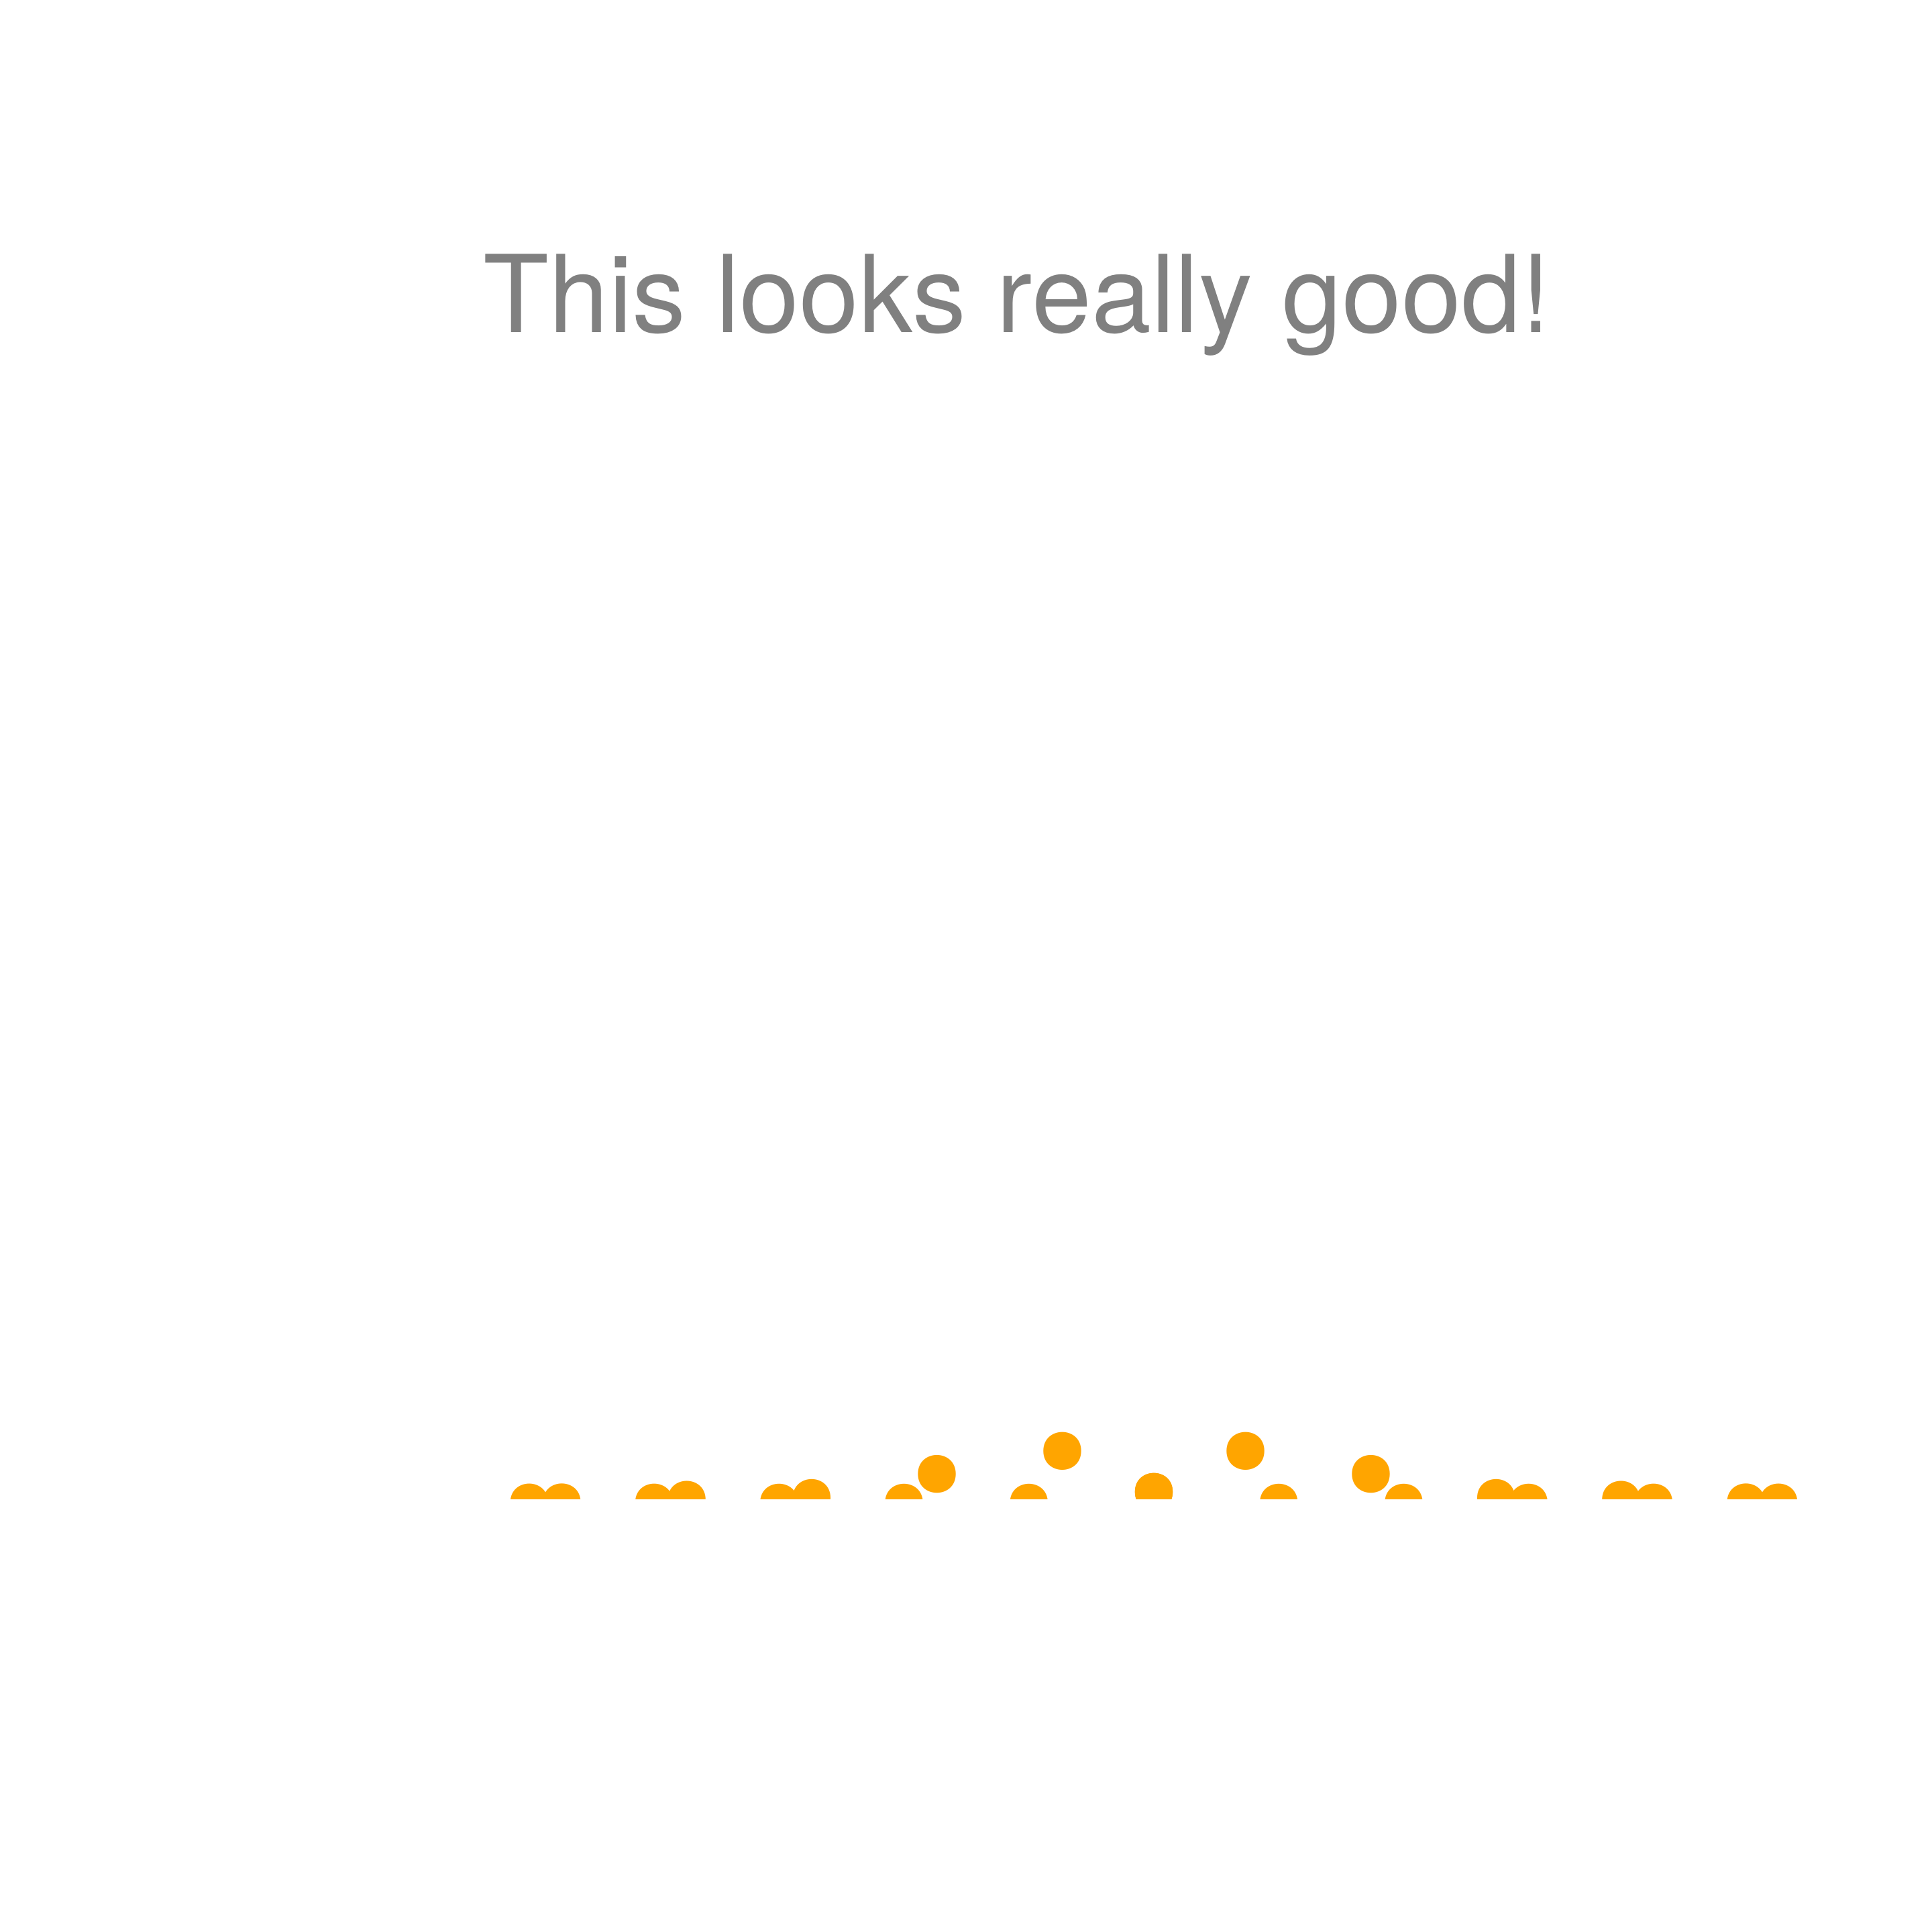
\includegraphics[width=\textwidth]{Cylinder_eigenvalues_residual}
  \end{minipage}

  \vfill
\end{frame}

\begin{frame}
  \vfill
  \centering
  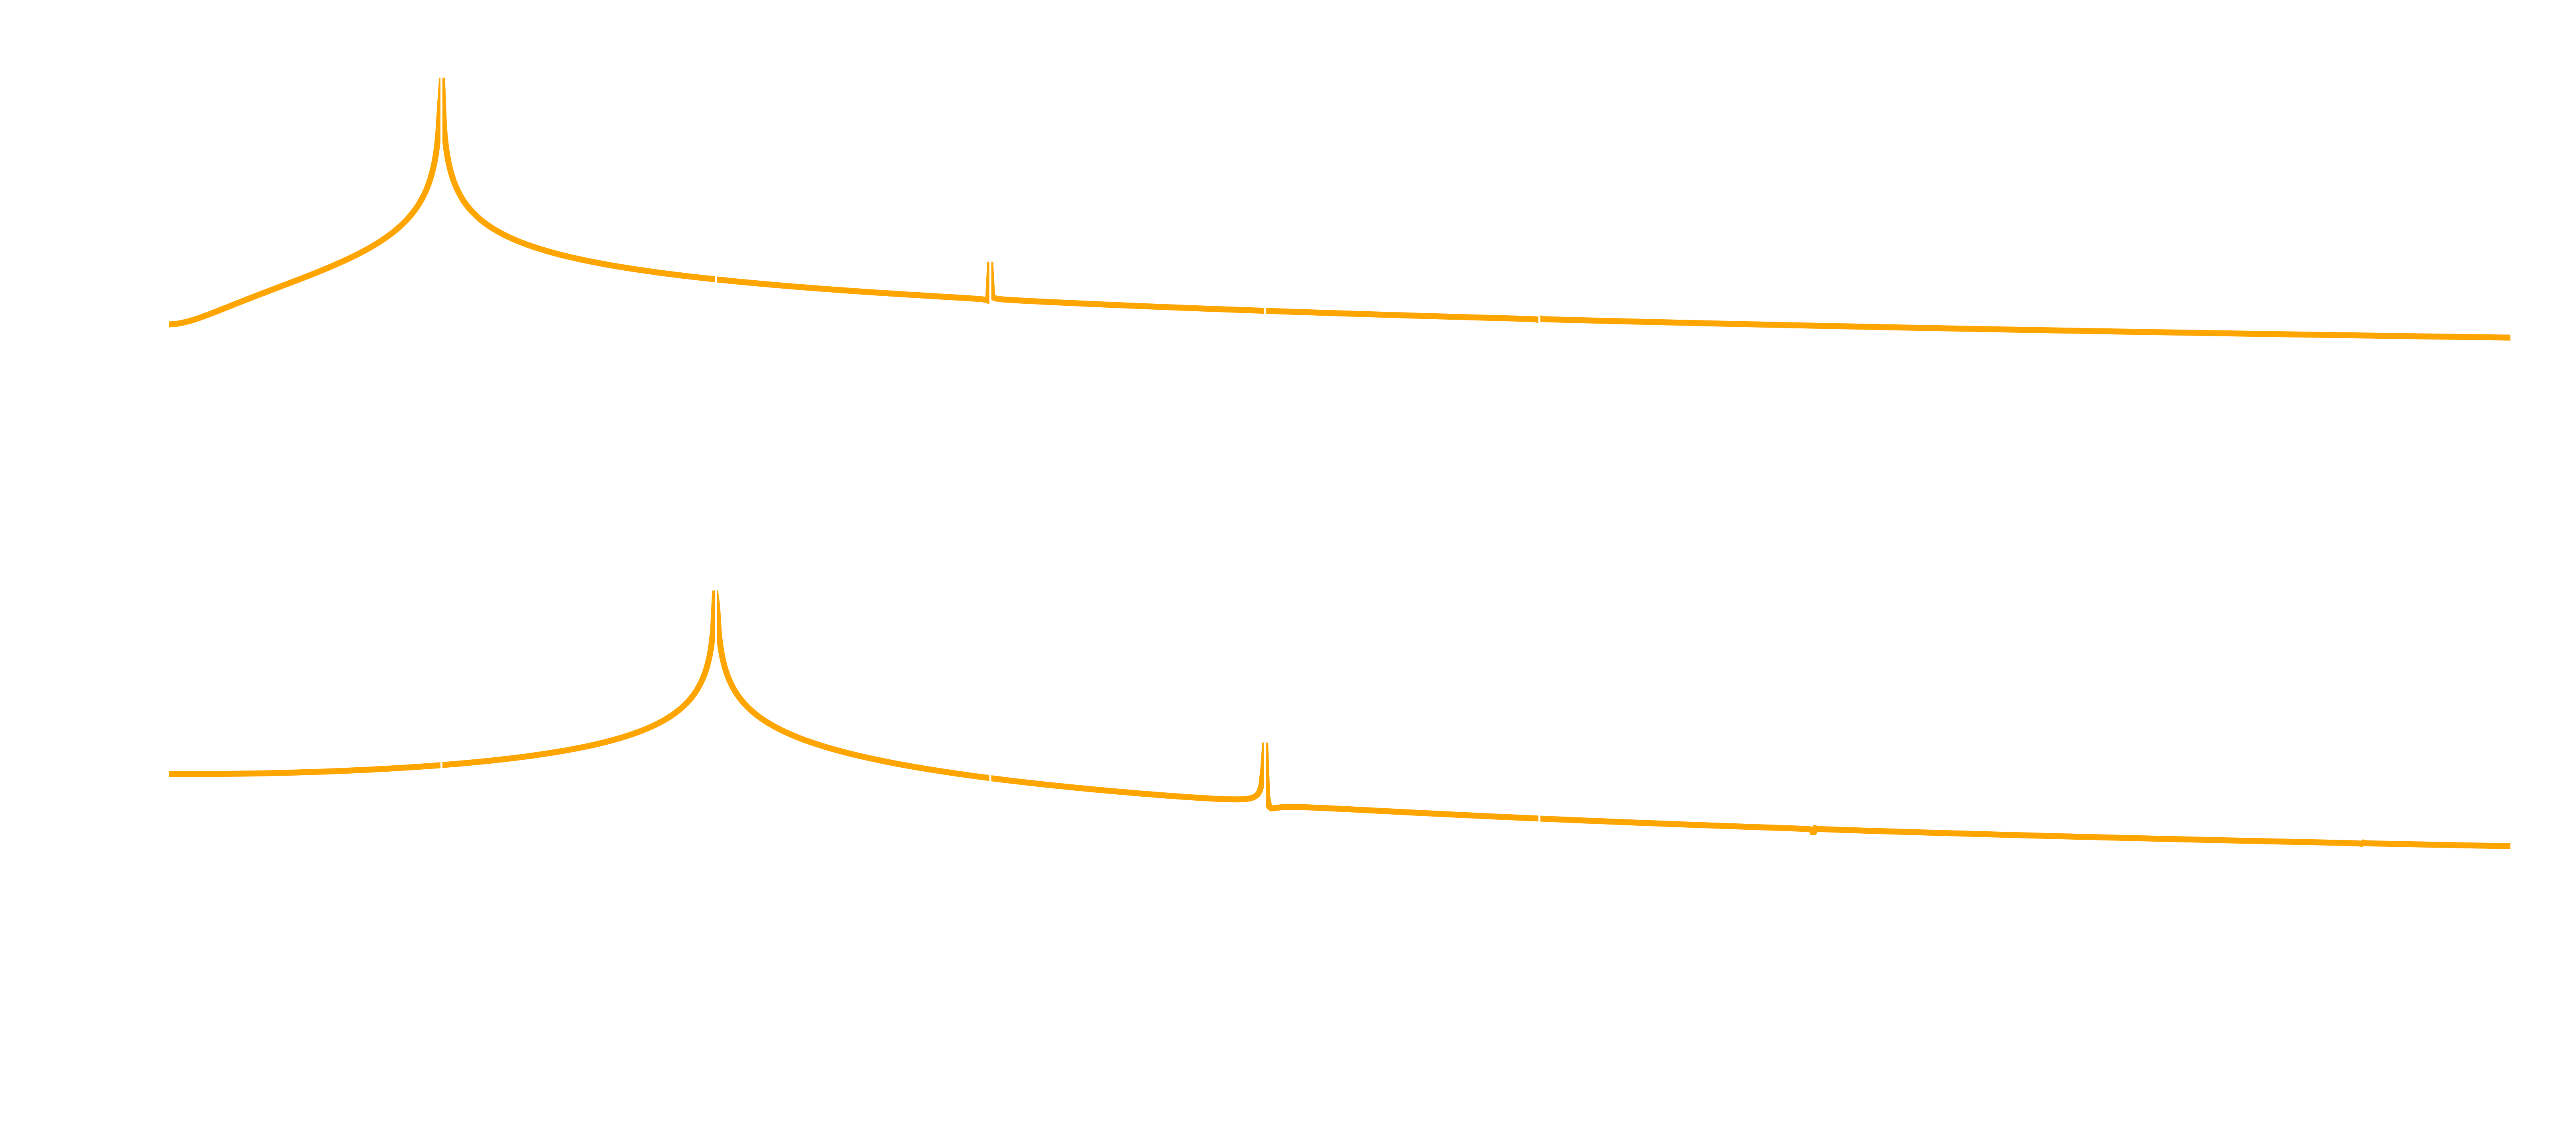
\includegraphics[width=\textwidth]{Cylinder_fft}
  \vfill
\end{frame}

\begin{frame}
  \vfill
  \begin{minipage}{.68\textwidth}
    \textbf{Shear-driven cavity flow :} Canonical fluid example for reduced-order modelling and flow control.

    \bigskip

    In the rest, we'll assume that we only have access to the fluctuation's kinetic energy.
  \end{minipage}%
  \hfill
  \begin{minipage}{.28\textwidth}
    \centering
  \end{minipage}%
  
  \vfill
\end{frame}

\begin{frame}
  \vfill
  \begin{minipage}{.48\textwidth}
    The dynamics being quasi-periodic, the attractor is a $T_2$-torus.
  \end{minipage}%
  \hfill
  \begin{minipage}{.48\textwidth}
    \centering
  \end{minipage}
  \vfill
\end{frame}

\begin{frame}
  \vfill
  \begin{minipage}{.48\textwidth}
    Given $\vb{U}$, $\vb{K}$, and $\vb{V}$, compute the approximate Koopman eigenvalues
    %
    \[
      \lambda = \mathrm{eig}\left( \vb{K} \vb{V}^T \vb{U} \right)
    \]
    %
    and corresponding residual.
  \end{minipage}%
  \hfill
  \begin{minipage}{.48\textwidth}
    \centering
  \end{minipage}

  \vfill
\end{frame}


\begin{frame}
  \vfill
  \begin{minipage}{.48\textwidth}
    Given $\vb{U}$, $\vb{K}$, and $\vb{V}$, compute the approximate Koopman eigenvalues
    % 
    \[
      \lambda = \mathrm{eig}\left( \vb{K} \vb{V}^T \vb{U} \right)
    \]
    % 
    and corresponding residual.
  \end{minipage}%
  \hfill
  \begin{minipage}{.48\textwidth}
    \centering
  \end{minipage}

  \vfill
\end{frame}

\begin{frame}
  \vfill
  \centering
  
  \vfill
\end{frame}

\begin{frame}
  \vfill
  \begin{minipage}{.28\textwidth}
    \centering
  \end{minipage}%
  \hfill
  \begin{minipage}{.68\textwidth}
    \textbf{Thermosyphon :} Example of chaotic thermal convection with Lorenz-like dynamics.

    \bigskip

    In the rest, we'll assume that we only have access to the instantaneous flow rate.
  \end{minipage}
  \vfill
\end{frame}

\begin{frame}
  \vfill
  \begin{minipage}{.48\textwidth}
    The dynamics being chaotic, it evolves on a strange attractor.
  \end{minipage}%
  \hfill
  \begin{minipage}{.48\textwidth}
    \centering
  \end{minipage}
  \vfill
\end{frame}

\begin{frame}
  \vfill
  \begin{minipage}{.48\textwidth}
    Given $\vb{U}$, $\vb{K}$, and $\vb{V}$, compute the approximate Koopman eigenvalues
    %
    \[
      \lambda = \mathrm{eig}\left( \vb{K} \vb{V}^T \vb{U} \right)
    \]
    %
    and corresponding residual.
  \end{minipage}%
  \hfill
  \begin{minipage}{.48\textwidth}
    \centering
  \end{minipage}

  \vfill
\end{frame}


\begin{frame}
  \vfill
  \begin{minipage}{.48\textwidth}
    Given $\vb{U}$, $\vb{K}$, and $\vb{V}$, compute the approximate Koopman eigenvalues
    % 
    \[
      \lambda = \mathrm{eig}\left( \vb{K} \vb{V}^T \vb{U} \right)
    \]
    % 
    and corresponding residual.
  \end{minipage}%
  \hfill
  \begin{minipage}{.48\textwidth}
    \centering
  \end{minipage}

  \vfill
\end{frame}

\begin{frame}
  \vfill
  \centering
  
  \vfill
\end{frame}



\begin{frame}
  \vfill

  \begin{minipage}{.56\textwidth}
    \vfill
    \centering

    \vfill
  \end{minipage}%
  \hfill
  \begin{minipage}{.4\textwidth}
    {\Large
      \textbf{
        \begin{flushright}
          Additional tips and tricks and conclusion
        \end{flushright}
      }
    }
  \end{minipage}
  
  \vfill
\end{frame}

\begin{frame}
  \vfill
  \begin{minipage}{.68\textwidth}
    If the dynamics are periodic/quasi-periodic, the Koopman operator has a point spectrum.
    Use \textbf{FFT} to compute them more efficiently !
  \end{minipage}%
  \hfill
  \begin{minipage}{.28\textwidth}
    \centering
    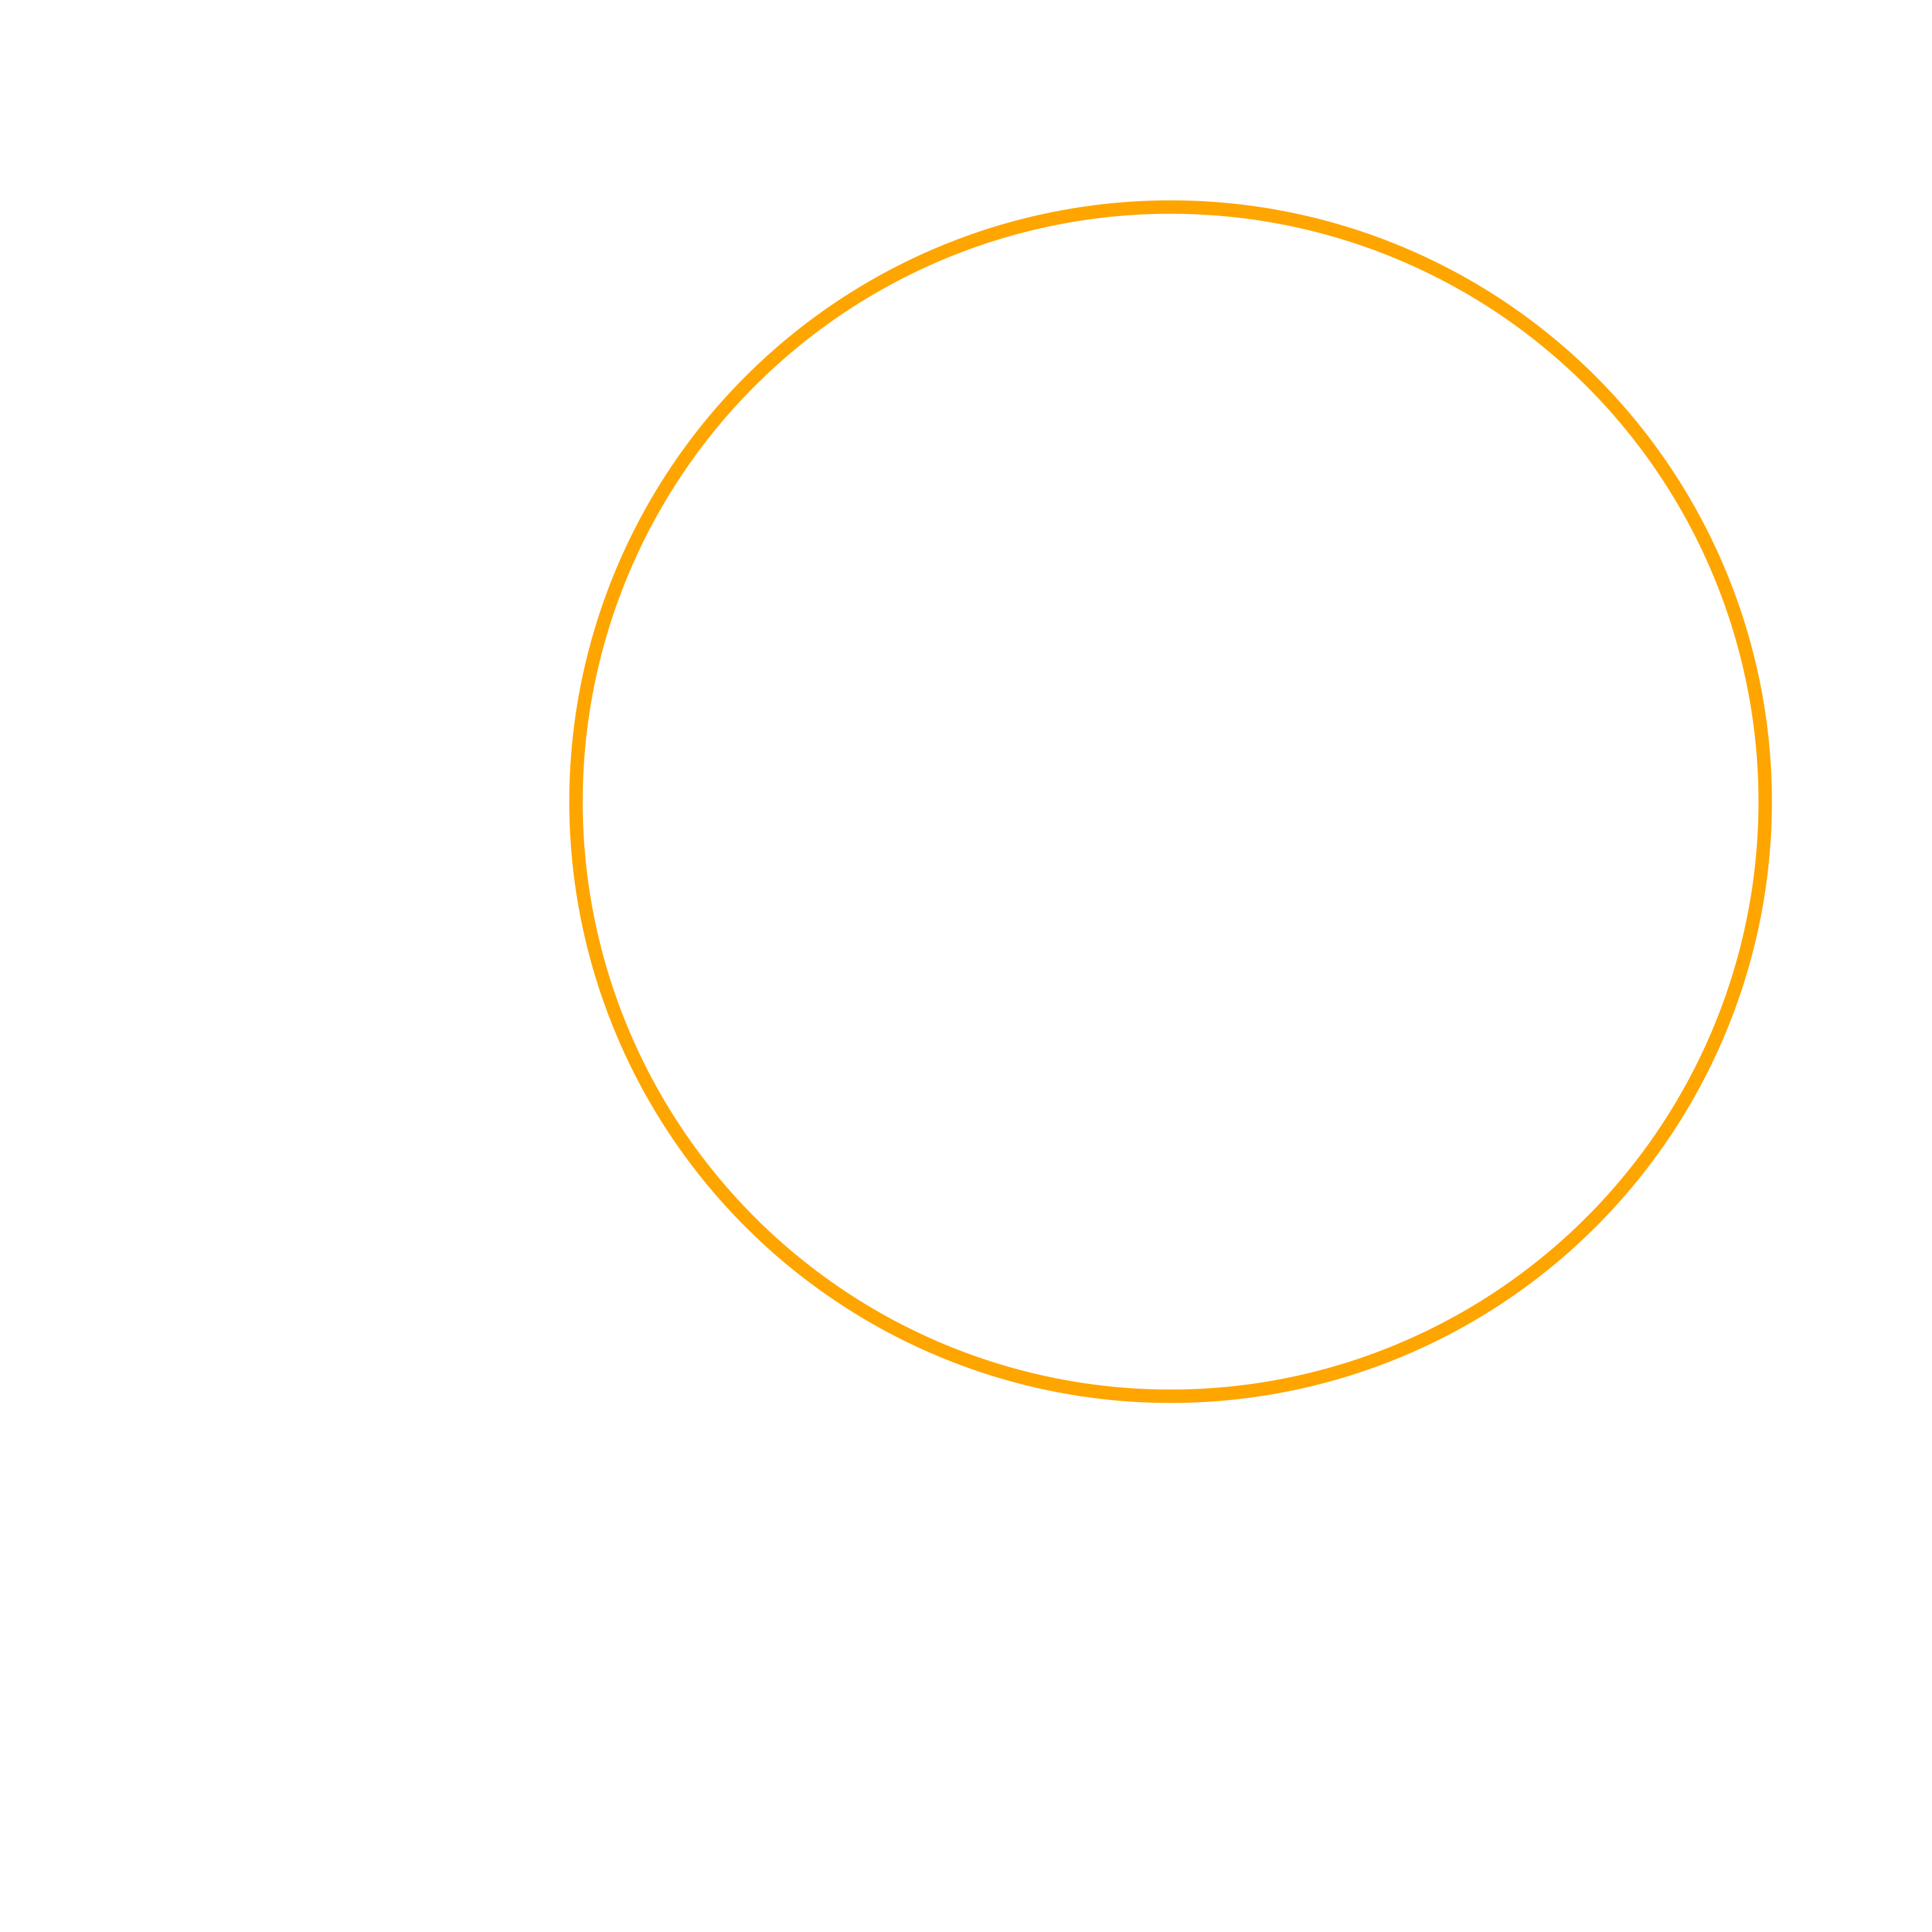
\includegraphics[width=\textwidth]{oscillator_phase_plane}
  \end{minipage}
  \vfill
\end{frame}

\begin{frame}
  \vfill
  \begin{minipage}{.36\textwidth}
    \centering
    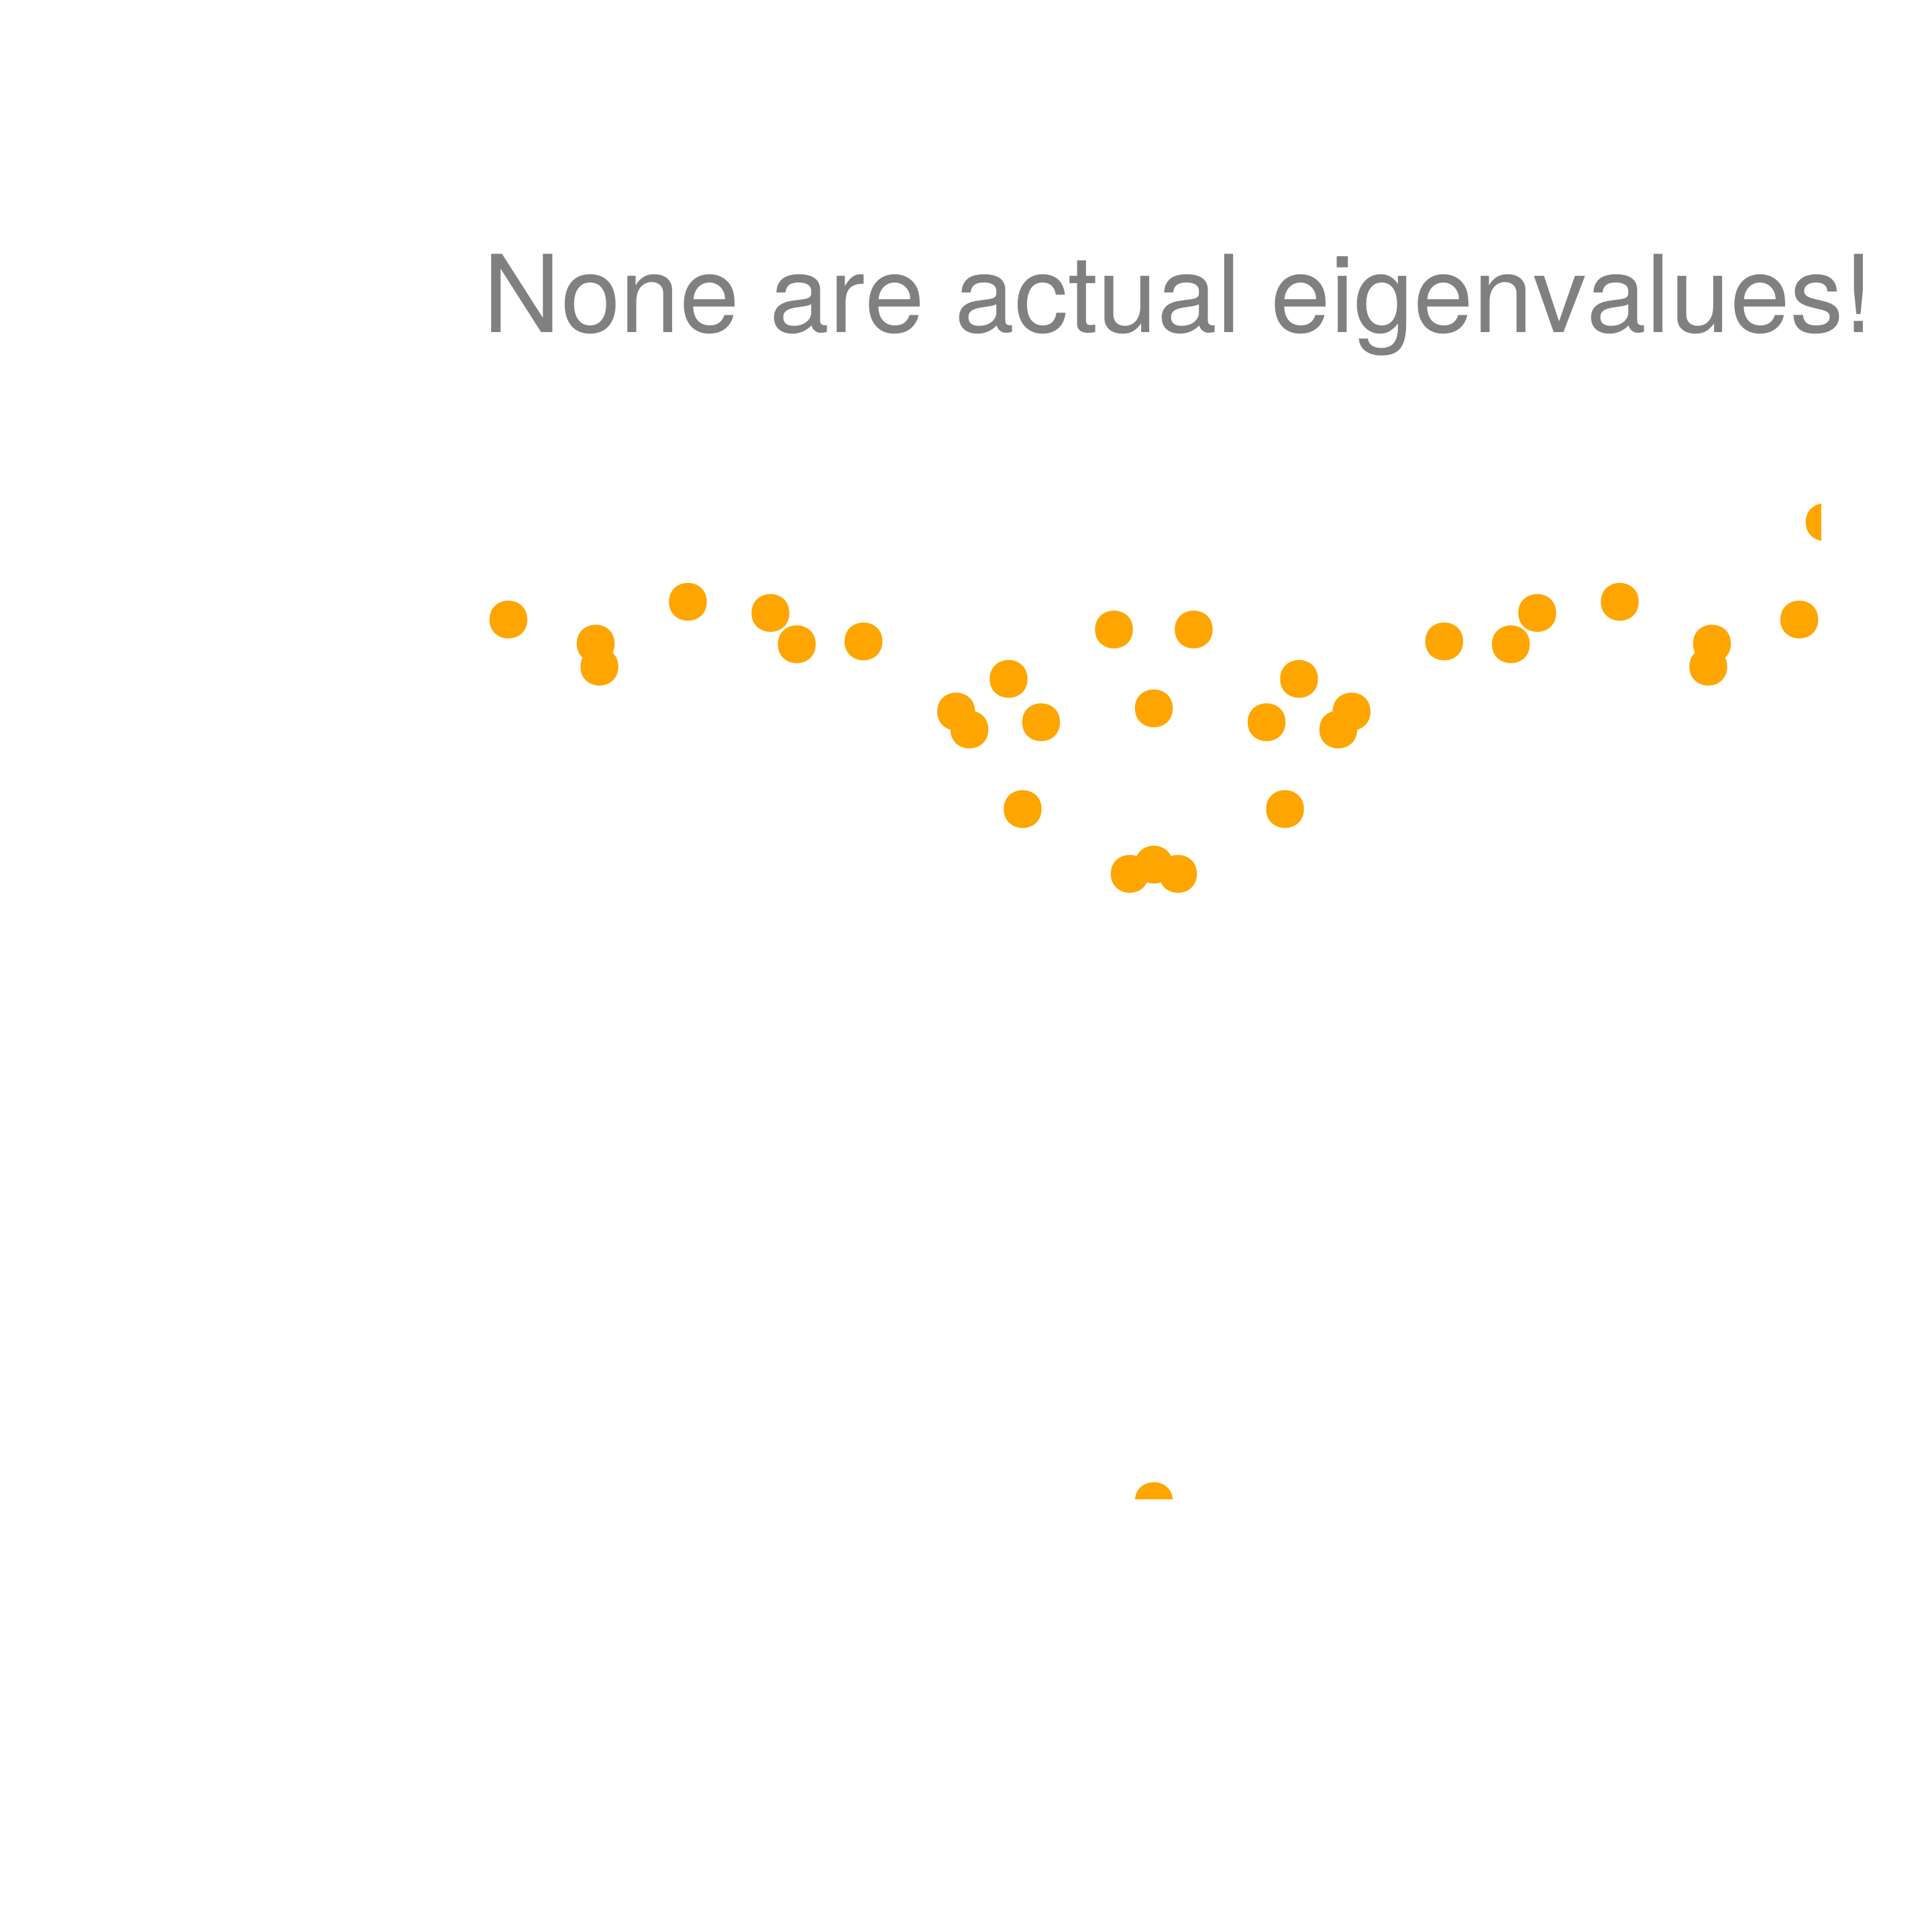
\includegraphics[width=\textwidth]{Lorenz_eigenvalues_residual}
  \end{minipage}%
  \hfill
  \begin{minipage}{.6\textwidth}
    It is not because you can compute eigenvalues of your approximation that they necessarily are eigenvalues of the true Koopman operator !
  \end{minipage}
  \vfill
\end{frame}

\begin{frame}
  \vfill
  \begin{minipage}{.56\textwidth}
    Stay up-to-date with the current literature! A lot has been done since the pioneering work of Peter on DMD.
  \end{minipage}%
  \hfill
  \begin{minipage}{.40\textwidth}
    \centering
    
\includegraphics[width=.9\textwidth]{books}
  \end{minipage}
  \vfill
\end{frame}

{
  \setbeamercolor*{background canvas}{bg=white}
  \setbeamercolor{normal text}{fg=black}
  \usebeamercolor[fg]{normal text}

  \begin{frame}
    \begin{minipage}{.28\textwidth}
      \centering
      
\includegraphics[height=.15\textheight]{github}
    \end{minipage}%
    \hfill
    \begin{minipage}{.68\textwidth}
      \url{https://loiseaujc.github.io/}
    \end{minipage}

    \bigskip

    \begin{minipage}{.28\textwidth}
      \centering
      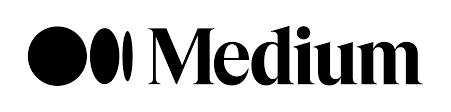
\includegraphics[width=\textwidth]{medium}
    \end{minipage}%
    \hfill
    \begin{minipage}{.68\textwidth}
      \url{https://loiseau-jc.medium.com/}
    \end{minipage}

    \bigskip

    \begin{minipage}{.28\textwidth}
      \centering
      
\includegraphics[height=.15\textheight]{twitter}
    \end{minipage}%
    \hfill
    \begin{minipage}{.68\textwidth}
      \url{@loiseau_jc}
    \end{minipage}

  \end{frame}
}

\begin{frame}
  \vfill
  \flushright

  {
  \Large
  \textbf{Thank you for your attention!}
  }

  \bigskip

  {
  \large
  \textcolor{gray}{
  \textbf{Any question?}
  }
  }
  \vfill
\end{frame}

\end{document}
